\documentclass[twoside,english]{uiofysmaster}

\usepackage{pdfpages}
\usepackage{cite}
\usepackage{epsfig}
\usepackage{caption}
\usepackage{subcaption}
\usepackage[normalem]{ulem}
\usepackage{textcomp}
\usepackage{varioref}

%\bibliography{references}

\author{J\o rgen Eriksson Midtb\o}
\title{How to not minimize a function \\
-- and get away with it.}
\date{June 2015}

\begin{document}
\lstset{language=Python}

\pagenumbering{roman}
\includepdf{front-page.pdf}
\cleardoublepage

\begin{abstract}
This is an abstract text.
\end{abstract}

%\begin{dedication}
%  Til Nina Eriksson
%  \\\vspace{12pt}
%  This is a dedication
%\end{dedication}

% \begin{acknowledgements}
% Takk til Are Raklev for rettleiing, til Lars Dal og Anders Kvellestad for god hjelp, og til Anders Lauvland og Anders Hafreager for gode diskusjonar. Takk til Janne og pappa for alt. Takk også til Bryan Webber, Mona Semb, Tor Gjerrestad, Arild 
% \end{acknowledgements}

\tableofcontents
\listoffigures
\listoftables


\chapter{Supersymmetry}
% \marginpar{Should probably include some math}
% Supersymmetry is a hypothetical extension of the Standard model of particle physics. The present chapter gives a brief introduction to the theory of supersymmetry. The summary is largely based on \cite{Batzing:2013}.

% \section{The Standard Model of Particle Physics}
% The standard model of particle physics has been hugely successful in explaining what our universe consists of and how the constituents interact with each other. But it is well known that the standard model is incomplete, for instance since it gives no explanation for dark matter. There are also more technincal problems with the standard model, such as the hierarchy problem of the Higgs boson mass loop corrections and the arbitrariness of the model parameters.

% The standard model is a quantum field theoretic model and may be stated in terms of a Lagrangian density function $\mathcal{L}$. The features that define the standard model emerge by requiring that it is invariant under the action of certain {\it gauge groups} -- specifically the infamous $U(1)_Y\times SU(2)_L\times SU(3)_C$, where the subscripts stand for {\it hypercharge, left} and {\it colour}, respectively, and refer to the properties that the different fields must have in order to be acted upon by the group transformations. By inserting certain {\it fermionic} field content in the Lagrangian and imposing these symmetries, the model acquires a number of {\it gauge bosons} for the different gauge groups. All these particles are \`{a} priori massless, a requirement to fulfill the gauge symmetry. To give particles their observed mass, then, one adds a scalar field and a corresponding scalar potential of a certain shape. The shape of the potential is such that the $U(1)_Y\times SU(2)_L$ symmetry is {\it spontaneously broken} at a certain energy scale, shifting the degrees of freedom around to give a scalar Higgs boson along with the other gauge bosons, and also giving mass to all particles except the photon. The remaining unbroken symmetries are then the $U(1)_\mathrm{em}$ for electromagnetic and $SU(3)_C$ for strong interactions. 

% The particles that make up the standard model are: the three generations of charged leptons, electron, muon and tau, and their three neutral counterparts, the neutrinos; the three generations of up- and down-type quarks up, down, charm, strange, top and bottom; the electroweak gauge bosons photon, Z and W; the strong gauge bosons, the gluons; and the Higgs boson. 

% \section{Motivations for extending the standard model}
% As mentioned, one of the big problems with the standard model is that is has no candidate for particle dark matter. Observations over the last century have given strong evidence for the existence of some as yet unkown form of matter which is distributed in large quantites all over the universe -- in fact four times as much as our ordinary matter. It is widely believed that this dark matter is some form of particle. Dark matter interacts primarily, or possibly even solely, via gravitation, so the particle has to be colourless and electrically neutral. It also has to be long-lived in order to explain the abundance of it that we still observe. These restrictions rule out most of the standard model particles, with the exception of neutrinos. But neutrinos are known to be very light, almost massless, and calculations of early-universe dynamics show that they are too light to be able to work as dark matter. 

% \section{Extending the standard model by supersymmetry}
% Supersymmetry is a proposed extension of the standard model which increases the number of degrees of freedom by introducing a symmetry between fermions and bosons. The construction of supersymmetry is in a way a two-step process, where one first derives the Lagrangian of a theory with complete symmetry between fermions and bosons, meaning that every bosonic degree of freedom gets a corresponding `supersymmetric' fermionic degree of freedom, and {\it vice versa}. These fields only differ in spin. Then one realizes that this theory cannot be correct, since we have not observed {\it e.g.\ } scalar, colour charged particles with the same mass as the quarks. To make the theory physically viable, the supersymmetric partners must be significantly heavier than their standard model counterparts. 

% \section{The Minimal Supersymmetric Standard Model}




\chapter{Determination of SUSY particle masses from cascade decays}
\label{chap:introducing_the_method}
In the following chapters we will present and discuss a method for determining the masses of supersymmetric particles in certain types of cascade decays. The present chapter formulates the type of process we are studying and the problems we face, and presents a novel method proposed by B. Webber \cite{Webber:2009vm} for making inferrals about the unknown masses. The subsequent chapters deal with confirmation and improvements on the method. We begin by simulating events, adding complexities layer by layer, confirming the method and getting some feeling for its aptitude. We then discuss some problems with the original formulation, suggest ways to amend these and look at ways to develop the method further.

\section{The problem}
Consider the process
\begin{align}
	pp \to \tilde{q}\bar{\tilde{q}} + X, \tilde{q}\bar{\tilde{q}} \to q\bar{q} + 4l + 2\tilde{\chi}_1^0,
\end{align}
proceeding via a two-sided decay chain of the form
\begin{align}
	\tilde{q} \to q + \tilde{\chi}_2^0, \, \tilde{\chi}_2^0 \to l^{\pm} + \tilde{l}^\mp, \, \tilde{l}^\mp \to l^\mp + \tilde{\chi}_1^0\label{eq:goldencascade}
\end{align}
plus the conjugate process. The measurable particles are the two quarks and four leptons, where the lepton pairs are opposite-sign same-flavour. The quantities of interest, however, are the masses of the supersymmetric particles, $m_{\tilde{q}}, m_{\tilde{\chi}_2^0}, m_{\tilde{l}}$ and $m_{\tilde{\chi}_1^0}$. (Potentially with several values for the squarks and sleptons if they differ in generation between the sides.) These are not directly measurable, but the kinematics of the problem depend on them. 

Many methods have been investigated for the purpose of measuring supersymmetric masses. One well known example is the end-point method \cite{1126-6708-2000-09-004}. We measure {\it e.g.}\ the dilepton invariant mass in the process \eqref{eq:goldencascade}. The distribution of the dilepton invariant mass can be shown to form a right triangle where the maximal value is given by
\begin{align}
	(m_{ll}^\mathrm{max})^2 = \frac{ \left( m^2_{\tilde{\chi}_2^0} - m^2_{\tilde{l}} \right) \left( m^2_{\tilde{l}} - m^2_{\tilde{\chi}_1^0} \right)}{m^2_{\tilde{l}}}, \label{eq:invariant_mass_endpoint}
\end{align}
thus constraining $m_{\tilde{\chi}_2^0}$, $m_{\tilde{l}}$ and $m_{\tilde{\chi}_1^0}$. Similar constraints may be obtained for the two other visible particle combinations, giving three equations with three unknowns. This method is very dependent on statistics, since each measured event only contributes one point to the distribution. A large number of events is required to get a reliable value.

\begin{figure}[hbt]
\centering
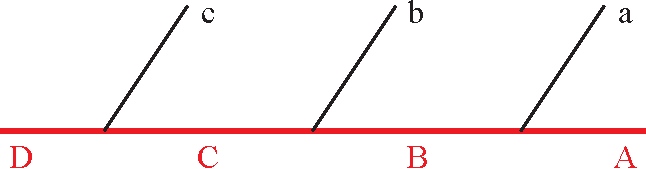
\includegraphics[scale=0.7]{figures/fig-chain.pdf} % Stolen!
\caption{Decay topology.}
\label{fig:decaytree}
\end{figure}

\section{Webber's method}
Webber \cite{Webber:2009vm} suggests a different method, where all kinematical info from every event is used. Consider the general decay tree in figure \ref{fig:decaytree}. Assuming that the decaying particles are on-shell, the 4-momenta in the upper chain should satisfy
\begin{align}
	(p_c + p_b + p_a + p_A)^2 &= M_D^2\nonumber \\
	(p_b + p_a + p_A)^2 &= M_C^2\nonumber \\
	(p_a + p_A)^2 &= M_B^2\label{eq:constraints}\\
	p_A^2 = M_A^2\nonumber
\end{align}
The first three equations give three linear constraints on the invisible 4-momentum $p_A$:
\begin{align}
	-2p_c\cdot p_A &= M_C^2 - M_D^2 + 2p_c\cdot p_b + 2p_c \cdot p_a + m_c^2 \equiv S_1,\nonumber \\
	-2p_b\cdot p_A &= M_B^2 - M_C^2 + 2p_b\cdot p_a + m_b^2 \equiv S_2,\\
	-2p_a\cdot p_A &= M_A^2 - M_B^2 + m_a^2 \equiv S_3. \nonumber
\end{align}
Equivalently the conjugate chain (with primed indices) gets the constraints
\begin{align}
	-2p_{c'}\cdot p_{A'} &= M_{C'}^2 - M_{D'}^2 + 2p_{c'}\cdot p_{b'} + 2p_{c'} \cdot p_{a'} + m_{c'}^2 \equiv S_5,\nonumber \\ 
	-2p_{b'}\cdot p_{A'} &= M_{B'}^2 - M_{C'}^2 + 2p_{b'}\cdot p_{a'} + m_{b'}^2 \equiv S_6,\\
	-2p_{a'}\cdot p_{A'} &= M_{A'}^2 - M_{B'}^2 + m_{a'}^2 \equiv S_7.\nonumber
\end{align}
In addition we have the transverse momentum constraints
\begin{align}
	p_A^x + p_{A'}^x &= p_\mathrm{miss}^x \equiv S_4, \label{eq:Svec_orig} \\
	p_A^y + p_{A'}^y &= p_\mathrm{miss}^y \equiv S_8. \nonumber
\end{align}

The vector $\mathbf{S} = (S_1, S_2, ...)$ thus depends on the eight unknown masses 
\begin{align}
	\mathbf{M} = (M_D^2, M_C^2, M_B^2, M_{A'}^2, M_{D'}^2, M_{C'}^2, M_{B'}^2, M_{A'}^2)
\end{align}
and the visible momenta which are measurable in principle. We define a vector containing the 4-momenta of the invisible final state particles as
\begin{align}
	\mathbf{P} = (p_A^x, p_A^y, p_A^z, E_A, p_{A'}^x, p_{A'}^y, p_{A'}^z, E_{A'}). \label{eq:Pvec}
\end{align}
We then have
\begin{align}
	\mathbf{A}\mathbf{P} = \mathbf{S},\label{eq:APS}
\end{align}
where
\begin{align}
	\mathbf{A} = 2 \begin{pmatrix}
						p_c^x & p_c^y & p_c^z & -E_c & 0 & 0 & 0 & 0 \\
						p_b^x & p_b^y & p_b^z & -E_b & 0 & 0 & 0 & 0 \\
						p_a^x & p_a^y & p_a^z & -E_a & 0 & 0 & 0 & 0 \\
						1/2 & 0 & 0 & 0 & 1/2 & 0 & 0 & 0\\
						0 & 0 & 0 & 0 & p_{c'}^x & p_{c'}^y & p_{c'}^z & -E_{c'} \\
						0 & 0 & 0 & 0 & p_{b'}^x & p_{b'}^y & p_{b'}^z & -E_{b'} \\
						0 & 0 & 0 & 0 & p_{a'}^x & p_{a'}^y & p_{a'}^z & -E_{a'} \\
						0 & 1/2 & 0 & 0 & 0 & 1/2 & 0 & 0
					\end{pmatrix}. \label{eq:Amatrix_orig}
\end{align}
Furthermore, $\mathbf{S}$ may be written as 
\begin{align}
	\mathbf{S} = \mathbf{B} \mathbf{M} + \mathbf{C},\label{eq:SBMC}
\end{align}
where
\begin{align}
	\mathbf{B} = \begin{pmatrix}
					-1 & 1 & 0 & 0 & 0 & 0 & 0 & 0 \\
					0 & -1 & 1 & 0 & 0 & 0 & 0 & 0 \\
					0 & 0 & -1 & 1 & 0 & 0 & 0 & 0 \\
					0 & 0 & 0 & 0 & 0 & 0 & 0 & 0 \\
					0 & 0 & 0 & 0 & -1 & 1 & 0 & 0 \\
					0 & 0 & 0 & 0 & 0 & -1 & 1 & 0 \\
					0 & 0 & 0 & 0 & 0 & 0 & -1 & 1 \\
					0 & 0 & 0 & 0 & 0 & 0 & 0 & 0 \\
	\end{pmatrix}
\end{align}
and
\begin{align}
	\mathbf{C} = ( &2p_c \cdot p_b + 2p_c \cdot p_a + m_c^2, 2 p_2 \cdot p_3 + m_b^2, m_a^2, p_\mathrm{miss}^x, \nonumber \\ 
				   &2p_{c'}\cdot p_{b'} + 2 p_{c'} \cdot p_{a'} + m_{c'}^2, 2 p_{b'} \cdot p_{a'} + m_{b'}^2, m_{a'}^2, p_\mathrm{miss}^y )
\end{align}
With all this, the solution for the invisible 4-momenta given the unknown masses is 
\begin{align}
	\mathbf{P} = \mathbf{A}^{-1} \mathbf{S} = \mathbf{D} \mathbf{M} + \mathbf{E}
\end{align}
where $\mathbf{D} = \mathbf{A}^{-1}\mathbf{B}$ and $\mathbf{E} = \mathbf{A}^{-1}\mathbf{C}$.

The matrix $\mathbf{D}$ and vector $\mathbf{E}$ contain only measurable quantities, hence they only need to be calculated once for every event. For the true value of the unknown masses $\mathbf{M}$, the system should satisfy the on-shell conditions
\begin{align}
	p_{A}^2 &= P_4^2 - P_1 ^2 - P_2^2 - P_3^2 = M_{A}^2, \nonumber\\
	p_{A'}^2 &= P_8^2 - P_5 ^2 - P_6^2 - P_7^2 = M_{A'}^2.
\end{align}
So by calculating $\mathbf{D}_n$ and $\mathbf{E}_n$ for each event $n$, and making a {\it hypothesis} $\mathbf{M}$ for the unknown masses, we can measure the goodness of fit for our hypothesis by the quantity
\begin{align}
	\xi^2(\mathbf{M}) = \sum_n \left[(p_{A}^2)_n - M_A^2\right]^2 + \left[(p_{A'}^2)_n - M_{A'}^2\right]^2. \label{eq:xisquared}
\end{align}
Note that this quantity measures the goodness-of-fit of all the unknown masses equally, since it follows from the constraint equations \eqref{eq:constraints} that {\it e.g.}
\begin{align}
	(p_B^2)_n - M_B^2 &= (p_a + p_A)_n^2 - M_B^2 = \nonumber\\
				  &= (p_a^2)_n + (p_A^2)_n + 2p_a\cdot p_A - M_B^2\nonumber\\
				  &= (p_a^2)_n + (p_A^2)_n - M_A^2 + M_B^2 - m_a^2 - M_B^2\\
				  &= (p_A^2)_n - M_A^2.\nonumber
\end{align}

The point of the method is to minimize $\xi^2$ as a function of $\mathbf{M}$. This is generally an eight-dimensional minimization problem with a very complicated function, and thus not easy to solve. However, in the case of identical chains, it reduces to a much more handleable four-dimensional one. The condition of identical chains can often be satisfied by a combination of vetoing ({\it e.g.} b-jets) and assuming small mass splittings between different generations, thus approximating their masses as equal. 

\section{Making sense of dimensions}\label{sec:dimension_fixing}
The aptness of the method hangs on the invertibility of the matrix $\mathbf{A}$. However, the matrix as it stands in \eqref{eq:Amatrix_orig}, is ill-defined for inversion since not all rows have the same units. The rows 4 and 8, corresponding to the components 4 and 8 of the vector $\mathbf{S}$ \eqref{eq:Svec_orig}, have no dimension, while the other rows have dimension $(\mathrm{mass})^1$. This is reflected in the components of $\mathbf{S}$, which all except 4 and 8 have dimension $(\mathrm{mass})^2$. This means both that the magnitude of the determinant is sensitive to the choice of mass scale (since some rows have non-zero dimension) and that it does not scale properly (since not all rows have the same dimension). This is something that Webber does not comment on, but we take steps to amend both problems.

For the first, we redefine $S_4$ and $S_8$ to be 
\begin{align}
	S_4 &\equiv (p_A^x + p_{A'}^x)^2 = (p_\mathrm{miss}^x)^2, \label{eq:Svec_modified} \\
	S_8 &\equiv (p_A^y + p_{A'}^y)^2 = (p_\mathrm{miss}^y)^2. \nonumber
\end{align}
We do not wish to redefine $\mathbf{P}$ \eqref{eq:Pvec}, so to keep the relationship $\mathbf{S} = \mathbf{A}\mathbf{P}$ we modify rows 4 and 8 of $\mathbf{A}$ to
\begin{align}
	\mathbf{A}_4 &= (p_\mathrm{miss}^x, 0, 0, 0, p_\mathrm{miss}^x, 0, 0, 0),\\
	\mathbf{A}_8 &= (0, p_\mathrm{miss}^y, 0, 0, 0, p_\mathrm{miss}^y, 0, 0),\nonumber
\end{align}
such that $\mathbf{A}$ now is
\begin{align}
	\mathbf{A} = 2 \begin{pmatrix}
						p_c^x & p_c^y & p_c^z & -E_c & 0 & 0 & 0 & 0 \\
						p_b^x & p_b^y & p_b^z & -E_b & 0 & 0 & 0 & 0 \\
						p_a^x & p_a^y & p_a^z & -E_a & 0 & 0 & 0 & 0 \\
						p_\mathrm{miss}^x/2 & 0 & 0 & 0 & p_\mathrm{miss}^x/2 & 0 & 0 & 0\\
						0 & 0 & 0 & 0 & p_{c'}^x & p_{c'}^y & p_{c'}^z & -E_{c'} \\
						0 & 0 & 0 & 0 & p_{b'}^x & p_{b'}^y & p_{b'}^z & -E_{b'} \\
						0 & 0 & 0 & 0 & p_{a'}^x & p_{a'}^y & p_{a'}^z & -E_{a'} \\
						0 & p_\mathrm{miss}^y/2 & 0 & 0 & 0 & p_\mathrm{miss}^y/2 & 0 & 0
					\end{pmatrix}. \label{eq:Amatrix_modified}
\end{align}

This redefinition does not alter the solvability of the problem, since the only information lost in $\mathbf{S}$ is the sign of $p_\mathrm{miss}^i$ which is kept in $\mathbf{A}$ instead. Also it keeps the essential feature that $\mathbf{A}$ only contains measured quantities, such that it can be inverted prior to making a mass hypothesis. The redefinition of $\mathbf{S}$ means we also have to modify $\mathbf{C}$ to keep the relationship $\mathbf{S} = \mathbf{B} \mathbf{M} + \mathbf{C}$ (Eq. \eqref{eq:SBMC}). We thus make the same redefinitions here, {\it i.e.}
\begin{align}
	C_4 &\equiv (p_\mathrm{miss}^x)^2, \label{eq:Cvec_modified} \\
	C_8 &\equiv (p_\mathrm{miss}^y)^2. \nonumber
\end{align}

The other problem was to make the mathematics dimensionless. All elements of $\mathbf{A}$ and $\mathbf{P}$ now have mass dimension 1, while all elements of $\mathbf{S}$, and thus $\mathbf{M}$ and $\mathbf{C}$, have dimension 2. We are free to multiply both sides of Eq. \eqref{eq:APS} by some normalization mass $M_\mathrm{norm}$ squared,
\begin{align}
	\frac{1}{M_\mathrm{norm}^2} \mathbf{A}\mathbf{P} = \frac{1}{M_\mathrm{norm}^2} \mathbf{S},
\end{align}
and we choose to take it into the matrix and vectors such that they all become dimensionless, {\it i.e.}\ we modify
\begin{align}
	\mathbf{\hat A} = \frac{1}{M_\mathrm{norm}}\mathbf{A},\nonumber \\
	\mathbf{\hat P} = \frac{1}{M_\mathrm{norm}}\mathbf{P},\label{eq:vectors_normalized}\\
	\mathbf{\hat S} = \frac{1}{M_\mathrm{norm}^2}\mathbf{S},\nonumber 
\end{align}
thus modifying $\mathbf{M}$ and $\mathbf{C}$ in the same way as $\mathbf{S}$ to comply with Eq. \eqref{eq:SBMC}. We also modify the fitting function $\xi^2$ accordingly, so that it becomes
\begin{align}
	\xi^2(\mathbf{M}) = \sum_n \left[(\hat p_{A}^2)_n - \frac{M_A^2}{M_\mathrm{norm}^2}\right]^2 + \left[(\hat p_{A'}^2)_n - \frac{M_{A'}^2}{M_\mathrm{norm}^2}\right]^2.\label{eq:xisquared_modified}
\end{align}

To obtain numbers of order 1, which is optimal for numerical purposes, we should pick a mass of the relevant scale for the problem. This is not something that is known {\it \`a priori}, since it depends on the supersymmetric masses that we are trying to determine. We might be tempted to use something based on the measured momenta, but this is a bad idea since it would mean weighting different events differently. We choose the normalization constant
\begin{align}
	M_\mathrm{norm} = 100 \,\mathrm{GeV},
\end{align}
the same order of magnitude as we expect for the supersymmetric masses ($\sim$ electroweak scale). 









\section{Taking account of combinatorics}
\label{sec:combinatorics}
In a real detector event, the ordering of the quarks and leptons in and between chains is not known -- all we have are the measured particle's type and momenta. We must take this into account when applying the method. Webber does this by evaluating all possible combinations in each event and selecting the combination which gives the lowest $\xi^2$ value, choosing to add this value to the sum in Eq. \eqref{eq:xisquared_modified}. The number of possible combinations are 8 or 16, depending on whether the lepton pairs in the two chains are the same flavour or not. 

For two pairs of different-generation leptons, the possible orderings are (given some `base ordering' which we permute from): Switching the ordering of the leptons in the upper chain; switching the ordering of the leptons in the lower chain; or switching the leptons in both chains. For each of these permutations we have the option to switch the two quarks, so the total number of combinations is 8. In the case of identical leptons, we may additionally interchange leptons between the chains -- but this only increases the total combinations by a factor of 2 because the same-chain leptons must have opposite charge.

Note that in order to switch the ordering of leptons within the same chain, all we need to do is permute the rows of the matrix $\mathbf{A}$. The vector $\mathbf{C}$ is invariant as long as the same-chain leptons have the same mass. When the quarks are flipped, however, or when leptons are interchanged between chains, then we must redefine $\mathbf{A}$ and $\mathbf{C}$. Webber makes a point that this property can save computer memory, since one only has to store two or four versions of the matrix and vector for each event. This is however not really a big issue with the amount of memory available in modern computers. 












\section{Outline of the plan}
In this thesis we wish to investigate and hopefully develop this method further. We will begin by reproducing Webber's parton level results using Monte Carlo simulations. We will then add layers of realism and complexety approaching something closer to the real experimental situastion, in order to investigate its full potential. In the end we will focus on well motivated scenarios that can be discovered in Run II of the LHC.  Along the way we will also make some improvements on the method.

The plan of attack is as follows:
\begin{enumerate}
	\item We begin by generating squark pairs at rest, decaying them in the chain of on-shell two-body decays given in (\ref{eq:goldencascade}). The visible decay products, quarks and leptons, are then used to reconstruct the masses. As a benchmark we investigate the precision attainable for the parameter point SPS1a~\cite{Allanach:2002nj}. 
	\item Because of final state radiation and parton showering, as well as---to a lesser degree---sparticle widths, the particles in the decay chain will not be on-shell due to extra gluons (and photons) in the final state. We employ a more sophisticated Monte Carlo code, {\tt Herwig++}~\cite{Bahr:2008pv}  to simulate these properties. This should have an effect on the mass reconstruction since Webber's method assumes on-shell decays.
	\item	We then compare results with and without including the combinatorical issues from identifying the decay products, and we add a simple parametrised momentum smearing, based on realistic detector response, in order to simulate that the measurement of the kinematics of final-state particles is not exact. This was the level of precision employed by Webber in~\cite{Webber:2009vm}.
	\item The partons that emerge from the hadron showers will hadronize, forming a hadron jet before arriving in the detector. Measurement of the initial parton from reconstructing such jets is one of the big challenges of collider physics. We use the {\tt FastJet}~\cite{Cacciari:2011ma} program for jet reconstruction, with algorithms used in the LHC experiments, and study the effect of jet reconstruction on the mass measurement.
	\item In an analysis of real data, one would have to use selection criteria such as cuts on transverse momentum and number of jets and leptons to discriminate between signal and background events. We will apply such cut schemes to our simulated events based on expectations for 14 TeV LHC. In addition we simulate the expected largest backgrounds for a four-lepton supersymmetry search and investigate how the performance of the method is affected by the presence of background.
	\item {\bf If time} As a last step towards realism, we put the events through a fast detector simulation. 
	\item We then investigate improvements over the original model. Webber and collaborators \cite{Nojiri:2010dk} propose combining the kinematical best-fit reconstruction with measurements of end points of invariant mass distributions.
	\item Investigating other types of chains. Not-equal-sided? Different number of steps? Fitting a mass plane rather than points?
	\item Finally, we look at a well motivated model taken from \cite{Allanach:2014gsa} that was constructed on the basis of a small excess seen in 8 TeV data by the CMS Collaboration~\cite{CMS:2014jfa}, which would be consistent with the decay chain in (\ref{eq:goldencascade}). We show what precission we can expect from mass measurments at 14 TeV LHC should such a scenario be realized.
\end{enumerate}






























%%%%%%%%%%%%%%%%%%%%%%%%%%%%%%%%%%%%%%%%%%%%%%%%%
\chapter{Investigating Webber's method by Monte Carlo simulations}
\label{ch:MC}
%%%%%%%%%%%%%%%%%%%%%%%%%%%%%%%%%%%%%%%%%%%%%%%%%
Webber demonstrates the aptitude of the method on a Monte Carlo generated dataset. A natural starting point for our study is thus to try to reproduce his results. 

\section{Collider physics}
There are several ways in which a pair of squarks can be produced in $pp$ collisions. The three main categories are: direct pair production of two squarks or a squark-antisquark pair; squark plus gluino with subsequent gluino decay to a squark; and pair production of two gluinos which both subsequently decay to squarks. The mechanism of production affects how much momentum goes into the squark, and thus the momentum of the subsequent decay chain. But our method deals mainly with the internal kinematics of the squark decay, which by Lorentz invariance is independent of squark momentum. The only variables in our analysis which explicitly depends on the overall event kinematics is the missing transverse momentum. The three different categories also determine how many hard colour jets are present in the event, which affects the combinatorical aspects of reconstructing the chain. This will be discussed in detail later.\marginpar{Better remember to discuss it in detail.}

\section{Reproducing Webber's results}
Webber uses Fortran {\scshape HERWIG} version 6.510 \cite{Corcella:2000bw,Moretti:2002eu} to produce events, selecting only events where both the squarks are left-handed first- or second generation (to limit the mass splitting), but irrespective of the hard production process. He does his analysis, {\it i.e.} minimization of the $\xi^2$, on 100 samples of 25 events each, using the Minuit Simplex \cite{James:1975dr} routine for minimization. He models the effects of measurement errors in a real detector by applying momentum smearing according to a gaussian distribution, and he puts a cut on the total $\xi^2$ obtained at the minimum to eliminate samples which give a bad result. His results are summarized in table 1 of \cite{Webber:2009vm}, which we for convenience show in table \vref{table:webber_original}. The column $\delta p/p$ indicates the standard deviation of the gaussian smearing applied on the momenta, $\xi^2_\mathrm{max}$ indicates the cut value of the $\xi^2$, $f_\xi$ is the fraction of samples surviving the cut and $f_\mathrm{cor}$ is the fraction of events where the chosen particle combination (selected as described in section \ref{sec:combinatorics}) is the correct one. 


\begin{table}[hbt]
	\centering
	\begin{tabular}{| l | l | l | l  || l | l | l | l |}
		\hline
		$\delta p/p$ & $\xi^2_\mathrm{max}$ & $f_\xi$ & $f_\mathrm{cor}$ & $m_{\tilde q} (540)$ & $m_{\tilde \chi_2^0} (177)$ & $m_{\tilde l} (143)$ & $m_{\tilde \chi_1^0} (96)$ \\
		\hline \hline
		0 & 	$\infty$ &	100 \%	& 72 \%	& $538 \pm 20$	&	$176 \pm 12$	&	$143 \pm 7$	& 	$95 \pm 10$	\\
		0 &		100 &		80 \%	& 76 \% & $539 \pm 7$	&	$177 \pm 1$		&	$144 \pm 1$	&	$96 \pm 2$	\\
		5 \% &	$\infty$ &	100 \%	& 52 \% & $534 \pm 28$	& 	$176 \pm 11$	&	$143 \pm 10$&	$95 \pm 13$ \\
		5 \% &	100 &		57 \%	& 55 \% & $539 \pm 9$	&	$178 \pm 3$		& 	$144 \pm 2$	&	$96 \pm 4$	\\
		10 \% &	$\infty$ &	100 \%	& 40 \% & $522 \pm 37$	&	$171 \pm 18$	&	$140 \pm 17$&	$88 \pm 26$	\\
		10 \% &	200 &		42 \%	& 43 \% & $530 \pm 22$	& 	$173 \pm 12$	&	$140 \pm 12$&	$89 \pm 20$ \\
		\hline
	\end{tabular}
	\caption{Webber's table of results, taken from p. 6 of \cite{Webber:2009vm}.}
	\label{table:webber_original}
\end{table}

\begin{figure}[hbt]
	\centering
	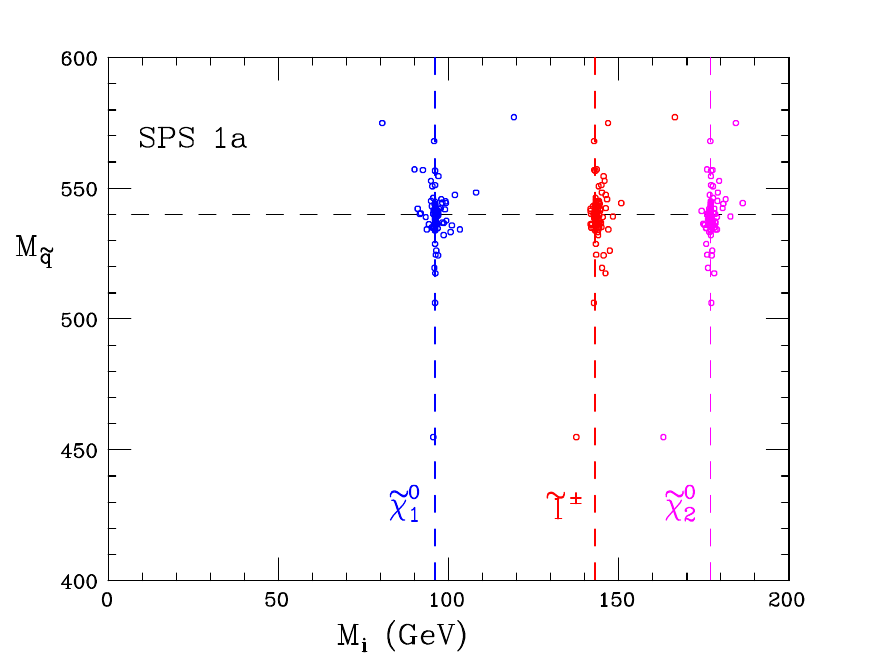
\includegraphics[width=0.8\textwidth]{figures/webber_rec_table/webber_scatter.png} 
	\caption{Figure 2 from \cite{Webber:2009vm}, displayed here for convenience.}
	\label{fig:webber_scatter}
\end{figure}

We have made a thorough investigation of these results using a variety of tools. We have generated Monte Carlo events using both Herwig++ 2.7.1  \cite{Bahr:2008pv} and Pythia 8.2 \cite{Sjostrand:2014zea}. We have implemented the Simplex algorithm in various versions as well as other minimization algorithms for the fit. Webber himself also very generously sent us his own MC generation code, so we were able to make a quite close reconstruction of his analysis. But in the process of confirming his results, we have discovered what appears to be an error in the analysis. The error has to do with the choice of tolerance in the minimization routine. To understand this, we have to briefly discuss the Simplex algorithm.

\subsubsection{The Nelder-Mead Simplex algorithm}

{\scshape Simplex} \cite{nelder1965simplex} is a heuristic minimization search method for minimizing a scalar function of $N$ variables. It takes a starting parameter point as input from the user. From this parameter point it erects a {\it simplex}, an ``$N+1$-dimensional triangle''. It then begins to evaluate the function in the vertices of this simplex. A new simplex is constructed by reflecting the vertex with the highest function value around the (hyper)line made out of the other $N$ vertices. Hopefully this new simplex lies lower in the function terrain, and thus the algorithm iterates towards a local minimum. In case of trouble, it may also try contracting the simplex or distorting its shape in various ways to obtain points of lower function values. Since the method is heuristic, so is the convergence criterion. Convergence is said to be obtained when the {\it estimated distance to minimum (EDM)} is smaller than some set tolerance value. Usually there is also a predefined maximal number of iterations before the method gives up, to avoid going on forever on non-converging problems. The EDM is defined as

\begin{align}
	\mathrm{EDM}(f_\mathrm{min},f_\mathrm{max}) = \frac{|f_\mathrm{max}-f_\mathrm{min}|}{|f_\mathrm{max}| + |f_\mathrm{min}|},
\end{align}
where $f_\mathrm{min}$ and $f_\mathrm{max}$ are the function values at the lowest and highest point of the current simplex, respectively. This means that the convergence criterion really measures how ``flat'' the function is. If the tolerance is too high, then, we run the risk of obtaining convergence in a region far from the minimum, but where the gradient is not steep enough to be resolved by the set tolerance.

A pitfall of any minimization routine, also for Minuit Simplex, is that it has a default tolerance value which is used automatically unless the user specifically changes it. Minuit is often used for minimizing $\chi^2$ and log-likelihood functions, where the scale of the function is predetermined. For our problem, however, there is no such absolute scale. We have chosen to normalize the $\xi^2$ in units of $100 \, \mathrm{MeV}$, but this is just an ad-hoc choice that we observe gives numbers of order one in our calculations. There is no probabilistic interpretation of $\xi^2$, as Webber himself notes (footnote 1, p. 4 of \cite{Webber:2009vm}). The normalization 

The default tolerance in Minuit Simplex is 0.1. This appears to be what Webber has used, since we obtain much the same results when choosing a similar value. But this does not resolve the function well enough, and leads to convergence at a non-minimal point. If additionally, as is the case here, the search is started at or close to the best-fit point we believe in (in our case, the masses used to generate the Monte Carlo), then the minimization may obtain ``convergence'' at points very close to the optimal, but these points are not minimal points, just quite flat. If our goal is to get the minimal to be close to the true value, then we might be easily fooled.

% This appears to be what has happened in Webber's analysis. Refer to the scatter plot in figure 2 of \cite{Webber:2009vm}, displayed in figure \ref{fig:webber_scatter} for convenience. When we try to reproduce the results, we discover that we get very similar behaviour with a tolerance of order 0.1, while decreasing the tolerance dramatically alters the results. This is illustrated in the scatter plots shown in figure \ref{fig:webber_rec_scatter_tolerance-comparison}, where the same Herwig++ dataset is minimized with high and low tolerance, respectively.\footnote{Note that the SUSY masses used for the Monte Carlo, here and in the following, differ slightly from those Webber uses -- this is due to differences between RGE running programs.} We see that the former case compares well to Webber's scatter plot, and also the mean value and errors on the masses agree quite well. When the tolerance is decreased, however, the minimization search spreads out, and there is a bias toward lower mass values. These tendencies can be understood physically, as we will come back to. \marginpar{Remember to discuss the degenerate direction, valley behaviour and LSP resolution at some point}

\subsubsection{The tolerance is too high}

This appears to be what has happened in Webber's analysis. Refer to the scatter plot in figure 2 of \cite{Webber:2009vm}, displayed in figure \vref{fig:webber_scatter} for convenience. This scatter plot shows the fit corresponding to the first row of table \ref{table:webber_original}. We have reproduced this fit using Webber's own code -- albeit with one modification: Since we don't have access to the old ISAJET and ISAWIG software for RGE running of SUSY parameters, we have generated our SPS 1a parameter point using {\scshape SoftSUSY} version 3.4.1 \cite{Allanach:2001kg}, and converted the resulting SLHA \cite{Skands:2003cj} model file to ISAWIG format using the package {\scshape PySLHA} version 3.0.2\footnote{We actually had to do some work on the {\scshape PySLHA} code to fix quite a few errors in the formatting of the ISAWIG file. We have sent our edits to the {\scshape PySLHA} author, and they will be included in a future version.} \cite{Buckley:2013jua}. The effects of using a different RGE runner is that the SUSY masses are not exactly equal. The most significant shift is the squarks, which in Webber's case have a mass of 540 GeV, compared to 565 GeV in our case. We find that we get much the same type of results as Webber gives in his article.\marginpar{Should we reproduce Webber's original table for our ISAWIG file, i.e. minimize with default settings, just to have strict scrutiny?} Our reproduction of figure \ref{fig:webber_scatter} is shown in figure \vref{fig:webber_rec_scatter_tolerance-comparison} (subfigure a). 

\begin{figure}[hbt]
	\centering
	\begin{subfigure}[b]{0.6\textwidth}
		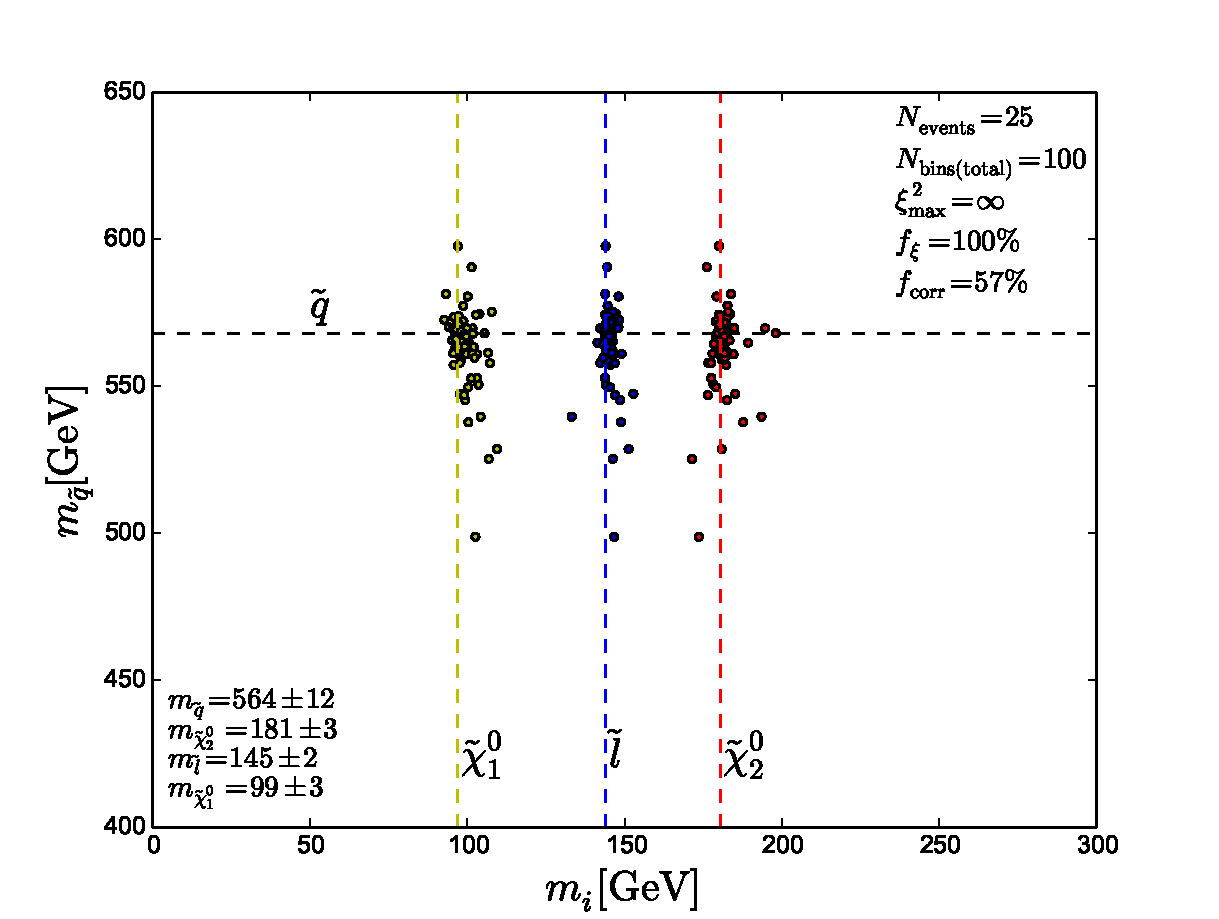
\includegraphics[width=\textwidth]{figures/webber_rec_table/webber_HW-rec_hightol_nocut.pdf} 
		\caption{ }
	\end{subfigure}

	\begin{subfigure}[b]{0.6\textwidth}
		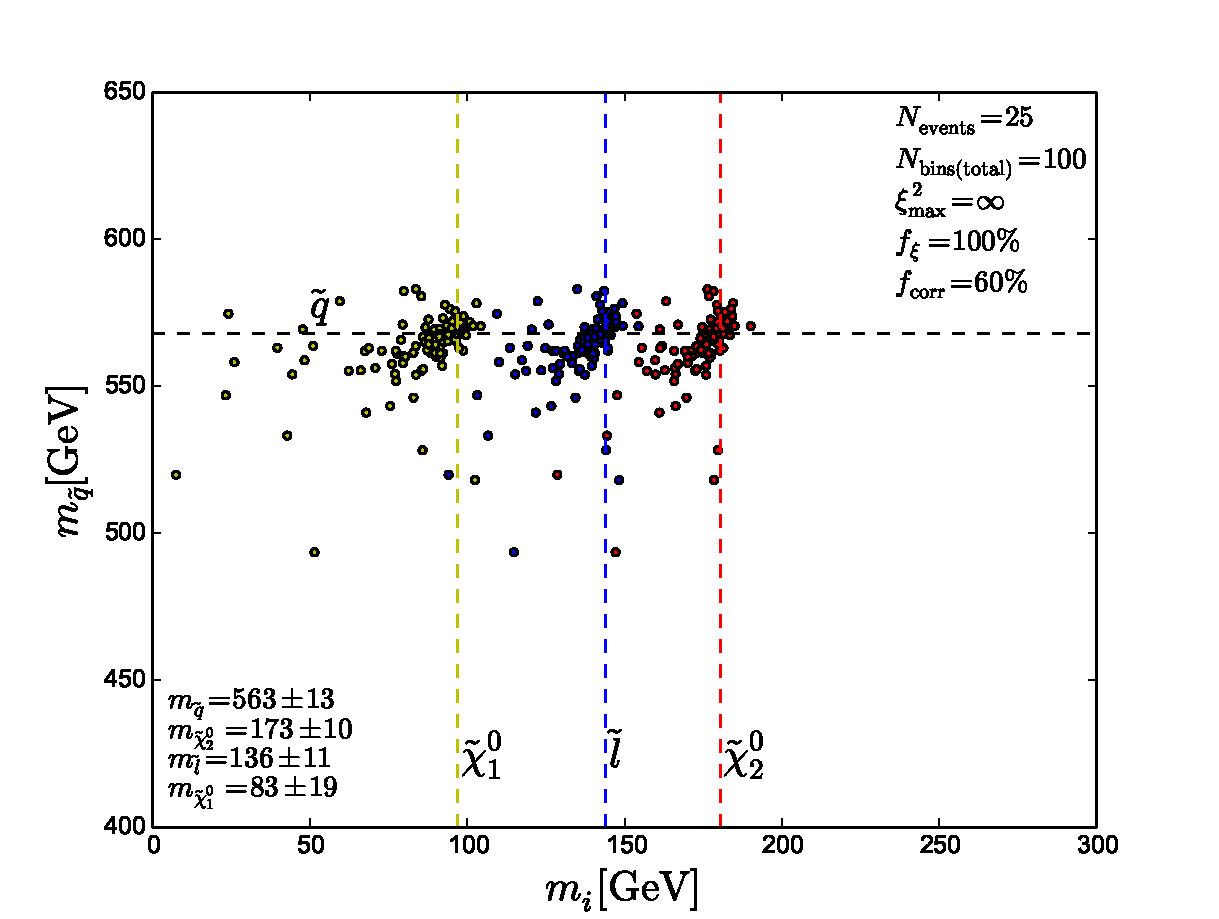
\includegraphics[width=\textwidth]{figures/webber_rec_table/webber_HW-rec_nocut.pdf}
		\caption{ } 
	\end{subfigure}
	\caption{Reproduction of Webber's fit (corresponding to figure \ref{fig:webber_scatter} and the first row of table \ref{table:webber_original}) for (a) original convergence tolerance and (b) a lower tolerance criterion.}
	\label{fig:webber_rec_scatter_tolerance-comparison}
\end{figure}

However, the tolerance setting in {\scshape Minuit} can be adjusted. When we rerun the code used to produce figure \ref{fig:webber_rec_scatter_tolerance-comparison} (a) with the tolerance set to $10^{-12}$, we get the fit shown in \ref{fig:webber_rec_scatter_tolerance-comparison} (b). The results are not dramatically altered, but there are some features to notice: There is a clear tendency that the points lie along a line making about $45^\circ$ with the vertical, going southwest-northeast. This is a feature we should expect physically: If the fit reduces one of the masses, {\it e.g.\ } the squark, then this should affect the fit of the other masses, reducing them correspondingly.\footnote{This is part of the reason why these kinds of mass reconstruction methods very often reconstruct the squared mass {\it difference} rather than the masses themselves.} We also note that the masses are almost always lower than the true value, {\it i.e.\ } there is a bias in the fit. The fact that this physically reasonable degenerate direction appears when the tolerance is reduced indicates that a such a reduction is necessary to acheive correct results. Finally we note that while the mean value and errors on the masses are not that much worse than in the original fit, their accuracy is somewhat reduced. Particularly so for the LSP, where the fit is reduced from $99 \pm 3$ GeV to $83 \pm 19$ GeV (true value 97 GeV).

These fit results, with the low tolerance setting, are still not bad. However, in table \ref{table:webber_original}, Webber also gives best-fit values where he has applied smearing to the 4-momenta, as a crude approximation to the effects of limited detector resolution, {\it etc}. In figure \ref{fig:webber_rec_scatter_tolerance-comparison_10pmomsmear} we show scatter plots of the fits to the dataset smeared with $\delta p/p = 10 \%$, minimized with original and reduced tolerance, again using Webber's own code for event generation and minimization. The fit with original tolerance is consistent with figure 3 of \cite{Webber:2009vm}, as it should be. However, when the tolerance is reduced, the fit results are worsened considerably. Since each event is smeared individually, this appears to greatly affect the position of the minimum. Again we see that the LSP (yellow) recieves the roughest treatment, being pushed to much lower values than the true one in most cases.

\begin{figure}[hbt]
	\centering
	\begin{subfigure}[b]{0.6\textwidth}
		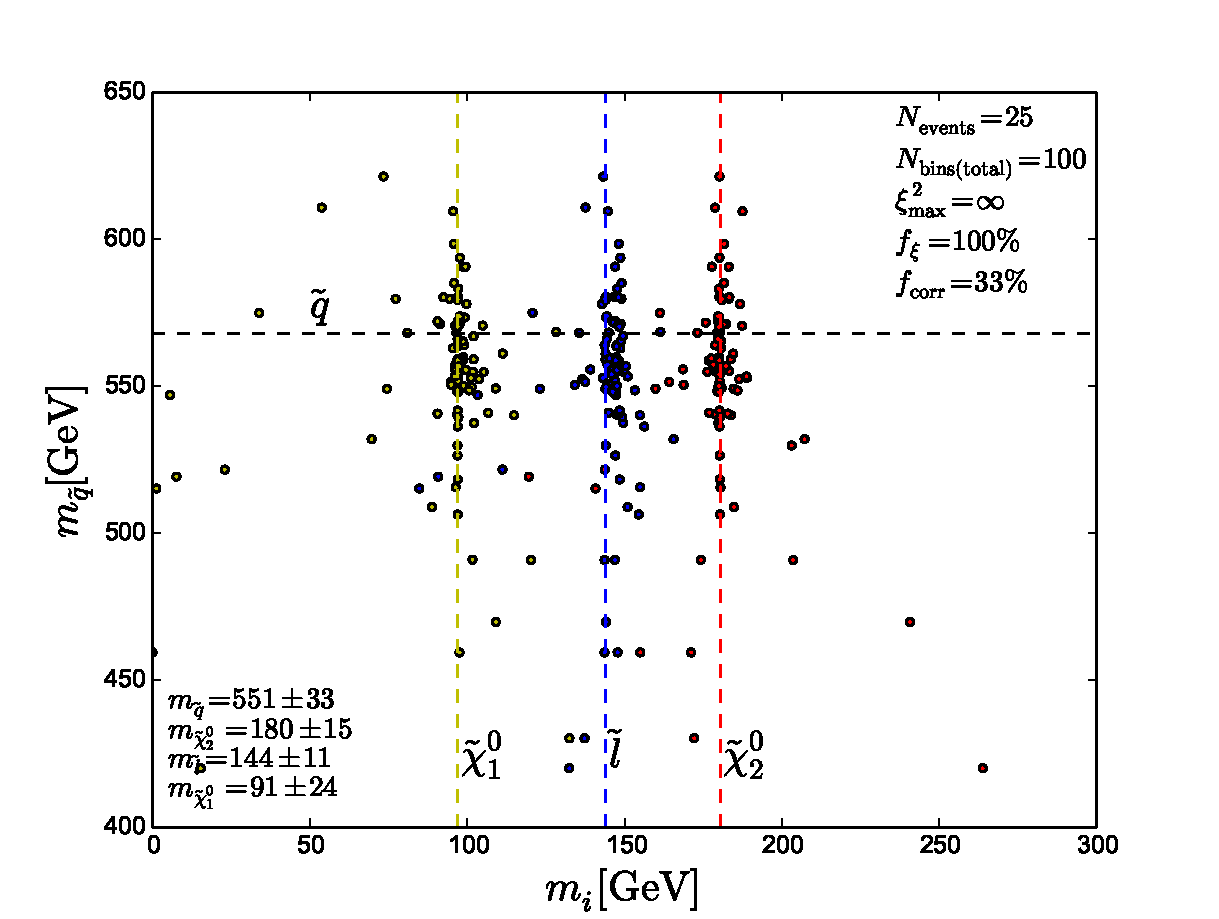
\includegraphics[width=\textwidth]{figures/webber_rec_table/webber_HW-rec_OFL_minuit-minimizer_hightol_10pmomsmear_nocut.pdf} 
		\caption{ }
	\end{subfigure}

	\begin{subfigure}[b]{0.6\textwidth}
		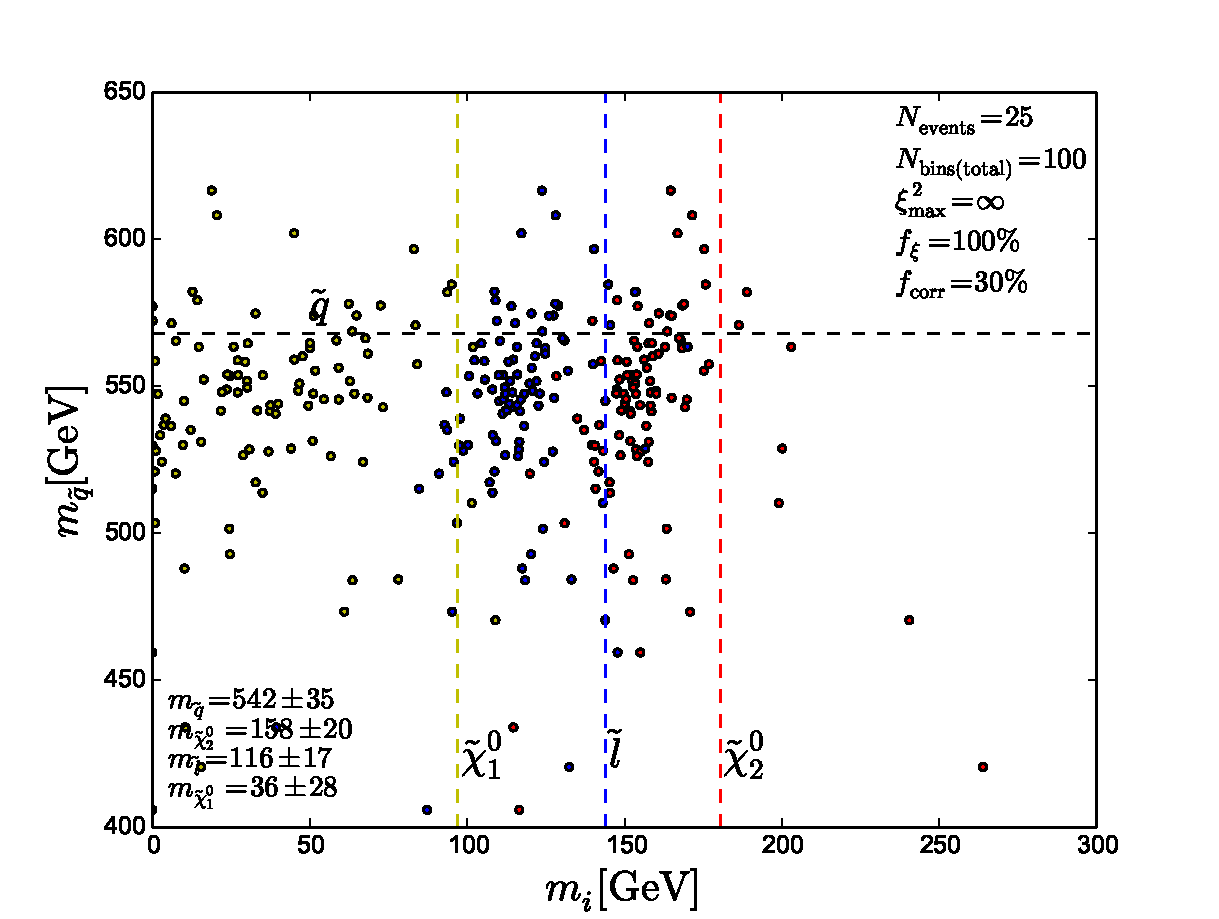
\includegraphics[width=\textwidth]{figures/webber_rec_table/webber_HW-rec_OFL_minuit-minimizer_lowtol_10pmomsmear_nocut.pdf}
		\caption{ } 
	\end{subfigure}
	\caption{Reproduction of Webber's momentum-smeared fit (corresponding to figure 3 of \cite{Webber:2009vm} and the fifth row of table \ref{table:webber_original}) for (a) original convergence tolerance and (b) a lower tolerance criterion.}
	\label{fig:webber_rec_scatter_tolerance-comparison_10pmomsmear}
\end{figure}

However, Webber also investigates the effects of imposing a {\it cut} on the $\xi^2$ value obtained at the minimum. In his fits, this cut tends to remove the bad events, giving a better fit. Applying a cut also helps for the reduced-tolerance fit, although it doesn't salvage everything. In table \ref{table:webber_rec_lowtol} we reproduce table \ref{table:webber_original} for the reduced-tolerance fit. We note that the fraction of samples passing the $\xi^2$ cut is drastically reduced compared to table \ref{table:webber_original}. The fraction of events where the best-fit combination is the true one is also reduced by about half. 


\begin{table}[hbt]
	\centering
	\begin{tabular}{| l | l | l | l  || l | l | l | l |}
		\hline
		$\delta p/p$ & $\xi^2_\mathrm{max}$ & $f_\xi$ & $f_\mathrm{cor}$ & $m_{\tilde q} (568)$ & $m_{\tilde \chi_2^0} (180)$ & $m_{\tilde l} (144)$ & $m_{\tilde \chi_1^0} (97)$ \\
		\hline \hline
		0 & 	$\infty$ &	100 \%	& 36 \%	& $563 \pm 13$	&	$173 \pm 10$	&	$136 \pm 11$	& 	$83 \pm 19$	\\
		0 &		100 &		35 \%	& 52 \% & $565 \pm 9$	&	$175 \pm 8$		&	$138 \pm 9$	&	$86 \pm 16$	\\
		5 \% &	$\infty$ &	100 \%	& 31 \% & $557 \pm 27$	& 	$165 \pm 17$	&	$125 \pm 15$&	$58 \pm 27$ \\
		5 \% &	100 &		13 \%	& 43 \% & $558 \pm 14$	&	$164 \pm 11$	& 	$126 \pm 12$	&	$65 \pm 22$	\\
		10 \% &	$\infty$ &	100 \%	& 29 \% & $542 \pm 35$	&	$158 \pm 20$	&	$116 \pm 17$&	$36 \pm 28$	\\
		10 \% &	200 &		15 \%	& 33 \% & $549 \pm 20$	& 	$155 \pm 12$	&	$116 \pm 12$&	$38 \pm 25$ \\
		\hline
	\end{tabular}
	\caption{Reproduction of the fits in table \ref{table:webber_original} but with reduced convergence tolerance.}
	\label{table:webber_rec_lowtol}
\end{table}

% \begin{figure}[hbt]
% 	\centering
% 	\begin{subfigure}[b]{0.6\textwidth}
% 		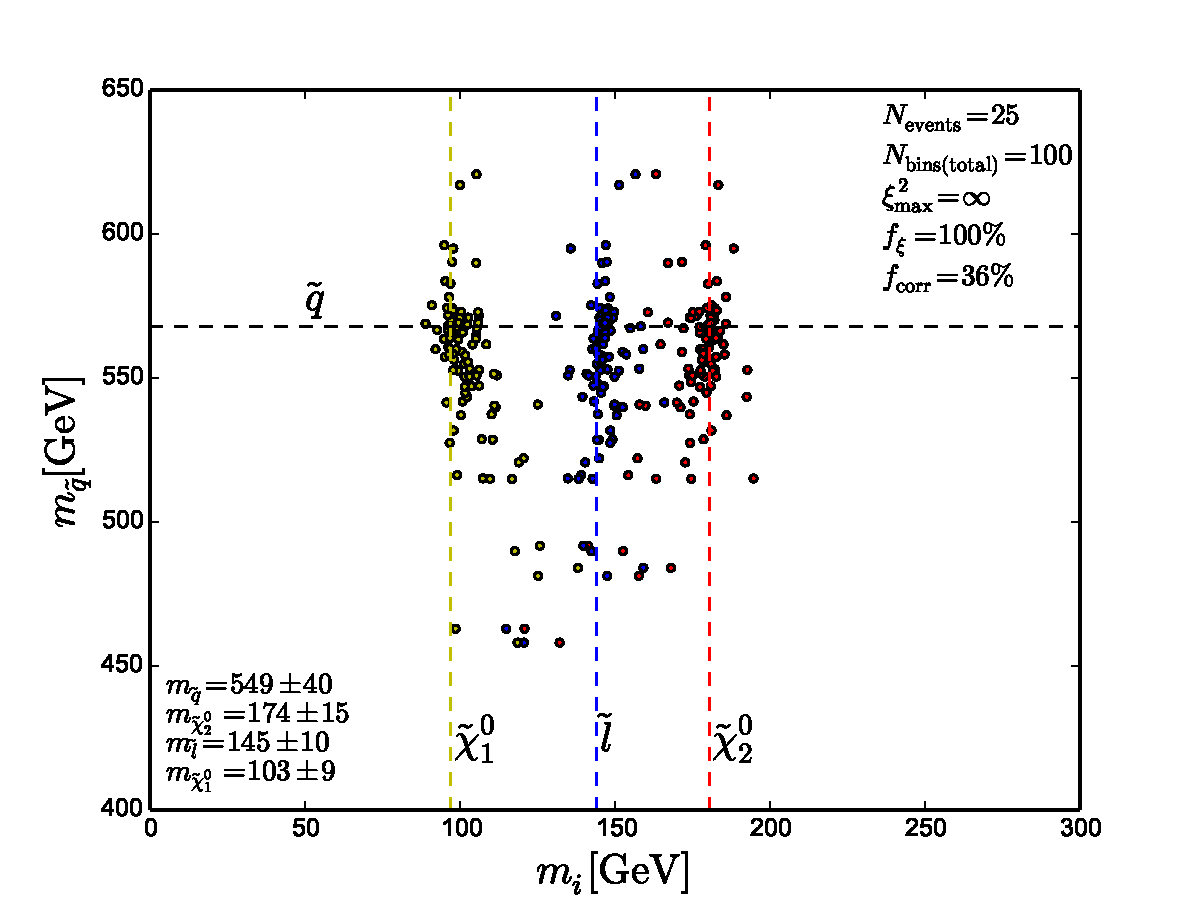
\includegraphics[width=\textwidth]{figures/webber_rec_table/high-tol.pdf} 
% 		\caption{ }
% 	\end{subfigure}

% 	\begin{subfigure}[b]{0.6\textwidth}
% 		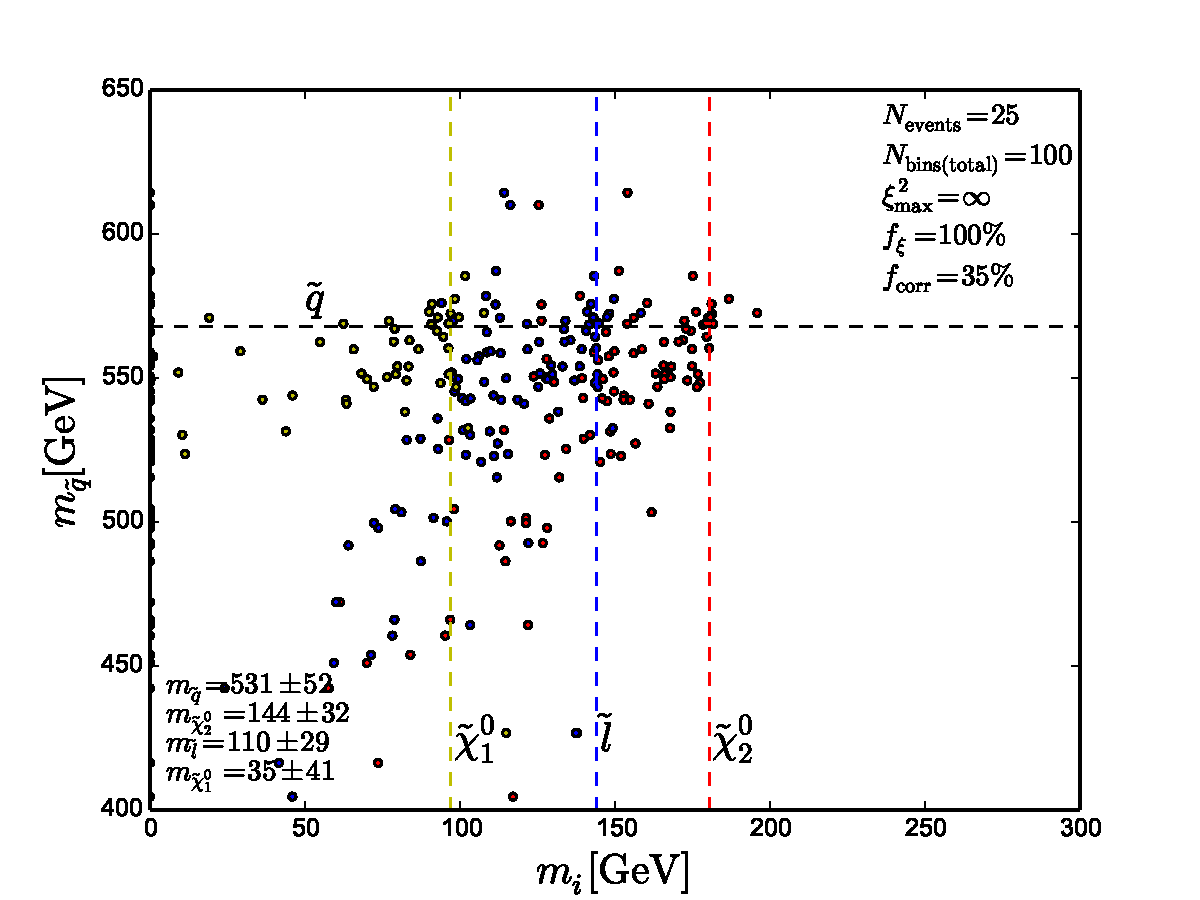
\includegraphics[width=\textwidth]{figures/webber_rec_table/low-tol.pdf}
% 		\caption{ } 
% 	\end{subfigure}
% 	\caption{Minimization on the same dataset for high tolerance (a) and lower tolerance (b).}
% 	\label{fig:webber_rec_scatter_tolerance-comparison}
% \end{figure}

% In the process of understanding Webber's results we have compiled a similar table to \ref{table:webber_original}, table \ref{table:webber_rec}. We have played with the tolerance until we obtained something which resembles Webber's results, mainly focusing on the mean value and standard error on the best-fit masses. We note that we consistently get a significantly lower fraction of events accepted by $\xi^2$ cuts, and also significantly less events where the best-fit point has the correct combinatorical choice. The reasons for these discrepancies are not apparent -- generally it is very difficult to reproduce these kinds of results without knowing the details of the settings in the Monte Carlo event generation and minimization.

% \begin{table}[hbt]
% 	\centering
% 	\begin{tabular}{| l | l | l | l  || l | l | l | l |}
% 		\hline
% 		$\delta p/p$ & $\xi^2_\mathrm{max}$ & $f_\xi$ & $f_\mathrm{cor}$ & $m_{\tilde q} (568)$ & $m_{\tilde \chi_2^0} (180)$ & $m_{\tilde l} (144)$ & $m_{\tilde \chi_1^0} (97)$ \\
% 		\hline \hline
% 		0 & 	$\infty$ &	100 \%	& 36 \%	& $549 \pm 40$	&	$174 \pm 15$	&	$145\pm 10$	& 	$103 \pm 9$	\\
% 		0 &		100 &		35 \%	& 52 \% & $562 \pm 9$	&	$180 \pm 2$		&	$146 \pm 2$	&	$98 \pm 4$	\\
% 		5 \% &	$\infty$ &	100 \%	& 31 \% & $549 \pm 53$	& 	$174 \pm 15$	&	$146 \pm 7$&	$103 \pm 10$ \\
% 		5 \% &	100 &		13 \%	& 43 \% & $563 \pm 9$	&	$180 \pm 2$		& 	$147 \pm 2$	&	$99 \pm 4$	\\
% 		10 \% &	$\infty$ &	100 \%	& 29 \% & $540 \pm 57$	&	$177 \pm 14$	&	$150 \pm 9$&	$104 \pm 13$	\\
% 		10 \% &	200 &		15 \%	& 33 \% & $565 \pm 14$	& 	$182 \pm 3$		&	$149 \pm 2$&	$97 \pm 6$ \\
% 		\hline
% 	\end{tabular}
% 	\caption{Attempt at achieving similar fit results as in \cite{Webber:2009vm}.}
% 	\label{table:webber_rec}
% \end{table}

\subsubsection{The starting-point dependence of the best-fit point}

But what is really the problem with Webber's analysis? After all, he gets great results: He shows that the method very often yields best-fit values close to the true values, which is what we want. The problem is that he (and we) know where to expect the best-fit point to be, since it is input into the Monte Carlo by us. And this is where we start the best-fit search. In a real experiment, these parameters are exactly the unknowns we wish to find. So we must investigate what happens if we start our search in some other point. We have done this, and discover that this greatly affects the location of the best-fit points. In figure \ref{fig:starting_point_sensitivity_combinatorics} we show the best-fit points for four low-tolerance minimizations on the {\scshape HERWIG} dataset. Subfigure (a) is the same as \ref{fig:webber_rec_scatter_tolerance-comparison} (b), the minimization started from the true mass point (TMP). The other three are minimizations from other starting points, selected more or less at random. It is obvious that the fit is hugely dependent on where we start the search.

\begin{figure}[hbt]
	\centering
	\begin{subfigure}[b]{0.45\textwidth}
		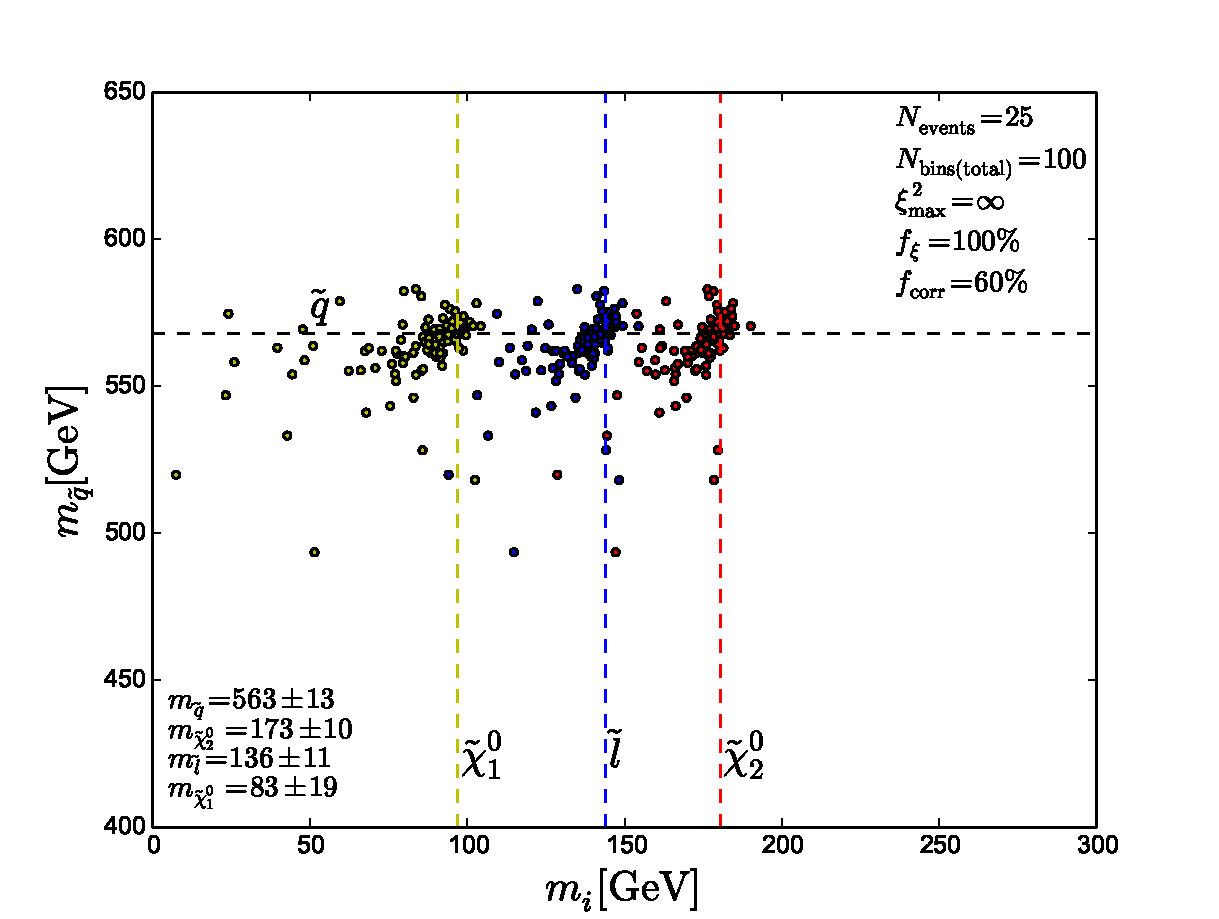
\includegraphics[width=\textwidth]{figures/webber_rec_table/webber_HW-rec_nocut.pdf} 
		\caption{ }
	\end{subfigure}
	\begin{subfigure}[b]{0.45\textwidth}
		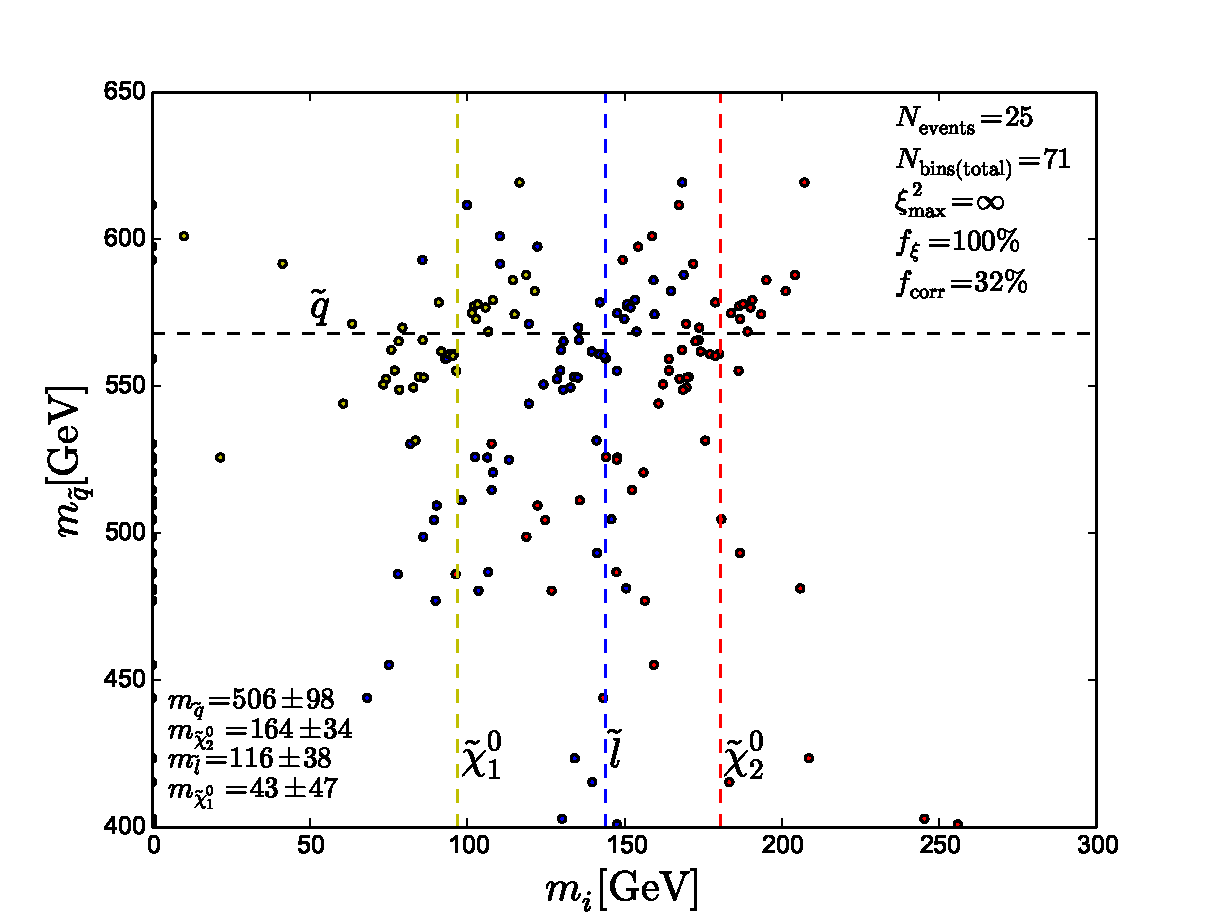
\includegraphics[width=\textwidth]{figures/webber_rec_table/webber-rec_wrong_starting_point-400-300-200-100_lowtol.pdf}
		\caption{ } 
	\end{subfigure}

	\begin{subfigure}[b]{0.45\textwidth}
		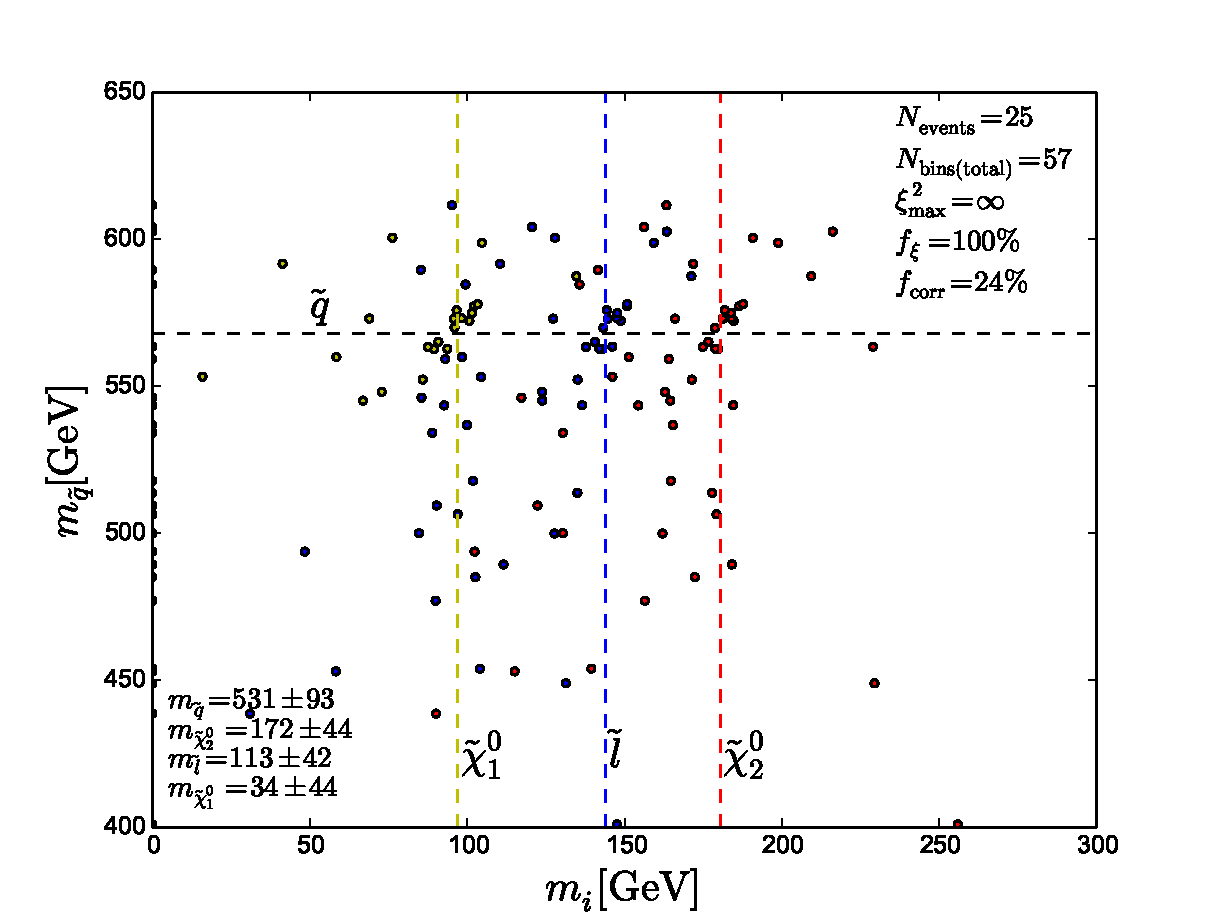
\includegraphics[width=\textwidth]{figures/webber_rec_table/webber-rec_wrong_starting_point-800-500-300-50_lowtol.pdf} 
		\caption{ }
	\end{subfigure}
	\begin{subfigure}[b]{0.45\textwidth}
		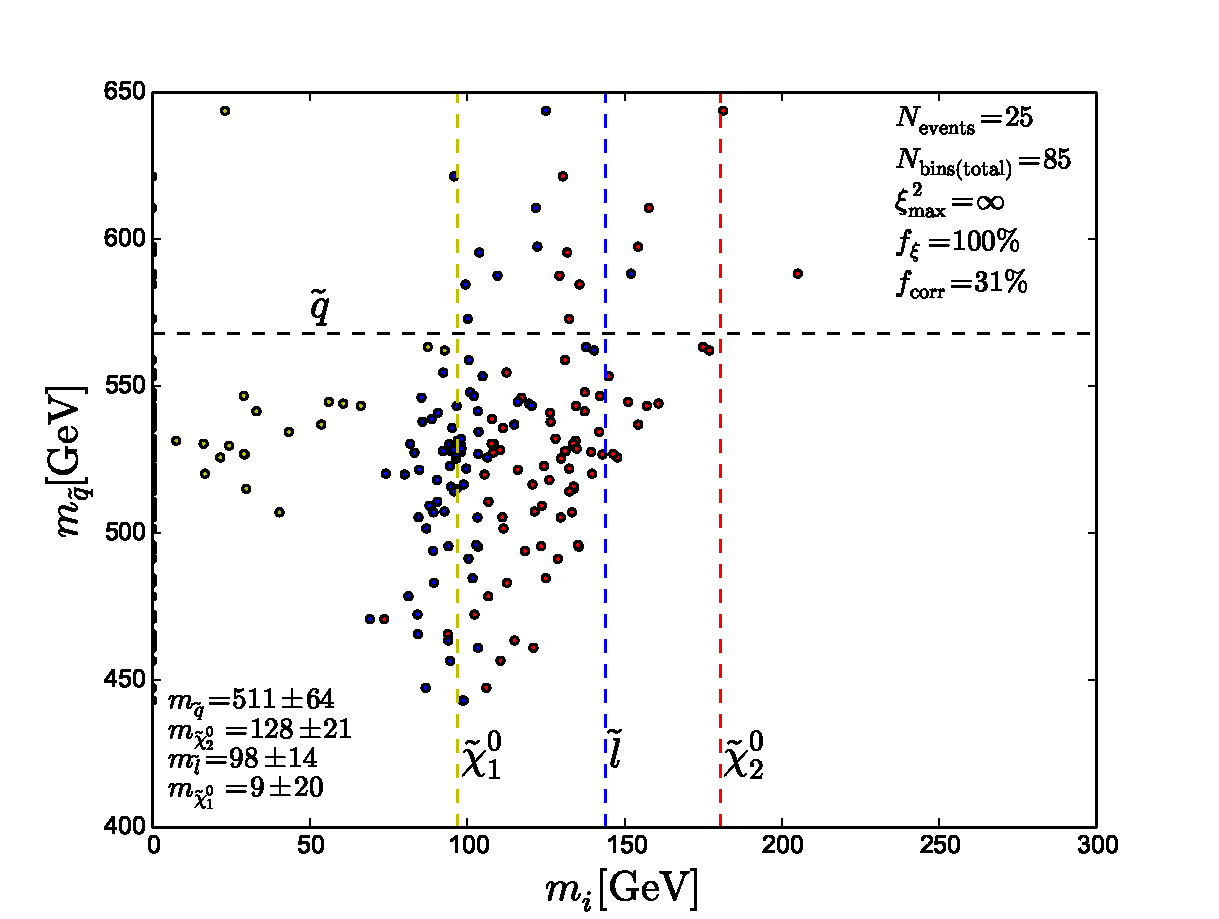
\includegraphics[width=\textwidth]{figures/webber_rec_table/webber-rec_wrong_starting_point-1000-100-80-30_lowtol.pdf}
		\caption{ } 
	\end{subfigure}
	\caption{Minimization on the unsmeared {\scshape HERWIG} dataset for different starting points: $\vec M = (568, 180, 144, 97)$ (the TMP) in {\bf (a)}, $\vec M = (400, 300, 200, 100)$  in {\bf (b)},$\vec M = (800, 500, 300, 50)$ in {\bf (c)} and $\vec M = (1000, 100, 80, 30)$ in {\bf (d)}.}
	\label{fig:starting_point_sensitivity_combinatorics}
\end{figure}

% The reason that we end up close to the true masses in most cases above is that we begin the search there. If we had started looking in some other more or less random point, we would not have gotten anywhere near as good results -- {\it because there is no minimum where we seem to have found it}. As an illustration, consider the scatter plot in figure \ref{fig:webber_rec_wrong_starting_point}, where the same dataset as above (without momentum smearing) is minimized with the same tolerance settings -- only we have started the search at the point $\vec M = (800, 500, 300, 50)$. There is no system in the points, and most of them end up outside the plotting region. 


It might however be that the function has multiple local minima, giving rise to the behaviour in figure \ref{fig:starting_point_sensitivity_combinatorics}, but that the {\it global} minimum is the one we find by starting in the TMP. To investigate this, we have made a scan of many starting points, minimizing the whole 100 bin dataset from each starting point. We selected five different values for each of the four SUSY masses and checked all combinations which make physical sense ({\it i.e.\ }where the mass hierarchy is present). This gave a total of 132 different starting points, which were indexed from 1 to 132. The TMP was point number 34. For each bin we then checked which index had the lowest $\xi^2$ value. Figure \ref{fig:webber_rec_hist_starting_points} shows a histogram of this. We see that number 34, the TMP, indeed dominates, but it is only the lowest in 14 of the 100 bins. The other 86 bins are distributed quite evenly among the other starting points. This leads us to conclude that the minimization, using this technique, simply is not well defined: There is no reasonable hope that we will be able to find a reliable best-fit estimate in an experimental situation where the TMP is unknown. This is especially true given that this scan was done on the unsmeared dataset -- we should expect even worse results when the resolution gets blurred by uncertainties.

\begin{figure}[hbt]
	\centering
	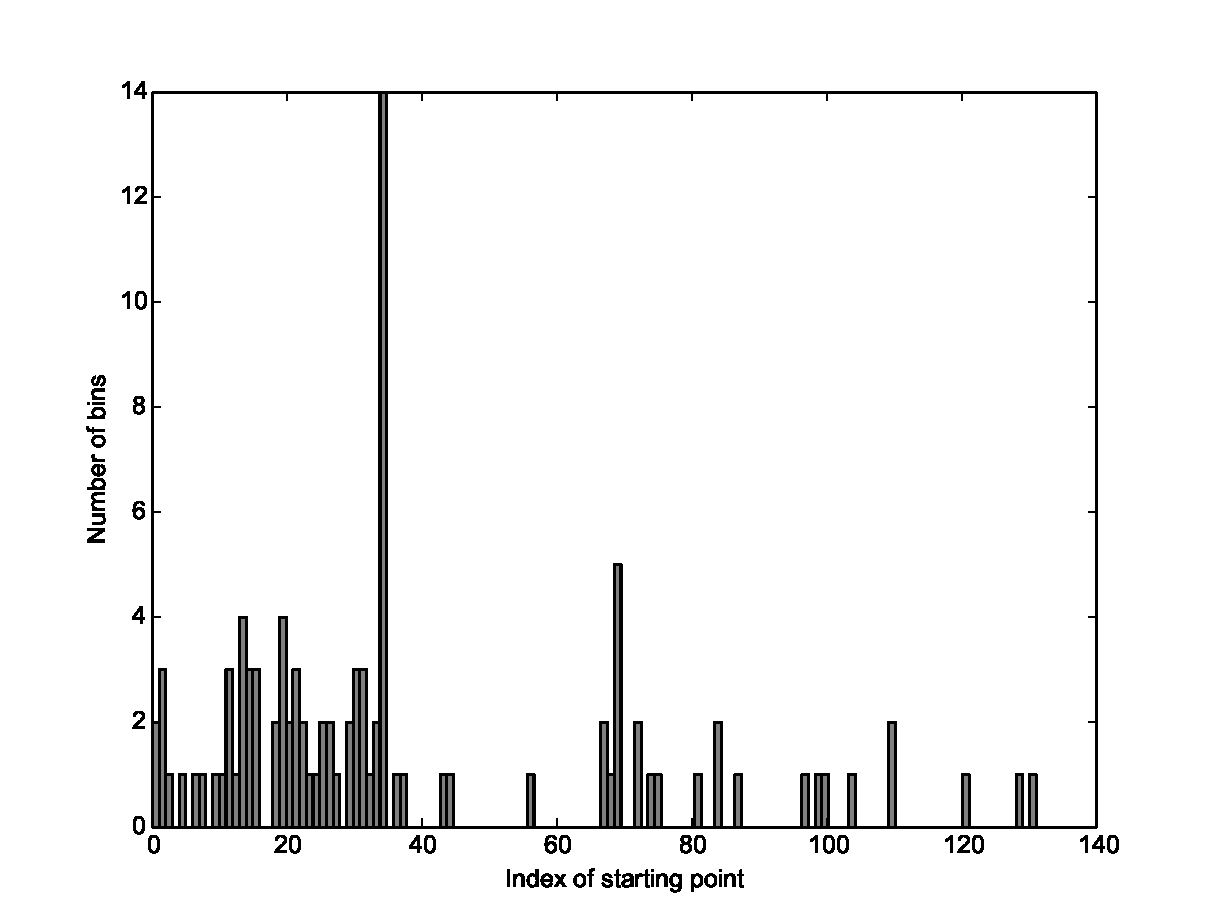
\includegraphics[width=0.8\textwidth]{figures/webber_rec_table/histogram_of_starting_points_with_lowest_minimal_value.pdf}
	\caption{A histogram of 100 data bins minimized from different starting points, showing distribution of lowest $\xi^2$ values. See the text for details.}
	\label{fig:webber_rec_hist_starting_points}
\end{figure}



% \begin{figure}[hbt]
% 	\centering
% 	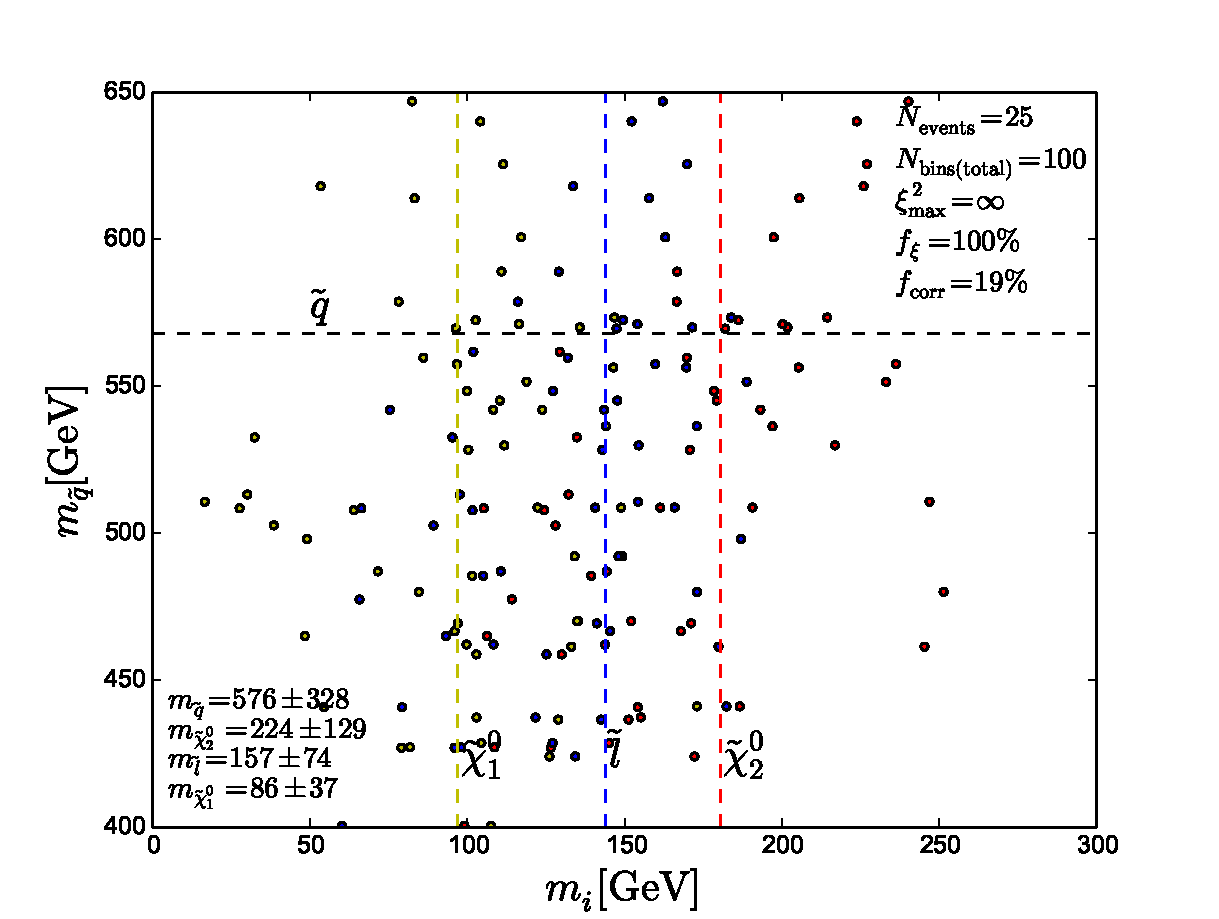
\includegraphics[width=0.8\textwidth]{figures/webber_rec_table/wrong_starting_point.pdf} 
% 	\caption{Minimization with the same tolerance as was used to produce table \ref{table:webber_rec}, but started far from the true mass point.}
% 	\label{fig:webber_rec_wrong_starting_point}
% \end{figure}




\clearpage






\section{Investigating improvements}
The objective of this thesis is to investigate and {\it improve} Webber's method. Having shown that there are problematic issues with Webber's demonstration of the method, we seem to be at odds with this goal. We have to try to pick up the pieces: Given that we from now on do a proper minimization ({\it i.e.\ } use a low enough tolerance), what can we hope to get out of the method? 

% The first thing to check is that choosing a proper tolerance in fact gives meaningful results when we begin the minimization at other points than the true mass values. If it does not, then we may dealing with a function that has no well-defined minimum -- which might well be the case, since we have included combinatorics, making the relatively simple polynomial of eq. \eqref{eq:xisquared} into something much more complicated. (The polynomial itself, being fourth order in each of the squared masses, can have only a limited number of local minima and should have a well-defined global one.) 

% And we do seem to be in trouble, because the minimization performance depends heavily on the choice of starting point. Figure \ref{fig:moving_on-starting_point_sensitivity_combinatorics} shows the minimization on the Herwig++ dataset, with combinatorics, for four different starting points. Subfigure {\bf (a)} is the true mass point, the other three are chosen somewhat randomly both over and under the true values. In all cases, the tolerance is set very low ($10^-12$) and the maximal number of iterations accepted is 500.

We saw in the previous section that the minimization was not well-defined, since it depended heavily on the choice of starting point. This was however a minimization done with the full inclusion of combinatorical ambiguities (see section \ref{sec:combinatorics}). While these ambiguities are clearly unavoidable -- we do not know \`{a} priori which particles belong together -- there may be other ways to handle them than the crude method applied in the above analysis. For one thing, it may be possible to rule out certain combinations based on phase-space cuts -- if there is a large mass hierarchy between {\it e.g.} the squark and its daughter, then the subsequent chain will be quite colinear, thus possibly ruling out combinations with large angles between momenta. It might also be possible to use other kinematical constraints, like the end-point method mentioned in section \ref{chap:introducing_the_method}, to rule out combinations. 

% \begin{figure}[hbt]
% 	\centering
% 	\begin{subfigure}[b]{0.45\textwidth}
% 		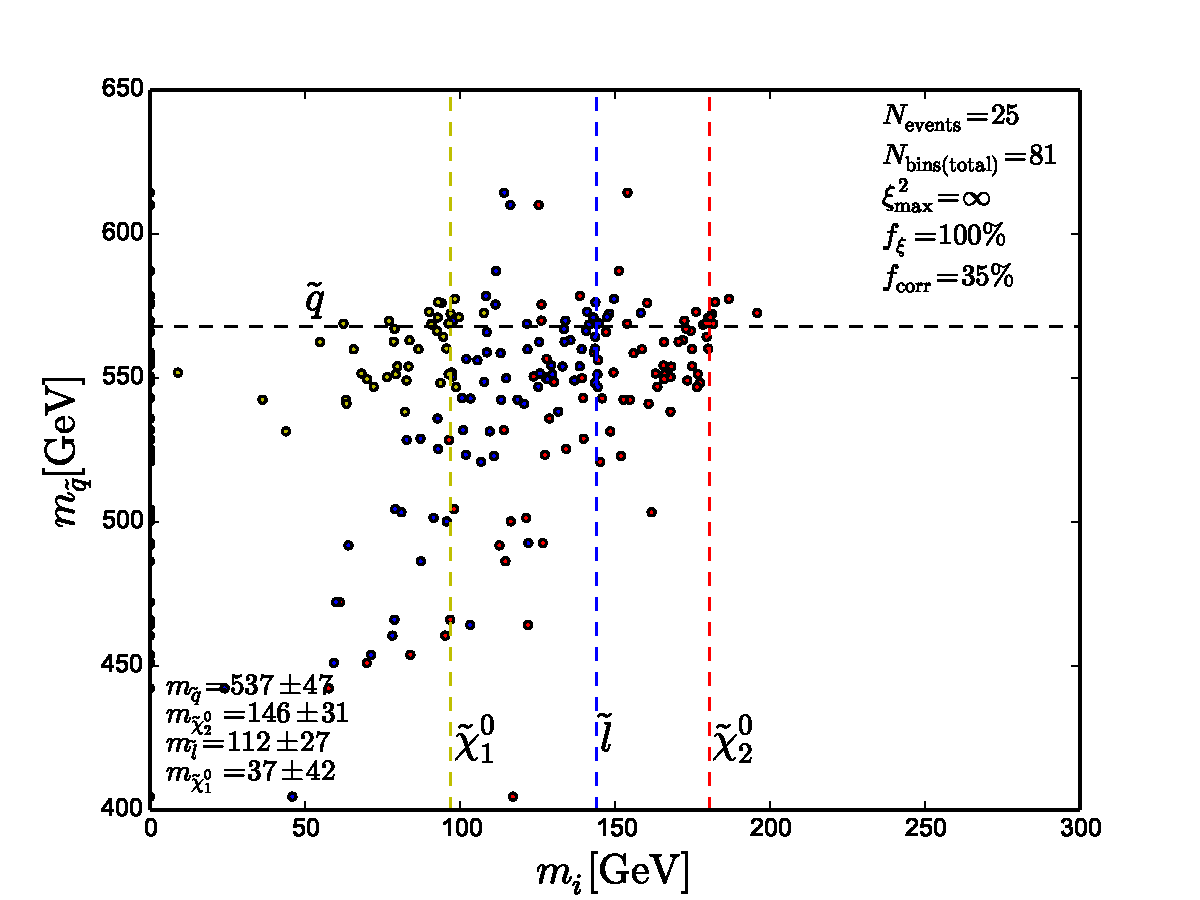
\includegraphics[width=\textwidth]{figures/moving_on/herwig-568-180-144-97-maxiter500-comb-nocut.pdf} 
% 		\caption{ }
% 	\end{subfigure}
% 	\begin{subfigure}[b]{0.45\textwidth}
% 		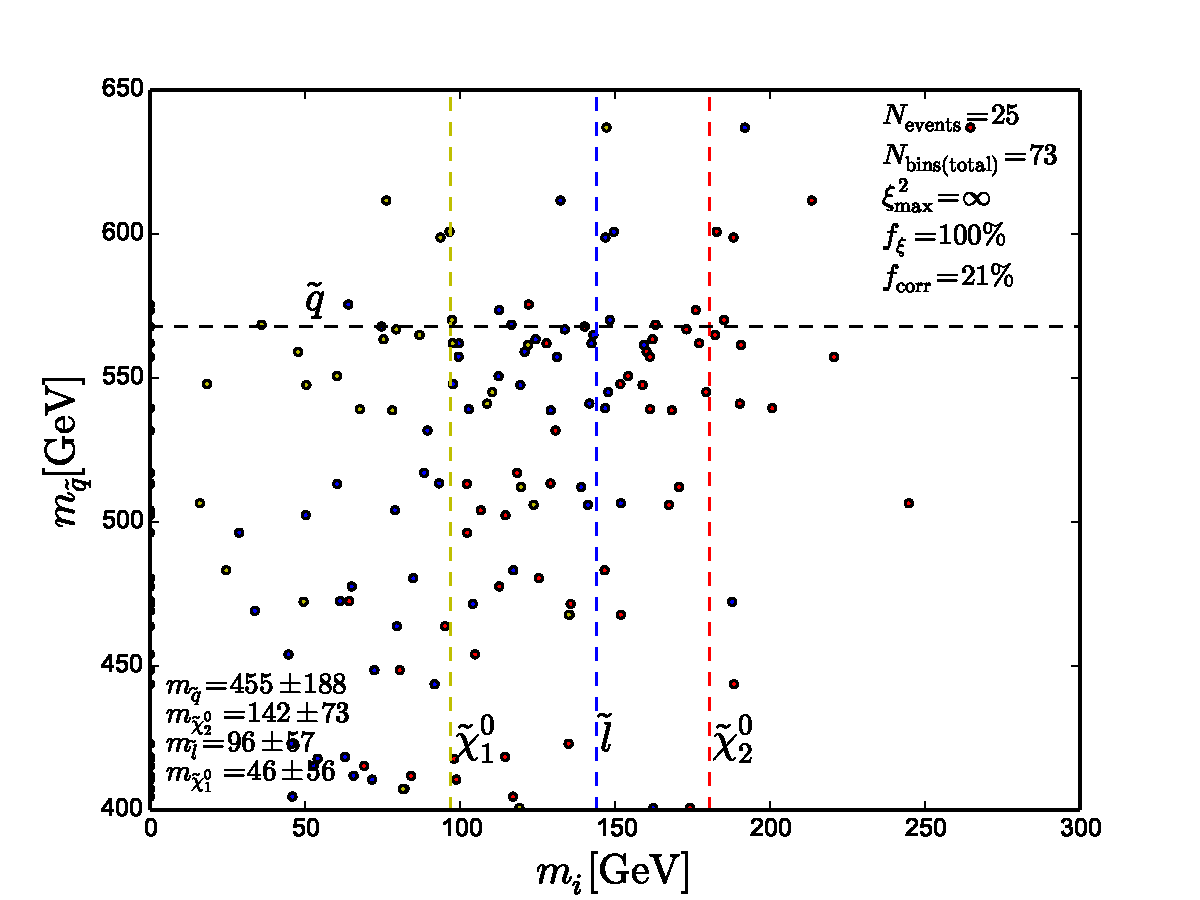
\includegraphics[width=\textwidth]{figures/moving_on/herwig-800-500-300-50-maxiter500-comb-nocut.pdf}
% 		\caption{ } 
% 	\end{subfigure}

% 	\begin{subfigure}[b]{0.45\textwidth}
% 		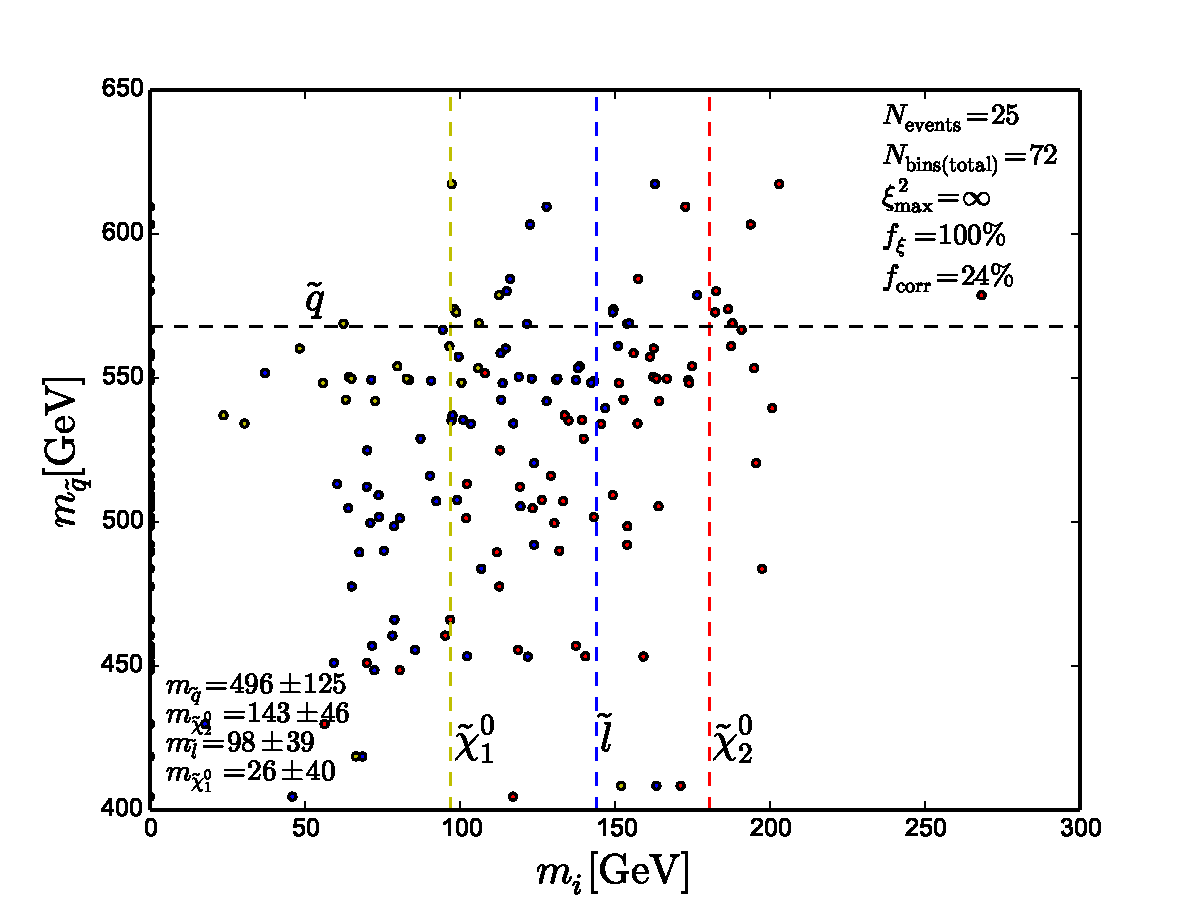
\includegraphics[width=\textwidth]{figures/moving_on/herwig-400-300-200-100-maxiter500-comb-nocut.pdf} 
% 		\caption{ }
% 	\end{subfigure}
% 	\begin{subfigure}[b]{0.45\textwidth}
% 		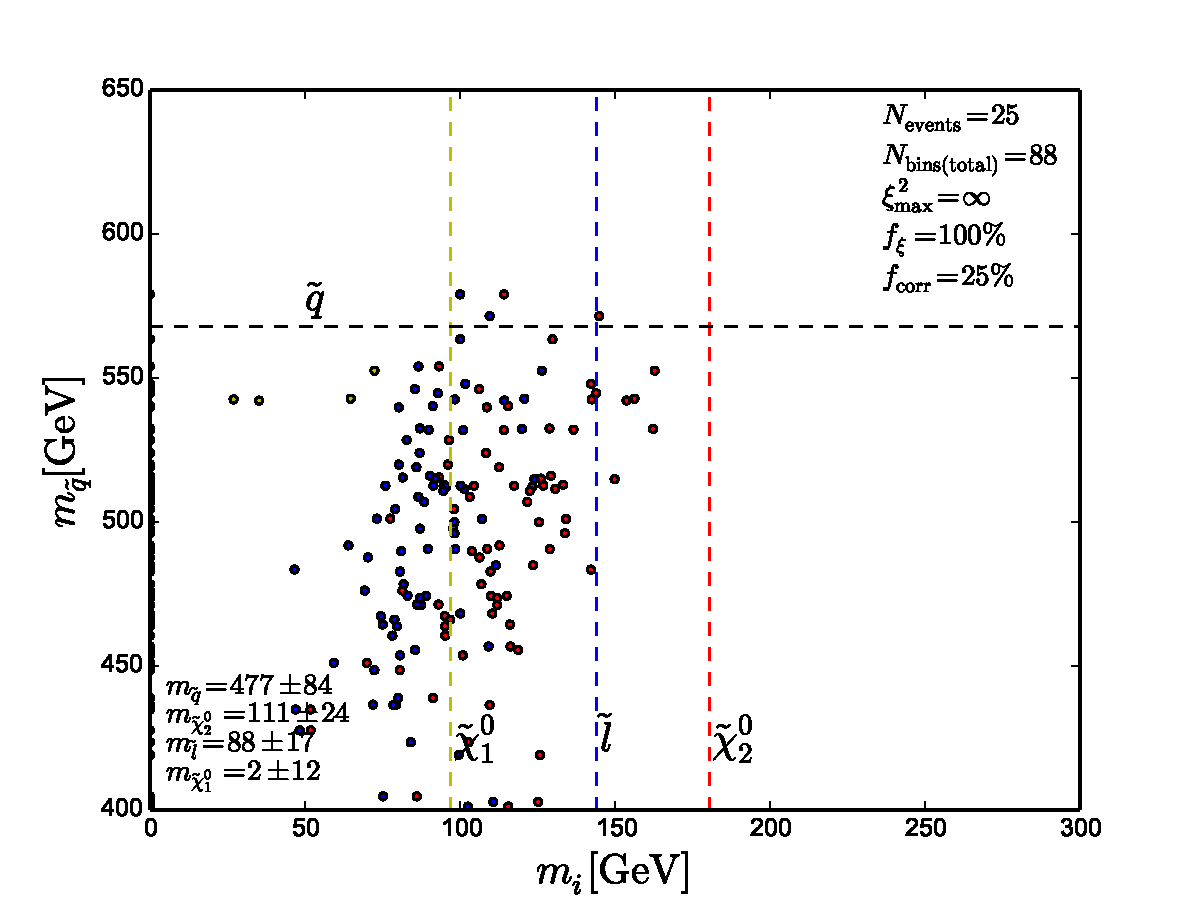
\includegraphics[width=\textwidth]{figures/moving_on/herwig-1000-100-80-30-maxiter500-comb-nocut.pdf}
% 		\caption{ } 
% 	\end{subfigure}
% 	\caption{Minimization on the same dataset for different starting points: $\vec M = (568, 180, 144, 97)$ (the true mass point) in {\bf (a)}, $\vec M = (800, 500, 300, 50)$ in {\bf (b)}, $\vec M = (400, 300, 200, 100)$ in {\bf (c)} and $\vec M = (1000, 100, 80, 30)$ in {\bf (d)}.}
% 	\label{fig:moving_on-starting_point_sensitivity_combinatorics}
% \end{figure}

% This clearly does not work. The minimization does not find starting point-independent best-fit points. This means that the minimization problem is unsolvable. This may either indicate that the function is flat ({\it i.e.\ } the minimum is highly degenerate), that it has multiple local minima (they are highly non-trivial to classify because the function is so compliated) or that the Simplex method just cannot handle this problem ({\it e.g.\ } because the function is non-smooth). In any case, we must look for another approach.




\subsection{What can be salvaged}

There may still be hope, however. If we for a moment forget about the combinatorics, and evaluate only the true particle combination for each event, then the minimization is well-defined. This is illustrated in figure \ref{fig:starting_point_sensitivity_no_combinatorics}, which shows minimization of 100 samples of 25 events minimized with low tolerance, but only evaluated with the correct combination of chain particles.\footnote{This dataset is generated with {\scshape Herwig++} version 2.7.1 \cite{Bahr:2008pv} and minimized using our own implementation of the {\scshape Simplex} algorithm in C++. We have made thorough checks that this gives identical results with the Fortran {\scshape HERWIG} program used above.} There are discrepancies between the fits, mainly between subfigure d and the others. In particular, while about 85 of the samples converge within the set limit of 500 iterations in each of the cases a, b and c (indicated by the value of $N_\mathrm{bins(total)}$ in the top right of each plot), this number is reduced to 67 in subfigure d. The starting point in case (d) is characterized by a much larger mass gap between the squark and the $\tilde\chi_2^0$ than in the TMP, which we might surmise would give rise to very different kinematics than we have in our events. In any case, the minimization is not a heavy calculation (the whole minimization of 100 bins, including combinatorics, is done in fractions of a second on a single CPU core), so doing a scan like the one we made above over different starting points is not unrealistic. 


% , but this appears to mainly concern the outlying points, where the fit is bad anyway, and which we might hope to remove by a cut on the $\xi^2$. The main clusters of points are fitted the same in all four cases, which shows that they are in fact real and well-defined best-fit points. 


\begin{figure}[hbt]
	\centering
	\begin{subfigure}[b]{0.45\textwidth}
		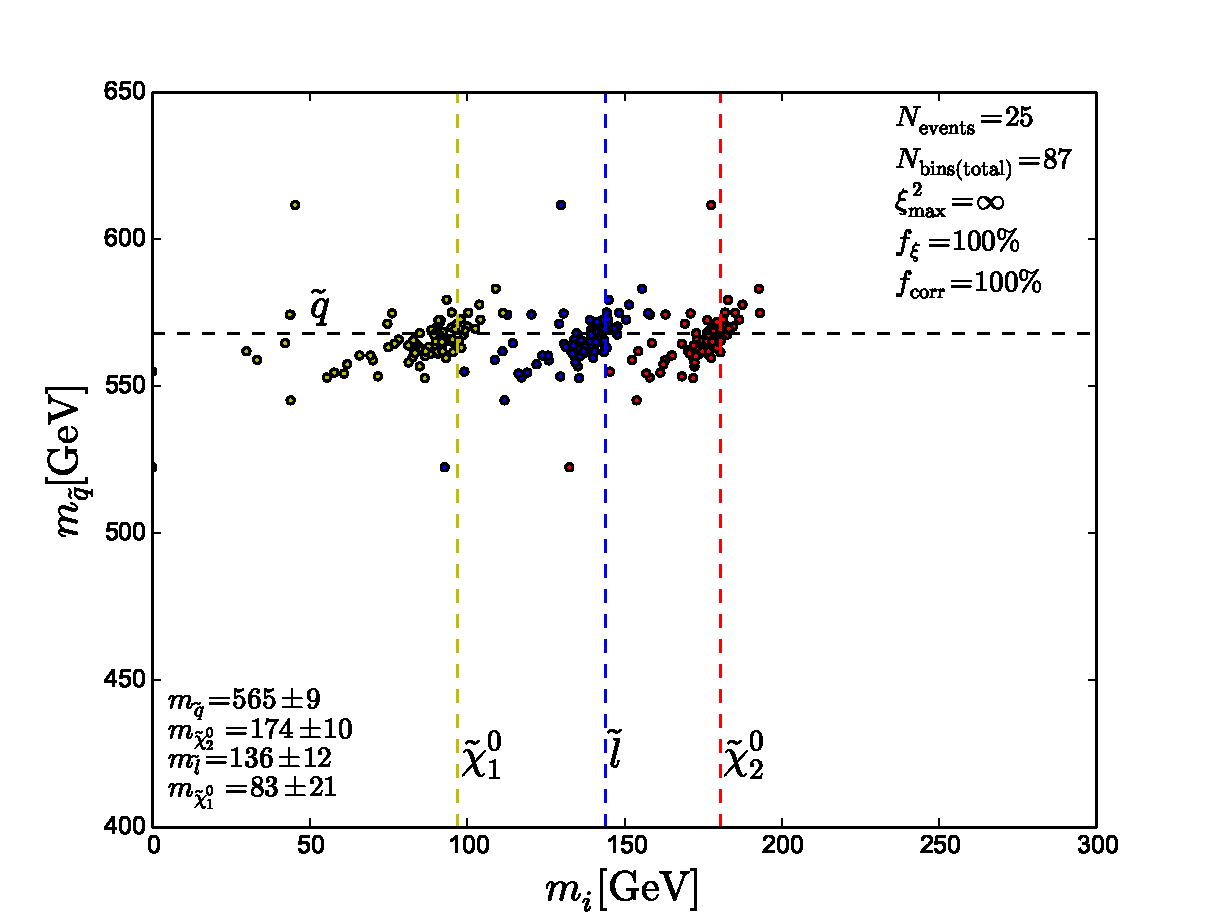
\includegraphics[width=\textwidth]{figures/improving_combinatorics/herwigpp-momcons_nocomb_truemasspoint.pdf} 
		\caption{ }
	\end{subfigure}
	\begin{subfigure}[b]{0.45\textwidth}
		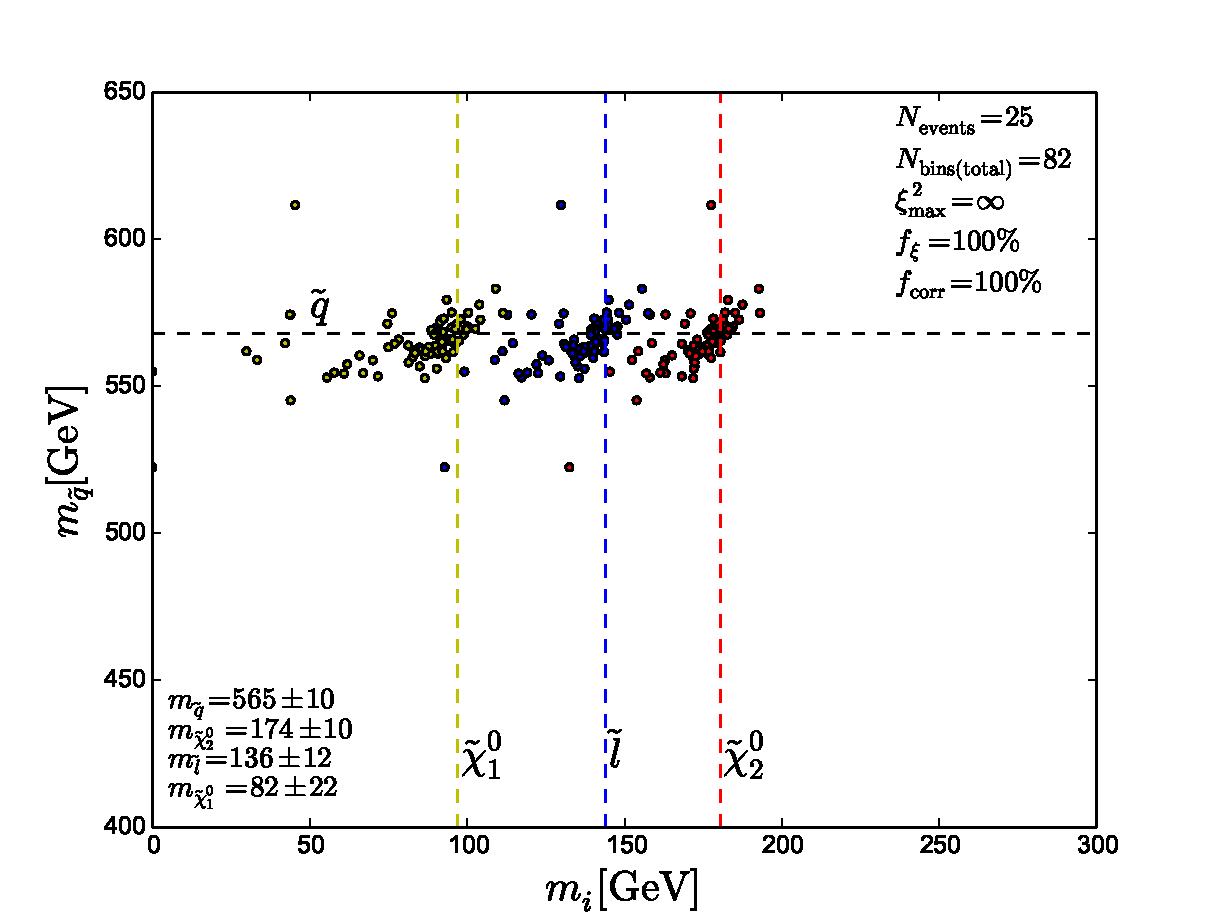
\includegraphics[width=\textwidth]{figures/improving_combinatorics/herwigpp-momcons_nocomb_400-300-200-100.pdf}
		\caption{ } 
	\end{subfigure}

	\begin{subfigure}[b]{0.45\textwidth}
		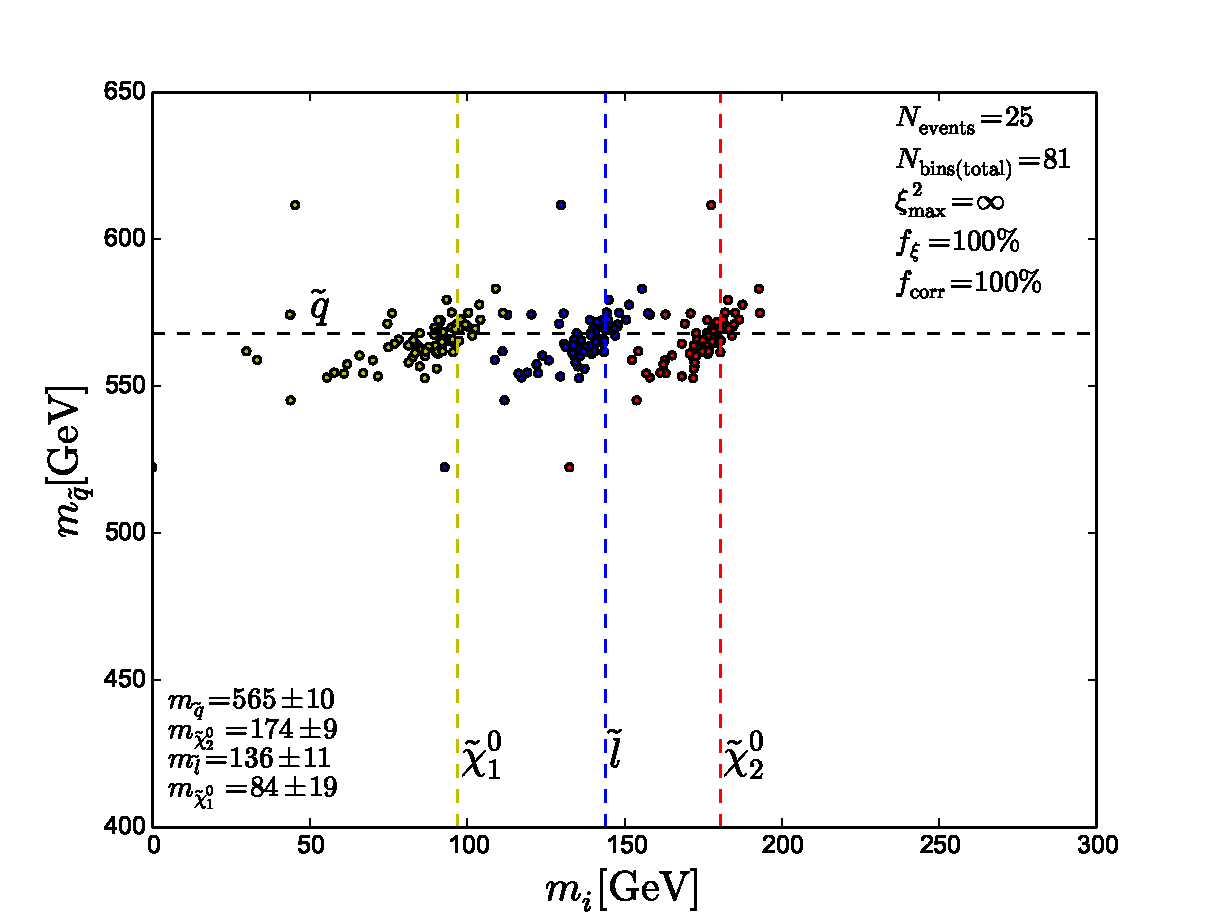
\includegraphics[width=\textwidth]{figures/improving_combinatorics/herwigpp-momcons_nocomb_800-500-300-50.pdf} 
		\caption{ }
	\end{subfigure}
	\begin{subfigure}[b]{0.45\textwidth}
		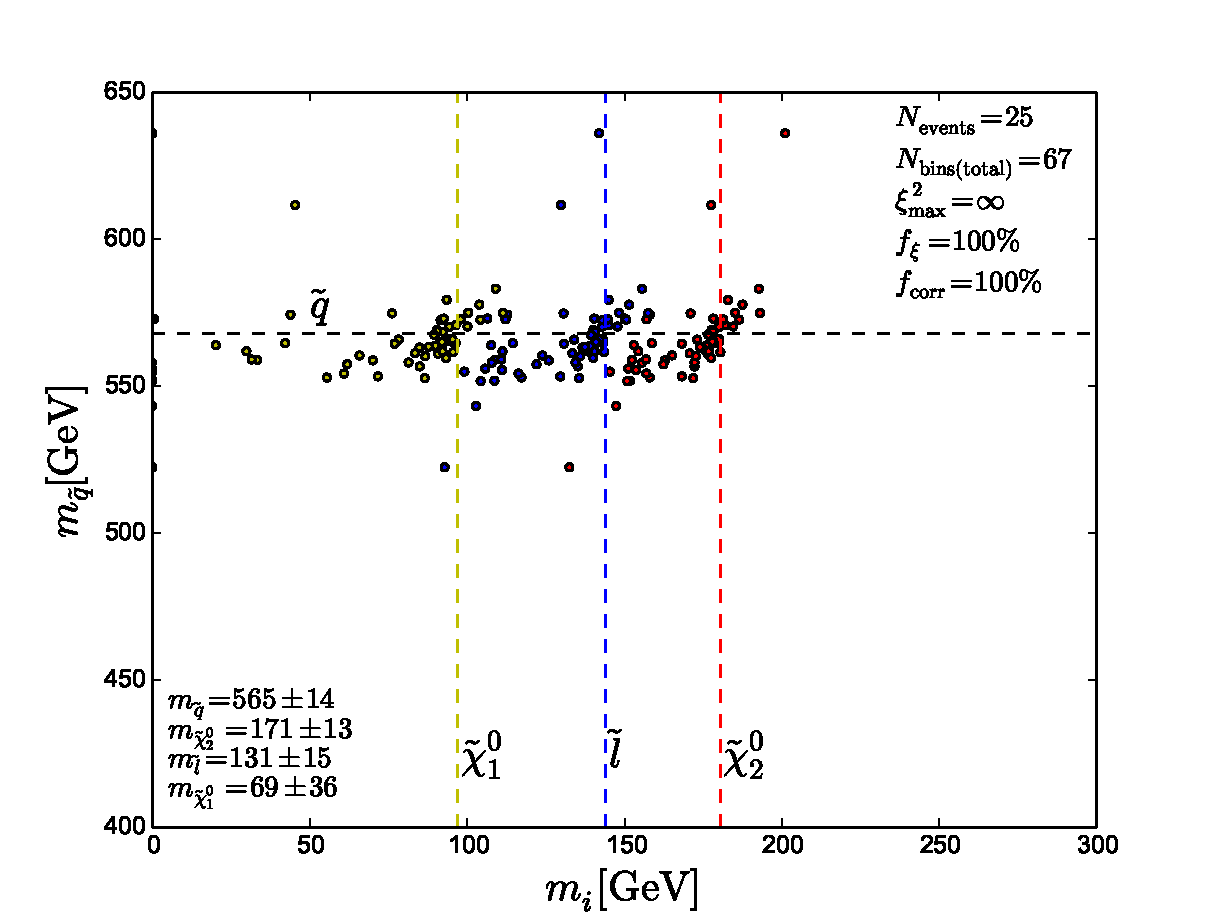
\includegraphics[width=\textwidth]{figures/improving_combinatorics/herwigpp-momcons_nocomb_1000-100-80-30.pdf}
		\caption{ } 
	\end{subfigure}
	\caption{An equivalent fit to figure \ref{fig:starting_point_sensitivity_combinatorics} (on a {\ttfamily Herwig++} dataset), but the $\xi^2$ contribution is only evaluated for the true particle combination in each event.}
	\label{fig:moving_on-starting_point_sensitivity_no_combinatorics}
\end{figure}

% \begin{figure}[hbt]
% 	\centering
% 	\begin{subfigure}[b]{0.45\textwidth}
% 		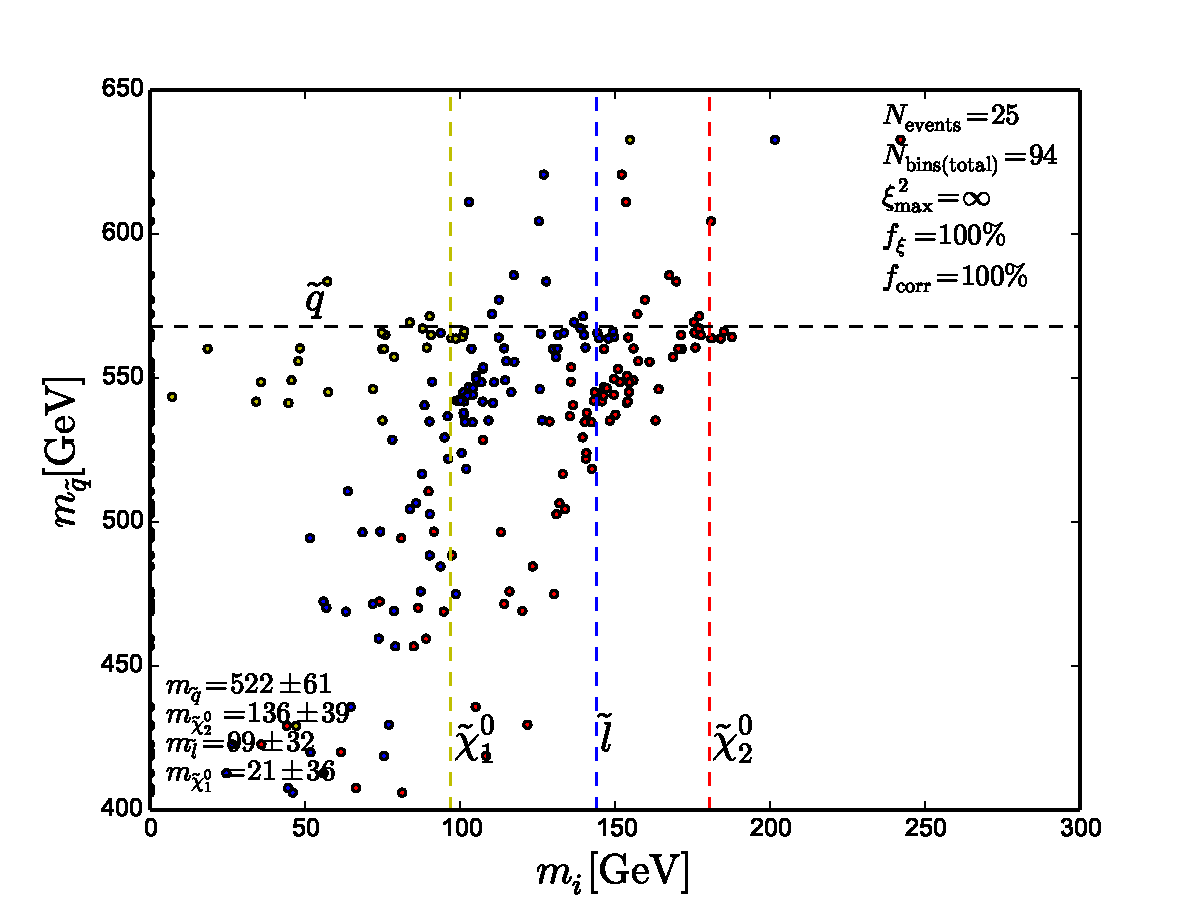
\includegraphics[width=\textwidth]{figures/moving_on/herwig-568-180-144-97-maxiter1000-nocomb-nocut.pdf} 
% 		\caption{ }
% 	\end{subfigure}
% 	\begin{subfigure}[b]{0.45\textwidth}
% 		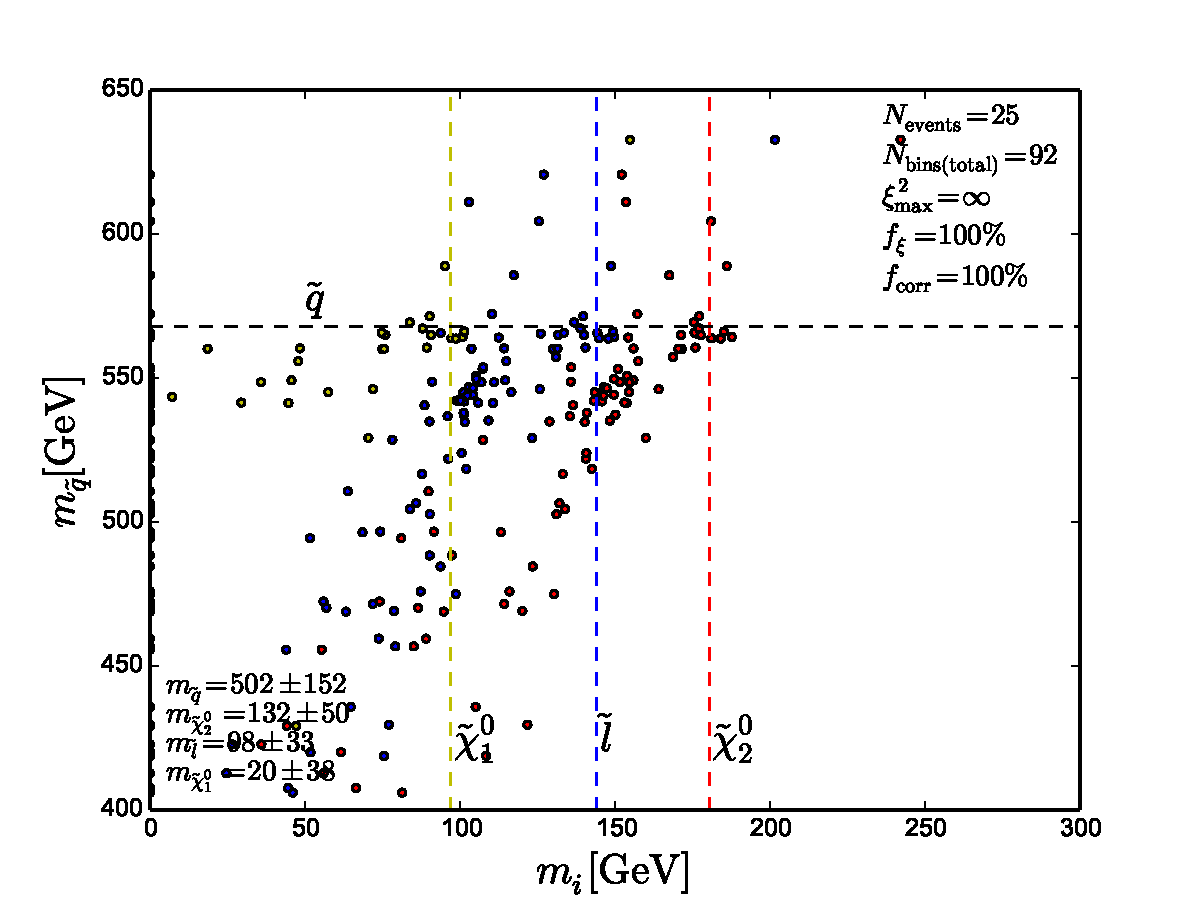
\includegraphics[width=\textwidth]{figures/moving_on/herwig-800-500-300-50-maxiter1000-nocomb-nocut.pdf}
% 		\caption{ } 
% 	\end{subfigure}

% 	\begin{subfigure}[b]{0.45\textwidth}
% 		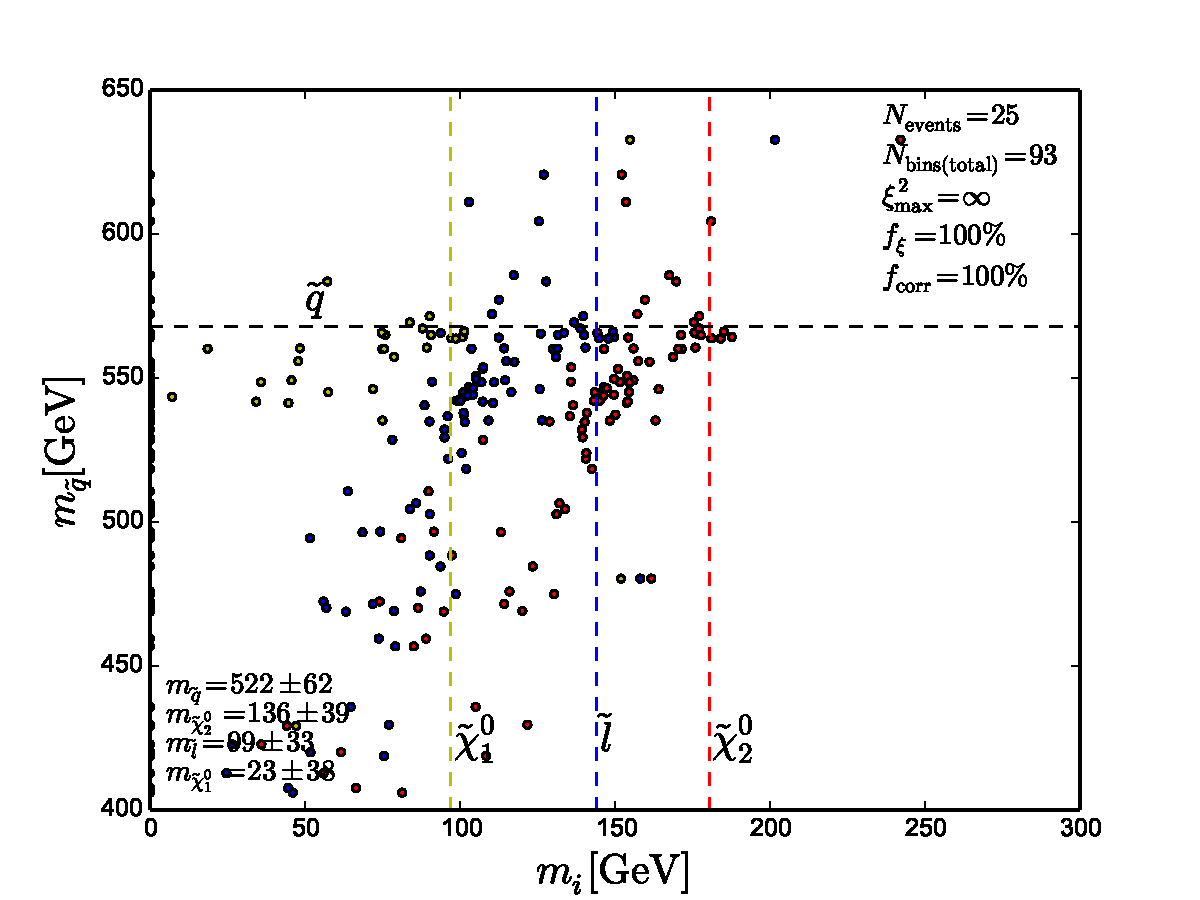
\includegraphics[width=\textwidth]{figures/moving_on/herwig-400-300-200-100-maxiter1000-nocomb-nocut.pdf} 
% 		\caption{ }
% 	\end{subfigure}
% 	\begin{subfigure}[b]{0.45\textwidth}
% 		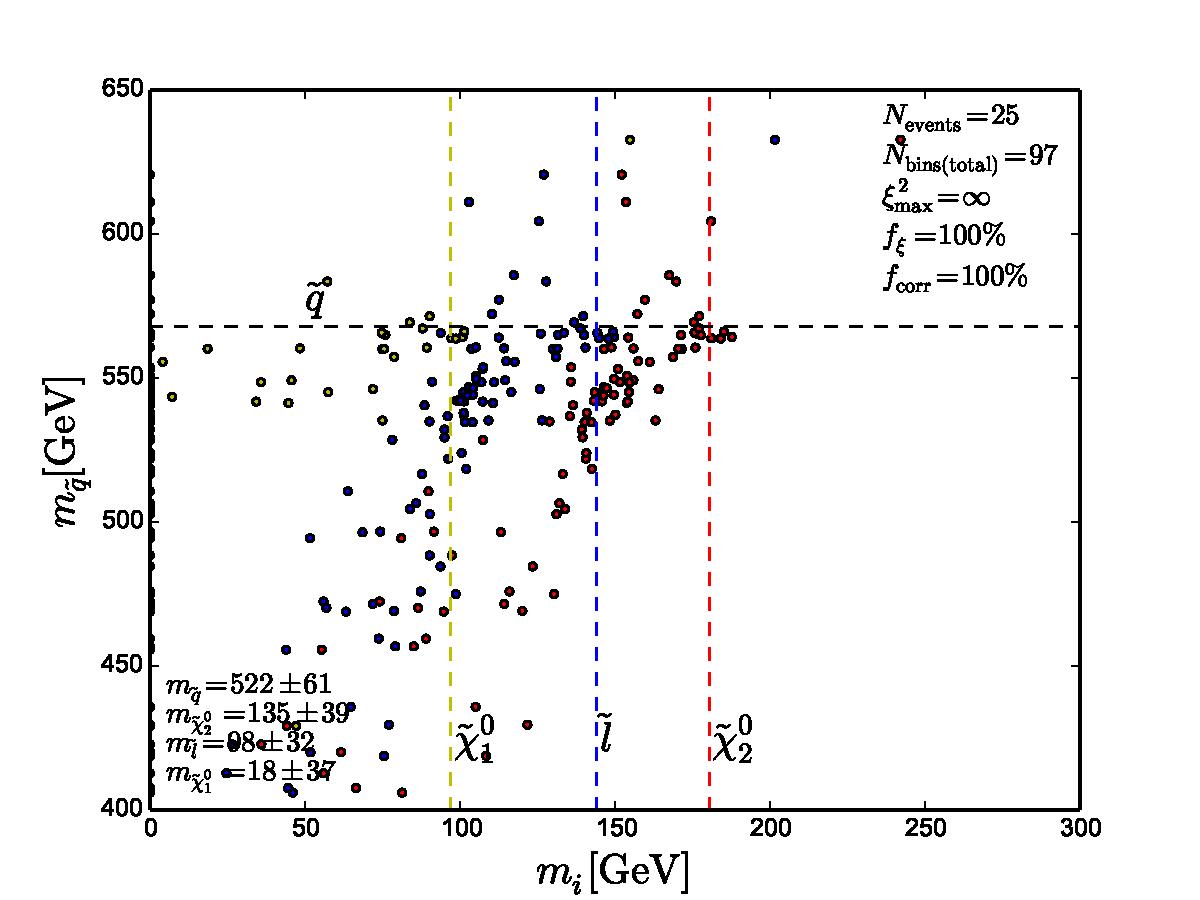
\includegraphics[width=\textwidth]{figures/moving_on/herwig-1000-100-80-30-maxiter1000-nocomb-nocut.pdf}
% 		\caption{ } 
% 	\end{subfigure}
% 	\caption{The same fit as in figure \ref{fig:moving_on-starting_point_sensitivity_combinatorics}, but without taking combinatorics into account.}
% 	\label{fig:moving_on-starting_point_sensitivity_no_combinatorics}
% \end{figure}

We also keep in mind the effects of momentum smearing, and check the no-combinatorics minimization on the 10 \% smeared dataset for the same four starting points.The plots are shown in figure \ref{fig:moving_on-starting_point_sensitivity_no_combinatorics_10pmomsmear}. We find that it indeed is a well-defined minimization -- but the LSP mass is fitted to zero! It appears that when the data is smeared, the method loses its sensitivity to the LSP mass. Or equivalently, we could say that it loses its sensitivity to {\it the absolute mass scale} of the problem. This is a well-known problem with methods for mass reconstruction -- in the Standard Model, the masses of the neutrinos are not known, only the mass-square difference. 

\begin{figure}[hbt]
	\centering
	\begin{subfigure}[b]{0.45\textwidth}
		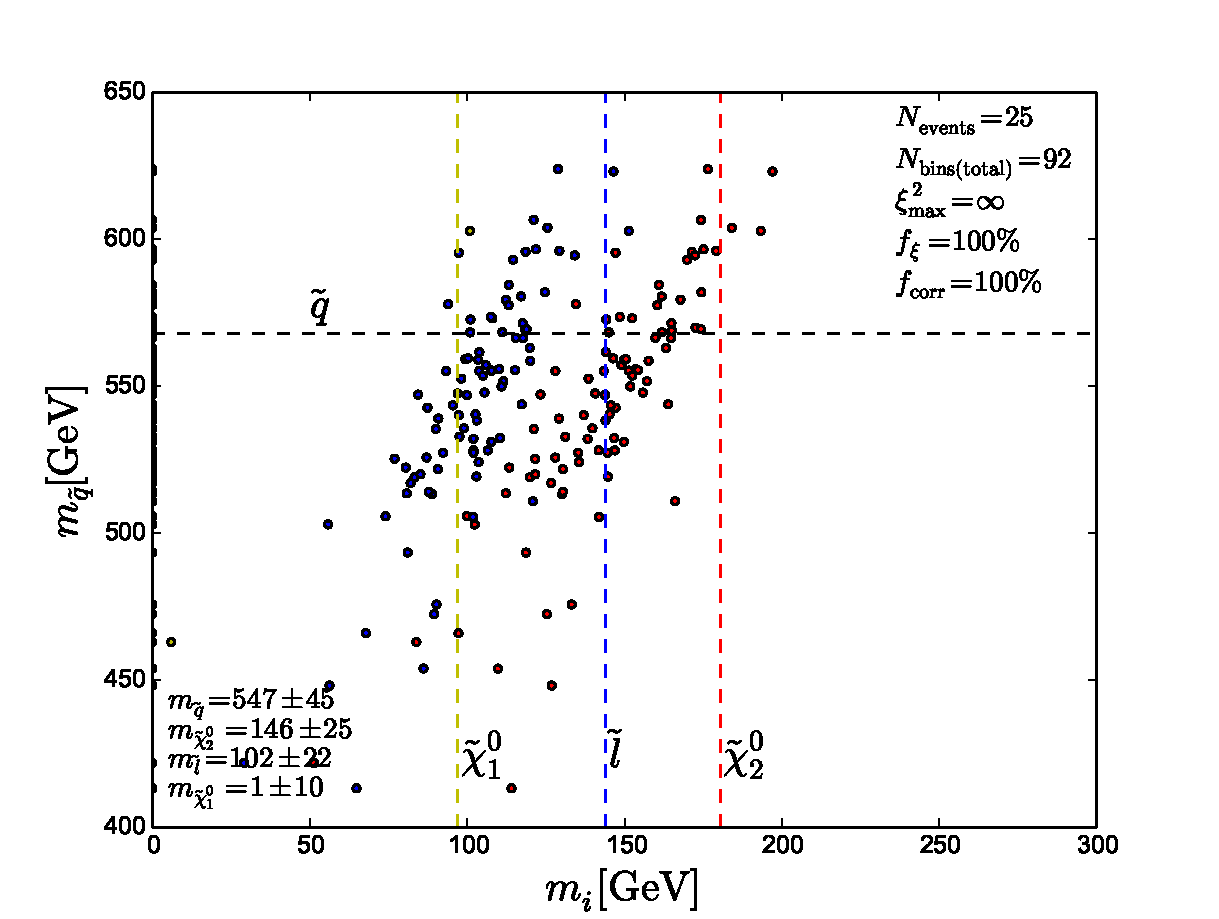
\includegraphics[width=\textwidth]{figures/improving_combinatorics/herwigpp_10psmear_lowtol_nocomb_TMP.pdf} 
		\caption{ }
	\end{subfigure}
	\begin{subfigure}[b]{0.45\textwidth}
		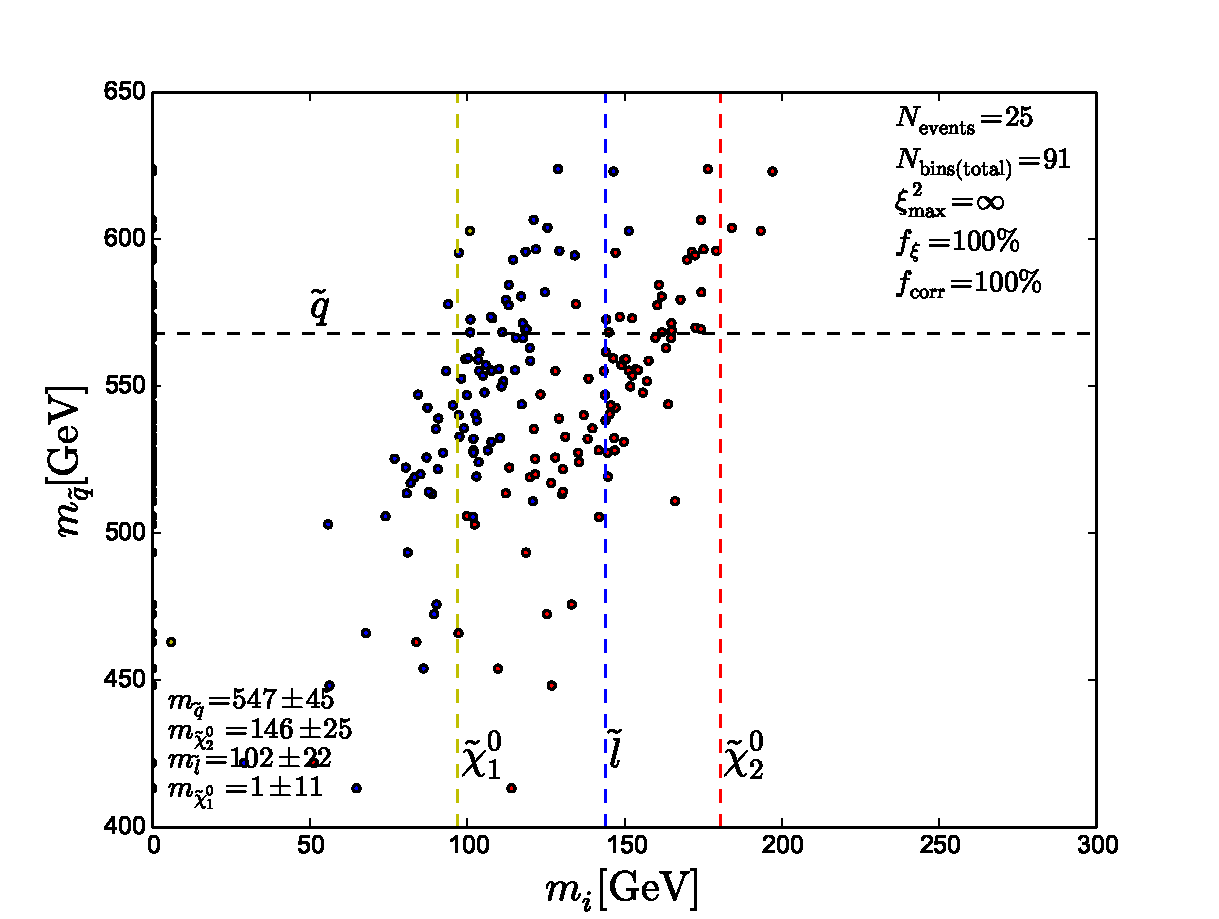
\includegraphics[width=\textwidth]{figures/improving_combinatorics/herwigpp_10psmear_lowtol_nocomb_400-300-200-100.pdf}
		\caption{ } 
	\end{subfigure}

	\begin{subfigure}[b]{0.45\textwidth}
		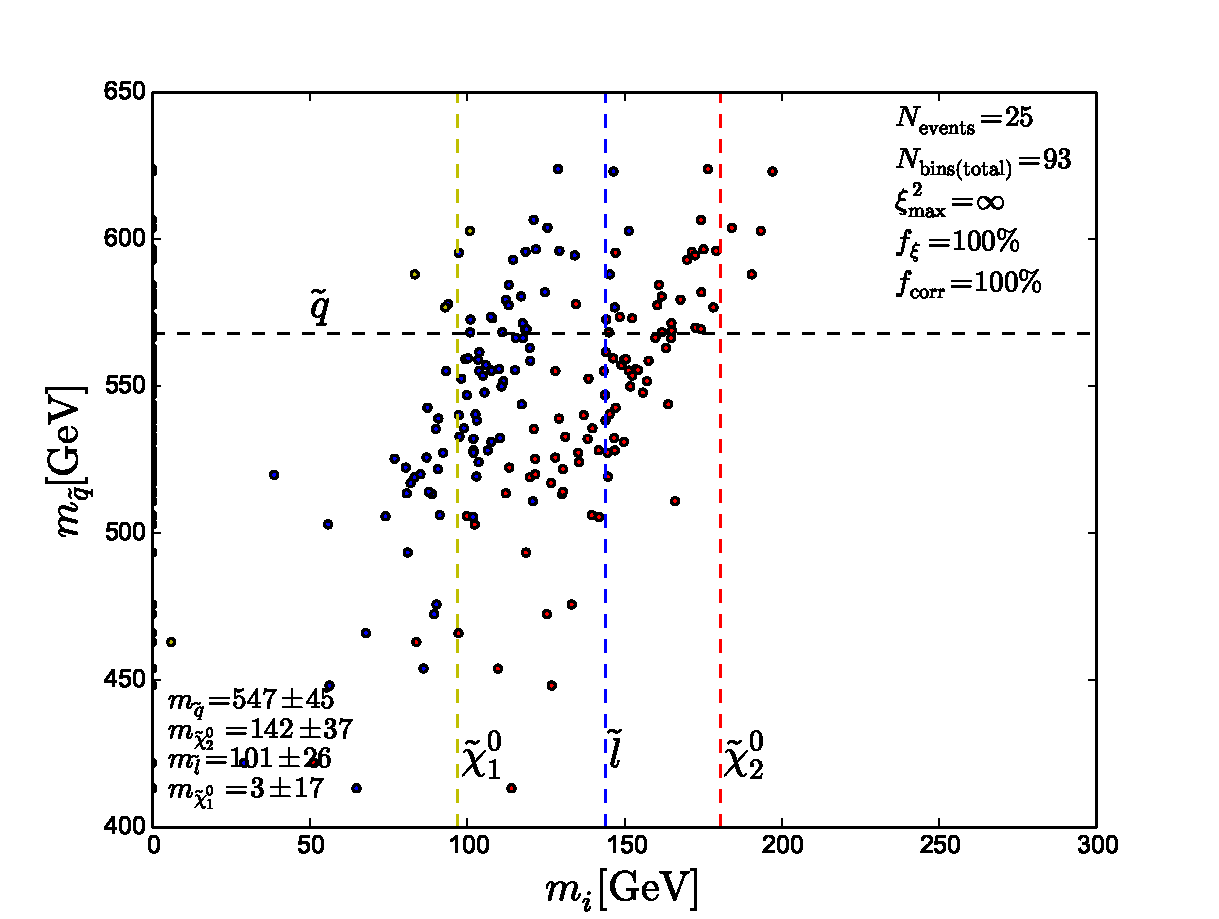
\includegraphics[width=\textwidth]{figures/improving_combinatorics/herwigpp_10psmear_lowtol_nocomb_800-500-300-50.pdf} 
		\caption{ }
	\end{subfigure}
	\begin{subfigure}[b]{0.45\textwidth}
		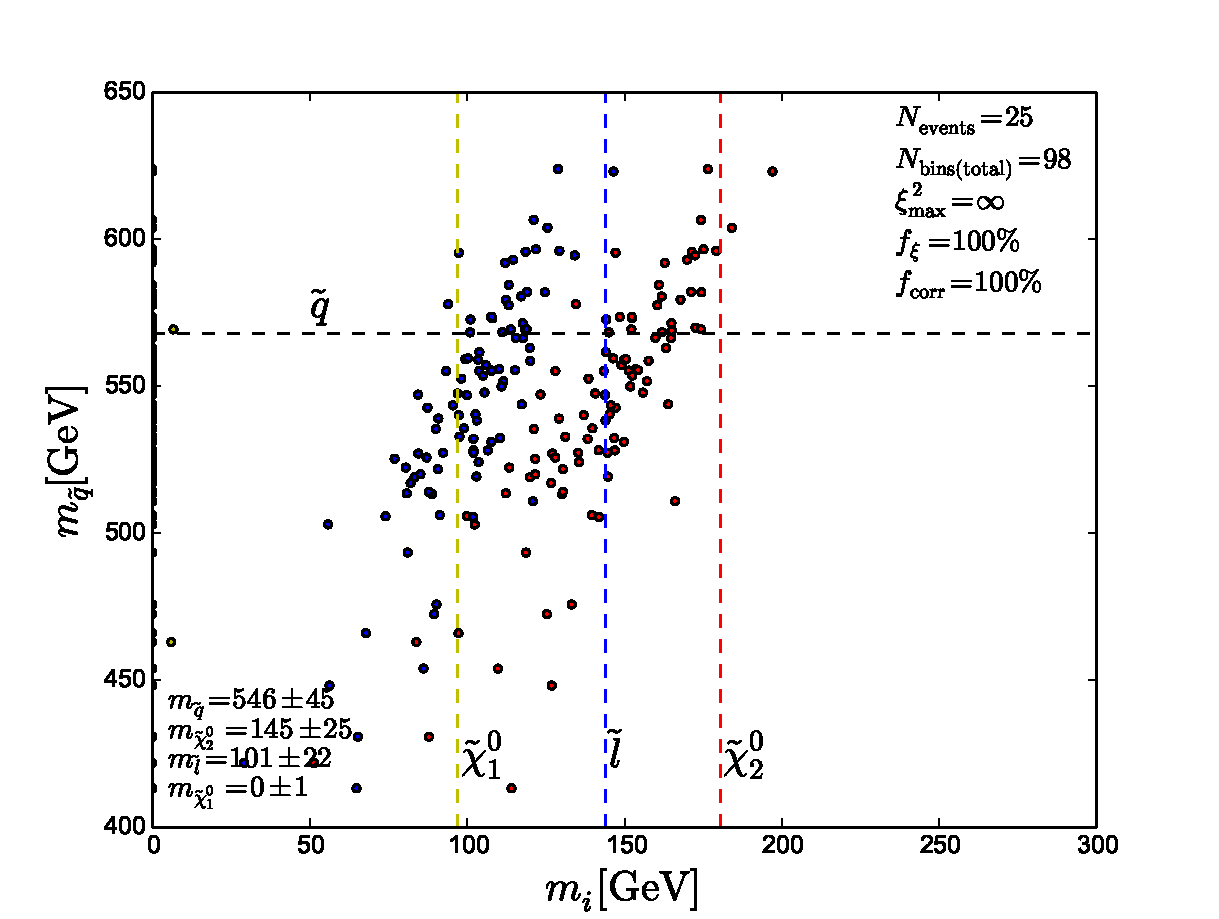
\includegraphics[width=\textwidth]{figures/improving_combinatorics/herwigpp_10psmear_lowtol_nocomb_1000-100-80-30.pdf}
		\caption{ } 
	\end{subfigure}
	\caption{Again the same fit as in \ref{fig:starting_point_sensitivity_combinatorics} and \ref{fig:moving_on-starting_point_sensitivity_no_combinatorics}, here with a 10 \% smeared dataset and no combinatorics.}
	\label{fig:moving_on-starting_point_sensitivity_no_combinatorics_10pmomsmear}
\end{figure}


Of course, we still have to take the combinatorical ambiguities into account. But the approach where we evaluate all combinations at each point to determine the kinematically best combination, as outlined in section \ref{sec:combinatorics}, seems to be useless. 
% What if we instead minimize the $\xi^2$ for each {\it event} separately, for all 






\begin{itemize}
	\item Minimize separately for each event? Do something to make it steep enough?
	\item combinatorical elimination: momentum cuts, angles, invariant mass edge. Angular selection: squarks produced more or less at rest (except if they come from gluino in a large mass-gap scenario). But if there is a mass gap further down, does this give anisotropies in angular distributions of opposite-chain particles?
	\item migrad or similar for minimization of 1-event bins? Provide gradient, analytical or numerical?
	\item combinatorical issues with three or four hard squarks -- gluino-gluino vs gluino-squark vs squark-squark/squark-antisquark. Nllfast to give xsec. 
\end{itemize}



















% \chapter{OLD version of MC chapter}

% \section{Production mechanisms}
% There are several ways in which a pair of squarks can be produced in $pp$ collisions. Figure \ref{fig:squark_production_diagrams} shows Feynman diagrams of different processes that contribute.\footnote{The diagrams are made using JaxoDraw \cite{Binosi:2003yf}.} In (a) and (c) the squarks are opposite sign and in (a) also same flavour, while in (b) and (d) we have no such guarantee. Additionally, in (b) and (d) the squarks are produced along with additional quarks.\marginpar{If this is kept, make sure to include all diagrams from article.}

% \begin{figure}[hbt]
% 	\centering
% 	\begin{subfigure}[b]{0.4\textwidth}
% 		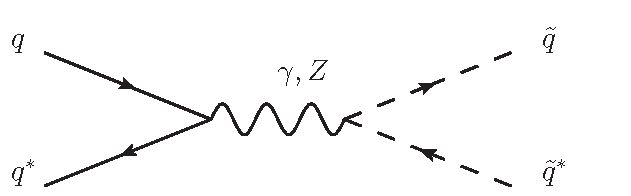
\includegraphics[width=\textwidth]{figures/qqbar_to_tildeqqbar_s_channel.pdf} 
% 		\caption{ }
% 	\end{subfigure}
% 	\begin{subfigure}[b]{0.4\textwidth}
% 		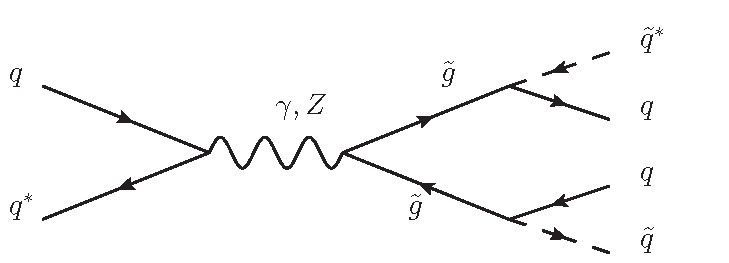
\includegraphics[width=\textwidth]{figures/qqbar_to_gluinos_to_qqtildeqq_s_channel.pdf}
% 		\caption{ } 
% 	\end{subfigure}

% 	\begin{subfigure}[b]{0.4\textwidth}
% 		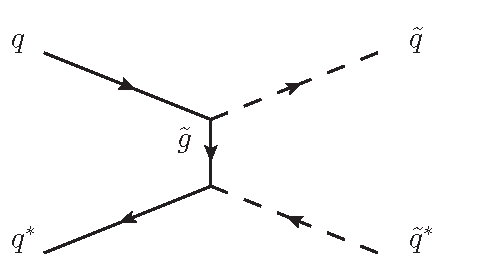
\includegraphics[width=\textwidth]{figures/qqbar_to_tildeqqbar.pdf} 
% 		\caption{ }
% 	\end{subfigure}
% 	\begin{subfigure}[b]{0.4\textwidth}
% 		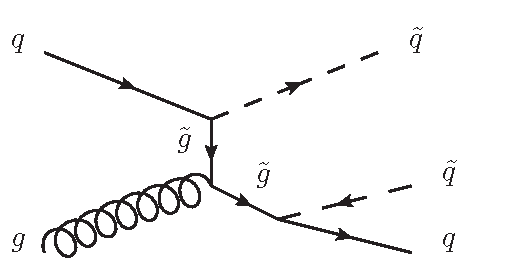
\includegraphics[width=\textwidth]{figures/qg_to_tildeqqbar.pdf}
% 		\caption{ } 
% 	\end{subfigure}
% 	\caption{Diagrams for squark pair production.}
% 	\label{fig:squark_production_diagrams}
% \end{figure}

% However, the production of additional quarks is irrelevant for the analysis and reconstruction of the cascade, because we only wish to reconstruct the chain back to the squark. So is the distinction between squark flavours. The only significance of the flavour of squark (apart from its mass, of course) is on the flavour of quark it decays to along with the $\chi_2^0$ -- the quark and squark must be of the same flavour and sign. The $\chi_2^0$ cannot transmit any information about the flavour of its squark mother, so the subsequent leptonic decay is independent of the previous history. The quark will hadronize to form a hadron jet, and the properties of this jet are in principle dependent on the type of quark. However, current detectors are not good at discriminating between quark flavours of the first two generations; it can only discover $b$ quarks using the technique of {\it b-tagging} and to some extent $c$ quarks via {\it c-tagging}. In our analysis we will veto events containing $b$ quarks as the mass splitting of the squarks between the first/second and third generation prevent a good fit with a single squark mass.



% \section{The simplest possible case: Squarks decaying at rest}
% The very simplest way to study this problem, when all the complications of reality are stripped away, consists of a pair of heavy particles which each decay in a series of on-shell two-body decays down to three light particles that are detected and one that escapes. This idealized situation constrains the possible performance of Webber's method on the most general level, so we choose to start here. To decay the particles we use the algorithm described in appendix \ref{ch:decayalgorithm}. The algorithm assumes that everything is completely on-shell, so there is no Breit-Wigner smearing of the unstable particle masses, no initial- or final state radiation of photons or gluons that could force particles off-shell and no loss of energy in the process.

% We take the CMMSM benchmark point SPS 1a \cite{Allanach:2002nj} as our mass parameter point. As mentioned above, we will only consider the first two generations of squarks. We will also take them to be left-handed, primarily since right-handed squarks have low cross-sections at SPS 1a (see discussion in the next section). The squarks we end up studying are then $\tilde u_L, \tilde d_L, \tilde c_L$ and $\tilde s_L$. Their masses are $m_{\tilde u_L, \tilde c_L} = 565 \,\mathrm{GeV}$ and $m_{\tilde d_L, \tilde s_L} = 571 \, \mathrm{GeV}$, {\it i.e.}\ the up/down-type mass splitting $\Delta m = 6 \, \mathrm{GeV}$ is small. For this simplistic case, we take a single squark mass of $m_{\tilde q} = (m_{\tilde u_L, \tilde c_L}+m_{\tilde d_L, \tilde s_L})/2 = 568 \, \mathrm{GeV}$. 

% Furthermore, we will assume only first- and second generation sleptons and leptons, on the basis that tau leptons are difficult to detect experimentally. The mass hierarchy of SPS1a is such that the left-handed sleptons $\tilde e_L, \tilde \mu_L$ are heavier than $\chi_2^0$, thus disabling those decay modes for the $\chi_2^0$. Since first- and second generation sleptons of the same chirality are mass-degenerate at this parameter point, it means that we only have one slepton mass to fit, namely $m_{\tilde e_R, \tilde \mu_R} = 144 \, \mathrm{GeV}$. Finally, the masses of the neutralinos at SPS 1a are $m_{\chi_2^0} = 180 \, \mathrm{GeV}$ and $m_{\chi_1^0} = 97 \, \mathrm{GeV}$. 

% For one single event, the $\xi^2$ function detailed in the last chapter (which we are looking to minimize) takes the form shown in figure \ref{fig:3D_masses_simplistic_1event}\footnote{All plots are in vector format, so they are highly zoomable if the document is opened electronically.}. [Say something about that the LSP dependency is weirdy-weird]



% \begin{figure}[hbt]
% 	\centering
% 	\begin{subfigure}[b]{0.49\textwidth}
% 		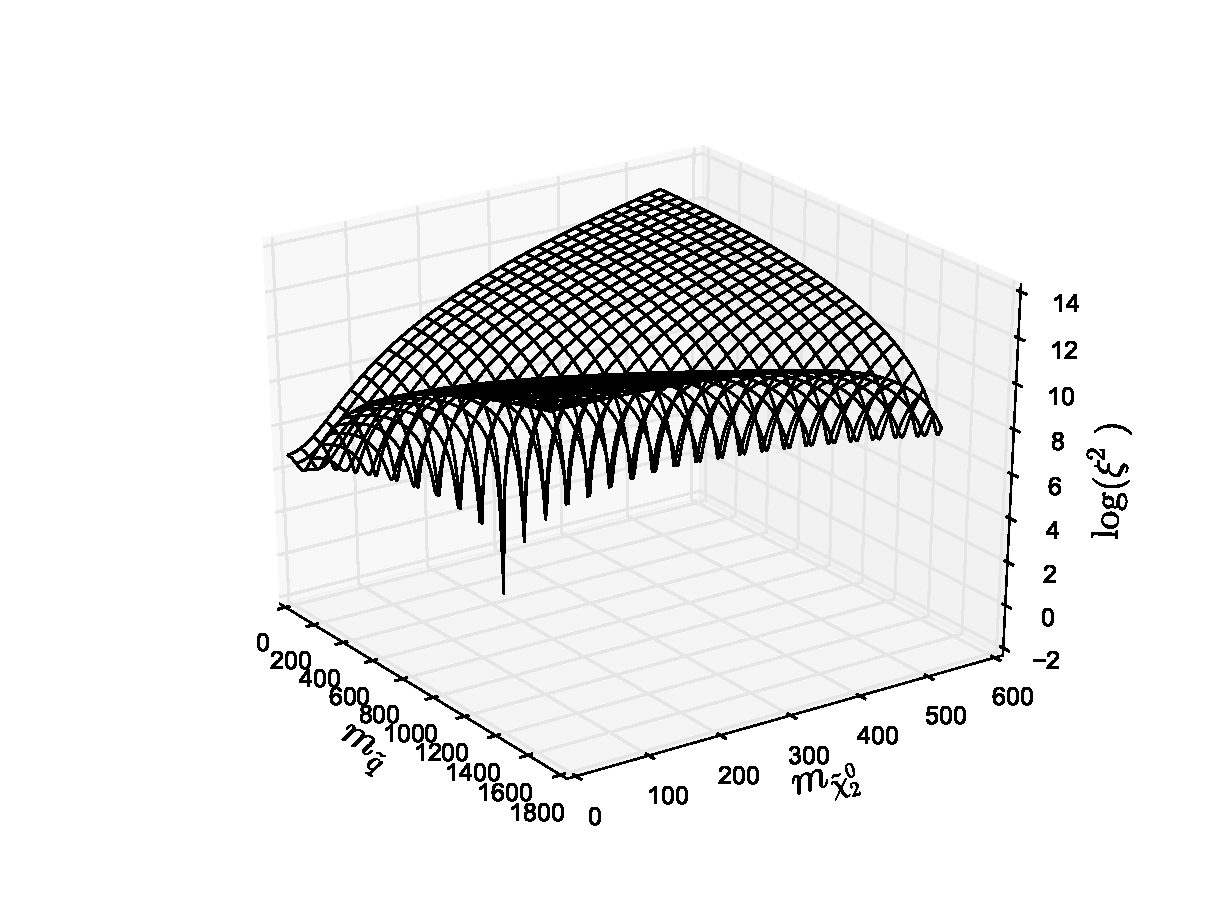
\includegraphics[width=\textwidth]{figures/3D_plot_xisquared_1_simplistic_event_squark-chi2.pdf} 
% 		\caption{}
% 		% \label{fig:3D_masses1}
% 	\end{subfigure}
% 	\begin{subfigure}[b]{0.49\textwidth}
% 		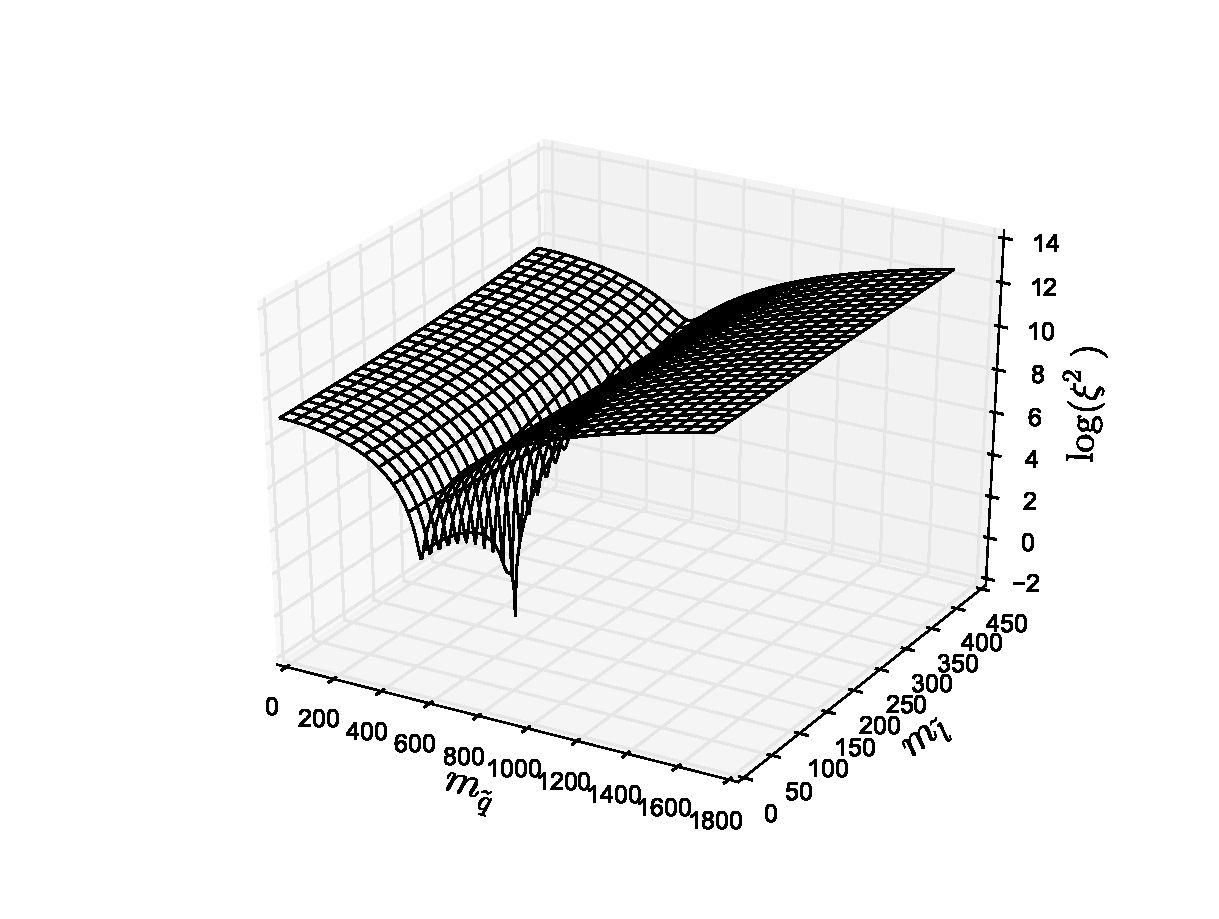
\includegraphics[width=\textwidth]{figures/3D_plot_xisquared_1_simplistic_event_squark-slepton.pdf} 
% 		\caption{}
% 		% \label{fig:3D_masses2}
% 	\end{subfigure}

% 	\begin{subfigure}[b]{0.49\textwidth}
% 		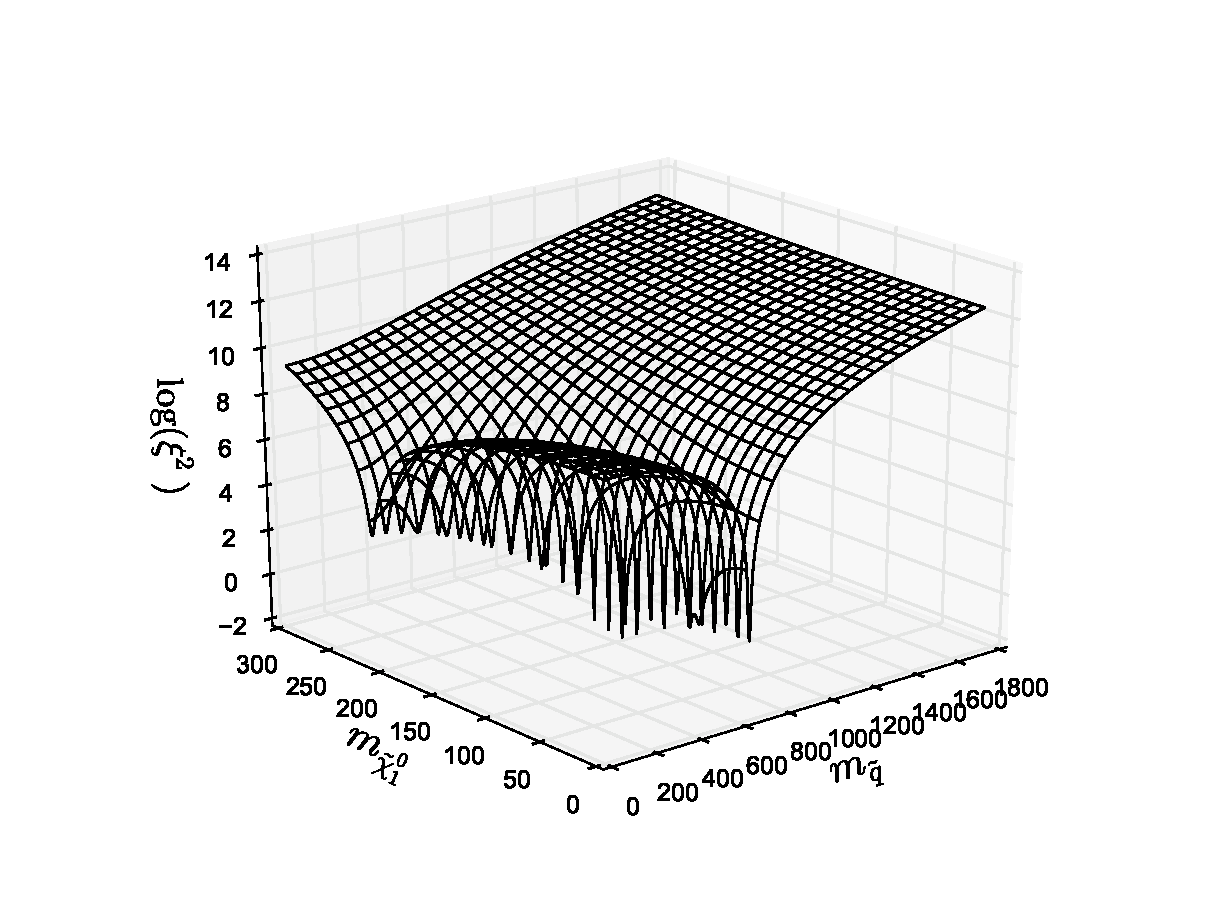
\includegraphics[width=\textwidth]{figures/3D_plot_xisquared_1_simplistic_event_squark-chi1.pdf} 
% 		\caption{}
% 		% \label{fig:3D_masses3}
% 	\end{subfigure}
% 	% \begin{subfigure}[b]{0.49\textwidth}
% 	% 	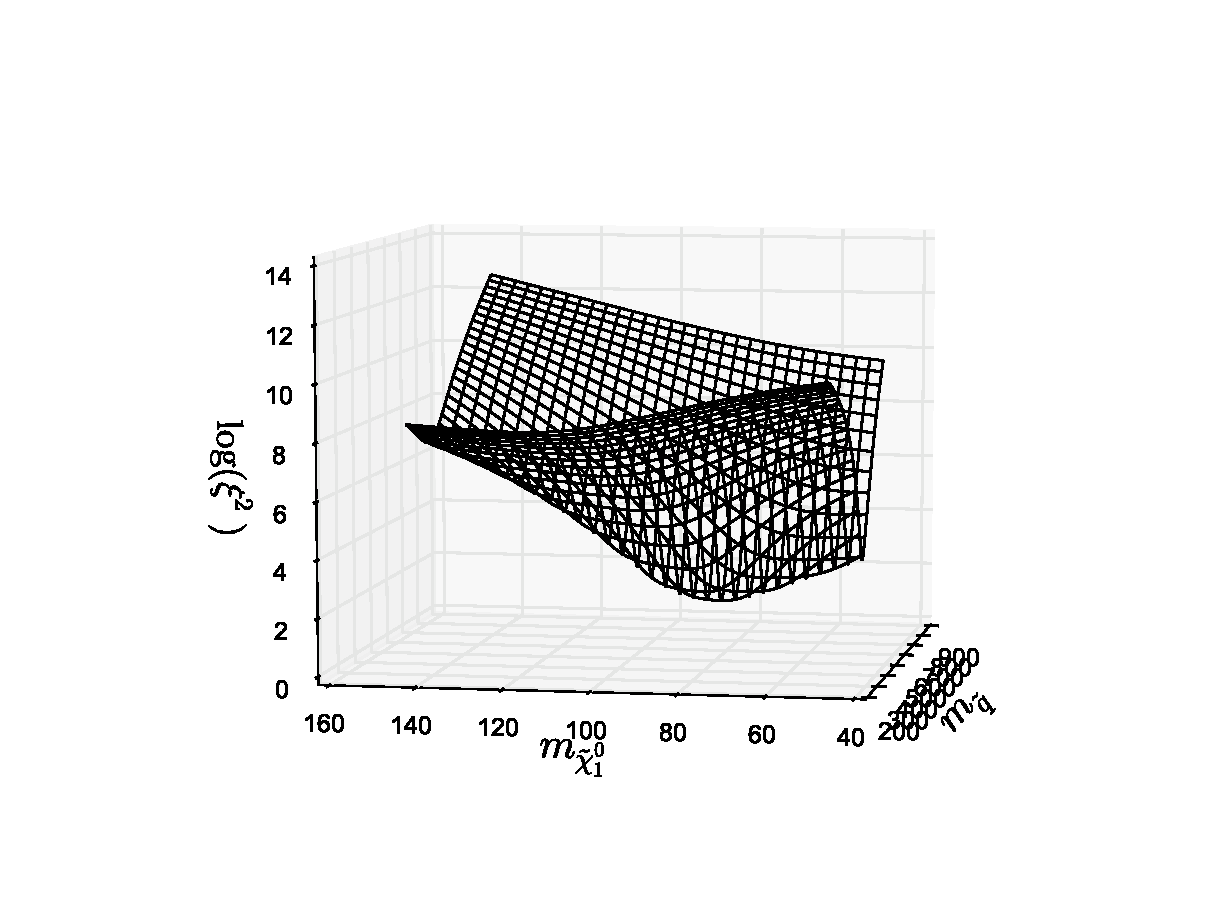
\includegraphics[width=\textwidth]{figures/3D_plot_xisquared_25_herwig_events_squark-chi1_rotated.pdf} 
% 	% 	\caption{}
% 	% 	\label{fig:3D_masses4}
% 	% \end{subfigure}
% 	\caption{3D contour plot of $\log(\xi^2)$ in $m_{\tilde q}-m_i$ plane around the point of true minimum, where $i=\tilde \chi_2^0$ for (a), $i=\tilde l$ for (b) and $i=\tilde \chi_1^0$ for (c) and (d). The other two masses are fixed to their true value. The plot is for a sample of 25 events. Note that the `spikes' are an artifact of the plotting style.}
% 	\label{fig:3D_masses_simplistic_1event}
% \end{figure}

% Using the numerical minimization method Nelder-Mead, or `Simplex method', we find the numerical minimum of the $\xi^2$. This is non-trivial, and the problems of minimization will be thoroughly discussed throughout this thesis. The problem seems mainly to be that numerical minimization routines rely on getting a starting point from the user. When we have generated the events ourselves, we of course know the true value of the masses -- which we expect to be very close to the minimum of the function, if not exactly at the spot -- but in an experimental situation we will have little or no information about where to search. 

% In table \ref{table:starting_point_fit_dependency_1event_simplistic} we present the results of numerical searches for the minimum of the $\xi^2$ shown in \ref{fig:3D_masses_simplistic_1event} for different starting points. The points are chosen as a multiple $x$ of the true mass values. \marginpar{This means we only vary them along a line in 4D. Worth trying other parametrizations.} We see that the fit is highly dependent on starting point. This might be explained by the `valley' shape of the $\xi^2$ seen in the plots -- it is plausible that the minimization algorithm has problems with resolving the true minimum when there are two directions with very different steepness as here.

% \begin{table}[hbt]
% 	\centering
% 	\begin{tabular}{| l | l | l | l | l | l |}
% 		\hline
% 		Starting point  &&&&																					&  Minimal $\xi^2$ \\ 
% 		 						& $\tilde q$	& $\tilde \chi_2^0$	& $\tilde l$	& $\tilde \chi_1^0$ & value \\ \hline
% 		True mass [GeV]			& 568.0         & 180.3 			& 144.1			&  97.0				& \\ \hline
% 		100 \% 					& 568.0  		& 180.3   			& 144.1  		&  97.0				& $7.2\times 10^{-30}$ \\ \hline
% 		90 \% 					& 532.5  		& 164.9   			& 124.7  		&  90.0				& $2.4\times 10^{-28}$ \\ \hline
% 		110 \%					& 620.1  		& 202.2   			& 163.2  		& 107.8				& $6.0\times 10^{-28}$ \\ \hline
% 		50 \% 					& 515.0  		& 135.2   			&  74.1  		&   8.9				& $9.2\times 10^{-30}$ \\ \hline
% 		150 \% 					& 810.1  		& 274.9   			& 229.5  		& 139.5				& $3.3\times 10^{-27}$ \\ \hline
% 	\end{tabular}
% 	\caption{The minimal point found by Scipy Nelder-Mead for a $\xi^2$ from one event of squarks decaying from rest, for different starting points.}
% 	\label{table:starting_point_fit_dependency_1event_simplistic}
% \end{table}

% The strength in Webber's approach, however, lies in the ability to combine multiple events in one fit. We make the same plot again, but with 25 events combined, in figure \ref{fig:3D_masses_simplistic}. We immediately notice that most of the ``valley''-like features of the previous plot have disappeared, the surface is flatter, and the minima are more pronounced. When we now apply the minimization algorithm, we find a much better performance, and the correct best-fit point is found to 1 decimal point in most cases. The results are summarized in table \ref{table:starting_point_fit_dependency_25events_simplistic}. Note that for a starting point of $x = 0.5$, the algorithm finds the unphysical point $-97$ GeV for the LSP mass. This is probably an artifact due to that the $\xi^2$ is symmetric in mass sign, and that the Nelder-Mead algorithm is unable to handle constraints or bounds (so we cannot specify that the masses must be positive).

% \begin{table}[hbt]
% 	\centering
% 	\begin{tabular}{| l | l | l | l | l | l |}
% 		\hline
% 		Starting point  &&&&																					&  Minimal $\xi^2$ \\ 
% 		 						& $\tilde q$	& $\tilde \chi_2^0$	& $\tilde l$	& $\tilde \chi_1^0$ & value \\ \hline
% 		True mass [GeV]			& 568.0         & 180.3 			& 144.1			& 97.0				& \\ \hline
% 		100 \% 					& 568.0   		& 180.3   			& 144.1   		& 97.0      		& 1.482195e-26 \\ \hline
% 		90 \%  					& 568.0   		& 180.3   			& 144.1   		& 97.0      		& 5.842969e-27 \\ \hline
% 		110 \% 					& 568.0   		& 180.3   			& 144.1   		& 97.0      		& 4.779690e-27 \\ \hline
% 		50 \%  					& 568.0   		& 180.3   			& 144.1   		& $-97.0$     		& 6.303178e-27 \\ \hline
% 	\end{tabular}
% 	\caption{The minimal point found by Scipy Nelder-Mead for a $\xi^2$ of 25 events of squarks decaying from rest, for different starting points.}
% 	\label{table:starting_point_fit_dependency_25events_simplistic}
% \end{table}


% \begin{figure}[hbt]
% 	\centering
% 	\begin{subfigure}[b]{0.49\textwidth}
% 		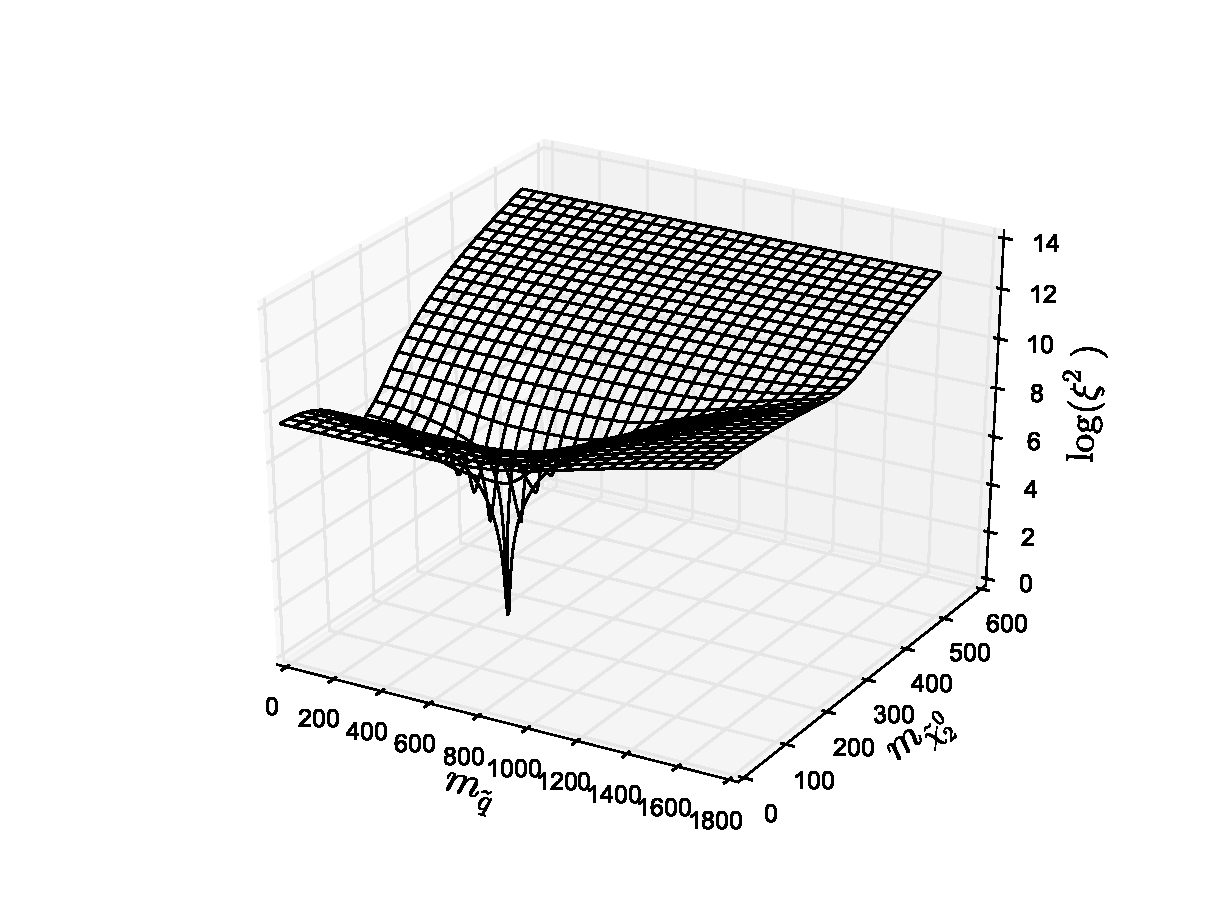
\includegraphics[width=\textwidth]{figures/3D_plot_xisquared_25_simplistic_events_squark-chi2.pdf} 
% 		\caption{}
% 		% \label{fig:3D_masses1}
% 	\end{subfigure}
% 	\begin{subfigure}[b]{0.49\textwidth}
% 		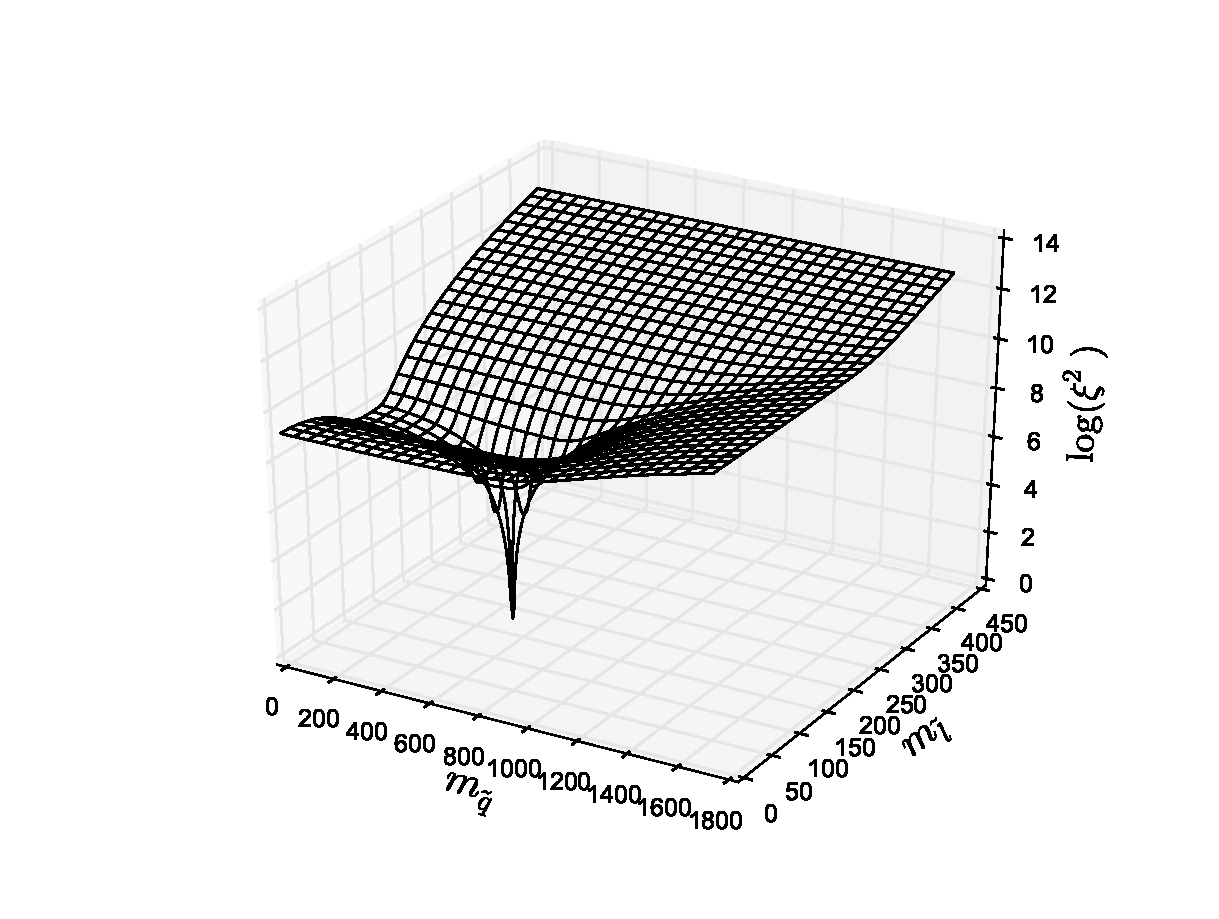
\includegraphics[width=\textwidth]{figures/3D_plot_xisquared_25_simplistic_events_squark-slepton.pdf} 
% 		\caption{}
% 		% \label{fig:3D_masses2}
% 	\end{subfigure}

% 	\begin{subfigure}[b]{0.49\textwidth}
% 		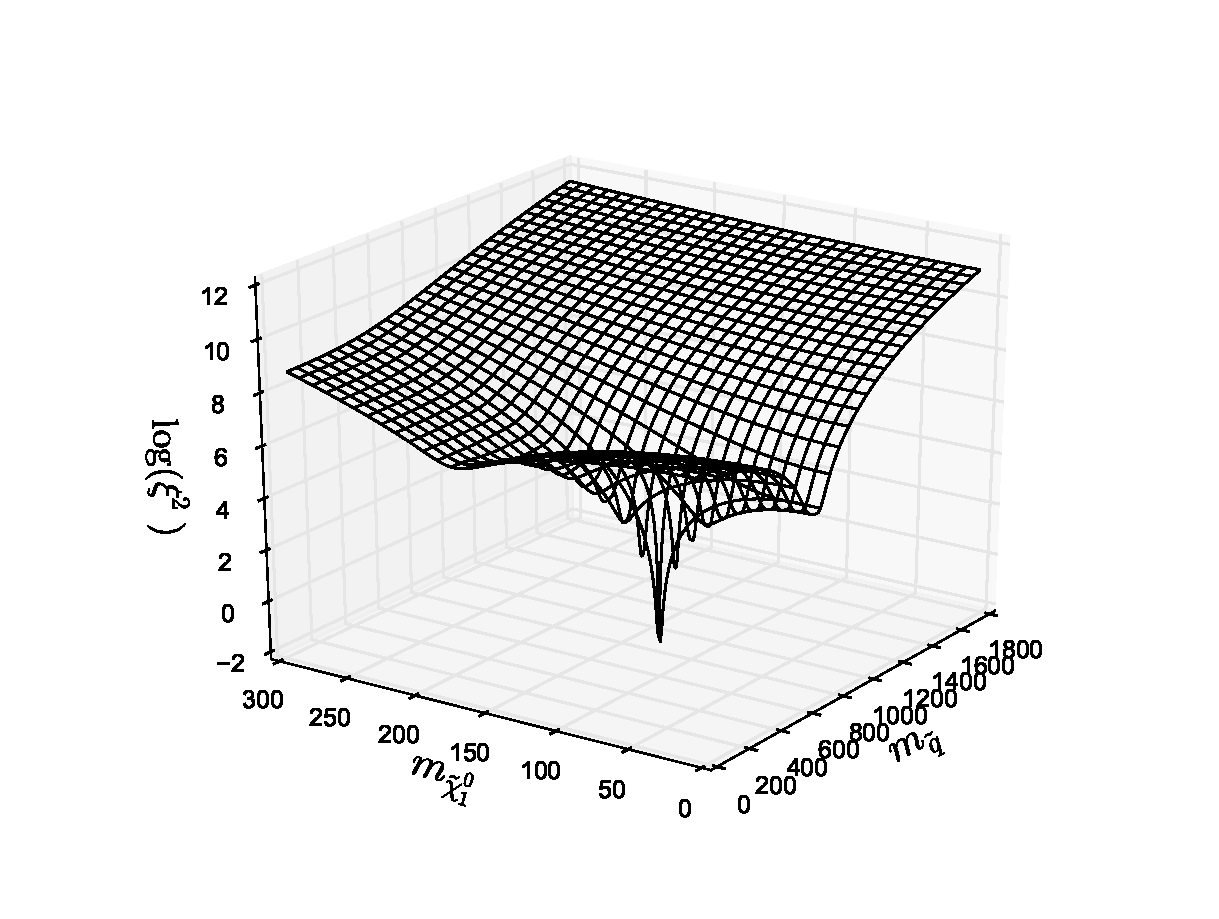
\includegraphics[width=\textwidth]{figures/3D_plot_xisquared_25_simplistic_events_squark-chi1.pdf} 
% 		\caption{}
% 		% \label{fig:3D_masses3}
% 	\end{subfigure}
% 	% \begin{subfigure}[b]{0.49\textwidth}
% 	% 	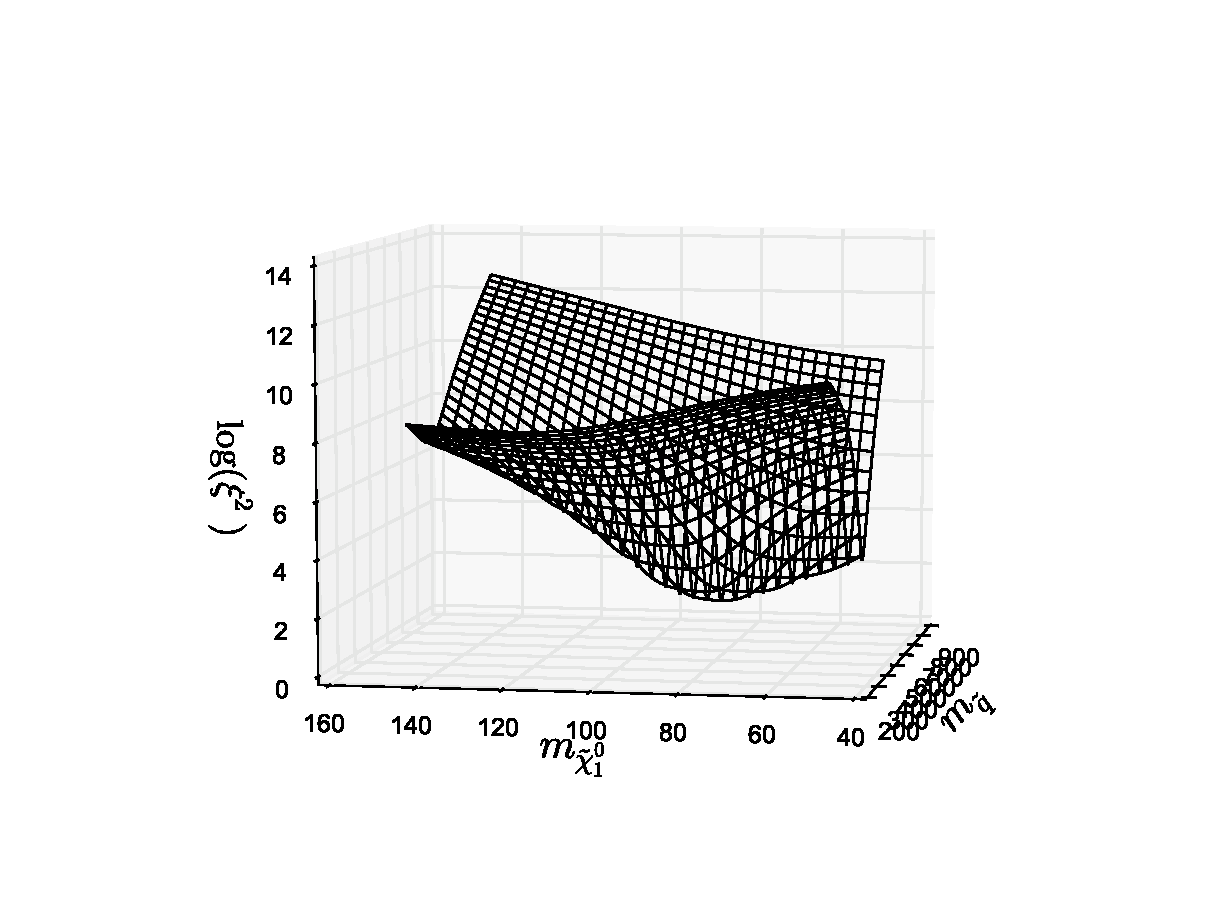
\includegraphics[width=\textwidth]{figures/3D_plot_xisquared_25_herwig_events_squark-chi1_rotated.pdf} 
% 	% 	\caption{}
% 	% 	\label{fig:3D_masses4}
% 	% \end{subfigure}
% 	\caption{3D contour plot of $\log(\xi^2)$ in $m_{\tilde q}-m_i$ plane around the point of true minimum, where $i=\tilde \chi_2^0$ for (a), $i=\tilde l$ for (b) and $i=\tilde \chi_1^0$ for (c) and (d). The other two masses are fixed to their true value. The plot is for a sample of 25 events.}
% 	\label{fig:3D_masses_simplistic}
% \end{figure}

% We now make a fit of 100 bins of 25 events of this simple kind. The results are summarized in table \ref{table:fits_100_bins_simplistic}, and scatter plots of the best-fit points are shown in figure \ref{fig:fits_100_bins_simplistic}. The fits are very good in most cases, except for $x = 50 \%$, where it fails to find the best-fit point in many cases. Also, the scatter plots reveal the tendency of the best-fit points to distribute themselves along lines in the southwest/northeast-direction of the mass planes, intersecting the points of true minimum. This is the same direction that the `valley' shape takes in the surface plots, indicating that the inaccuracy in the minimization is hardest to resolve in the direction of the valley.

% \begin{table}[hbt]
% 	\centering
% 	\begin{tabular}{| l | l | l | l | l | l |}
% 		\hline
% 		Starting point &  $m_{\tilde{q}}$ & $m_{\tilde{\chi}_2^0}$ & $m_{\tilde{l}}$ & $m_{\tilde{\chi}_1^0}$ \\ \hline
% 					   & True values [GeV] 	& 568 (avg.) 	& 180 	& 144 	& 97 \\ \hline
% 		100 \%		   & $568 \pm 0$ & $180 \pm 0 $ & $144 \pm 0 $ & $97 \pm 0	$ \\ \hline
% 		90 \% 		   & $568 \pm 0$ & $180 \pm 0 $ & $144 \pm 0 $ & $97 \pm 0	$ \\ \hline
% 		110 \%		   & $568 \pm 1$ & $180 \pm 1 $ & $144 \pm 1 $ & $97 \pm 1	$ \\ \hline
% 		50 \% 		   & $567 \pm 4$ & $175 \pm 36$ & $142 \pm 10$ & $-20 \pm 92$   \\ \hline
% 		150 \%		   & $568 \pm 2$ & $181 \pm 4 $ & $145 \pm 5 $ & $98 \pm 6 $	 \\ \hline
% 	\end{tabular}
% 	\caption{Fit of 100 bins of 25 simplistic events using SciPy Nelder-Mead. Values are given as average $\pm$ r.m.s. deviation. }
% 	\label{table:fits_100_bins_simplistic}
% \end{table}



% \begin{figure}[hbt]
% 	\centering
% 	\begin{subfigure}[b]{0.49\textwidth}
% 		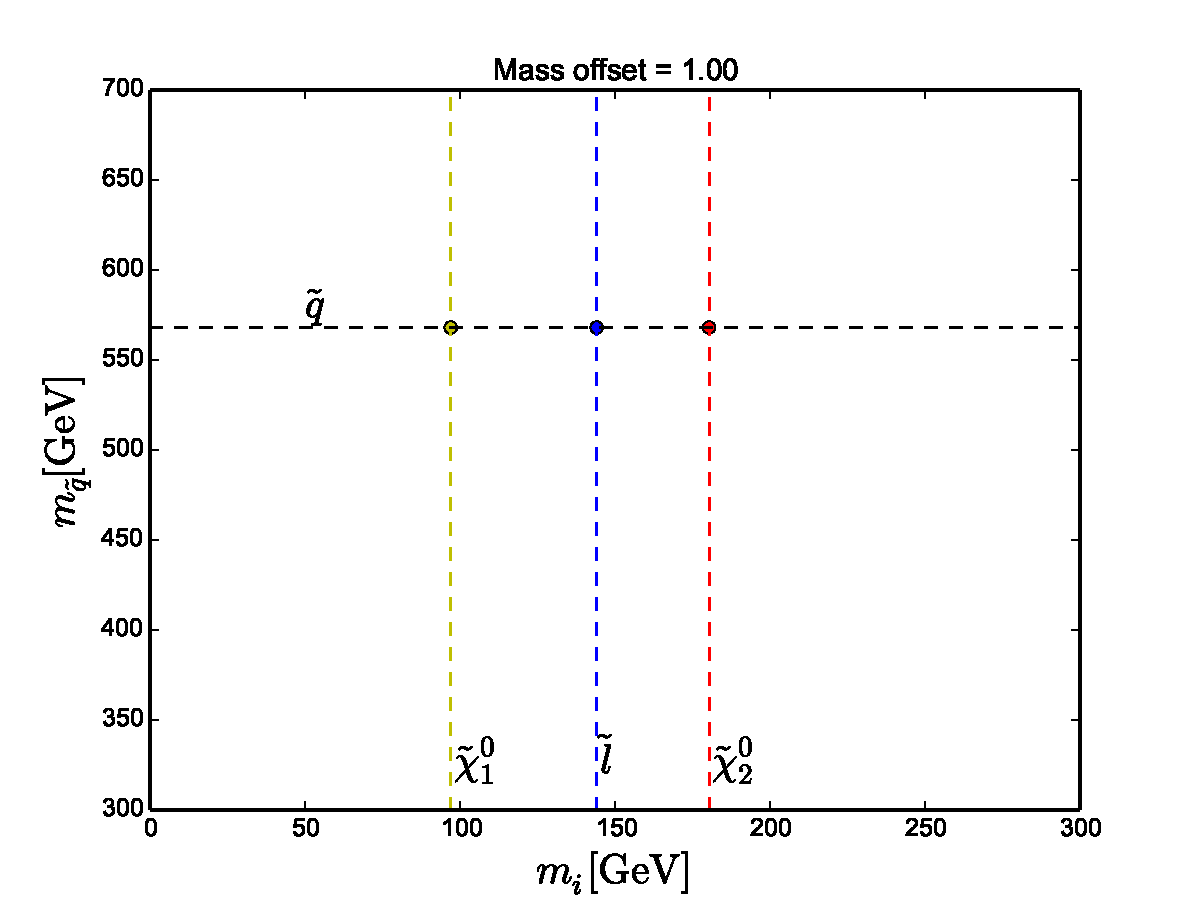
\includegraphics[width=\textwidth]{figures/25_events_simplistic_scipy_nelder-mead_without_smearing_1p00_initial_guess.pdf} 
% 		\caption{}
% 	\end{subfigure}
% 	\begin{subfigure}[b]{0.49\textwidth}
% 		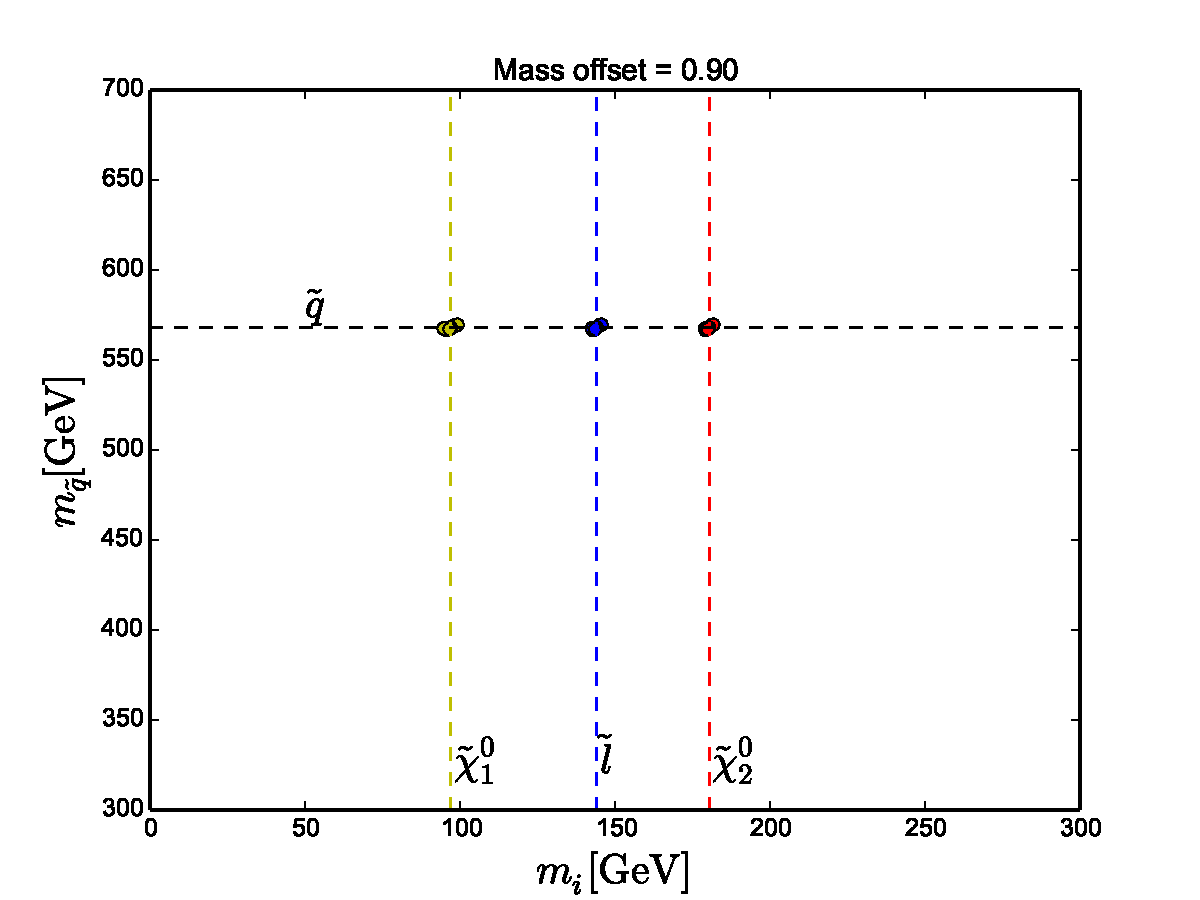
\includegraphics[width=\textwidth]{figures/25_events_simplistic_scipy_nelder-mead_without_smearing_0p90_initial_guess.pdf} 
% 		\caption{}
% 	\end{subfigure}

% 	\begin{subfigure}[b]{0.49\textwidth}
% 		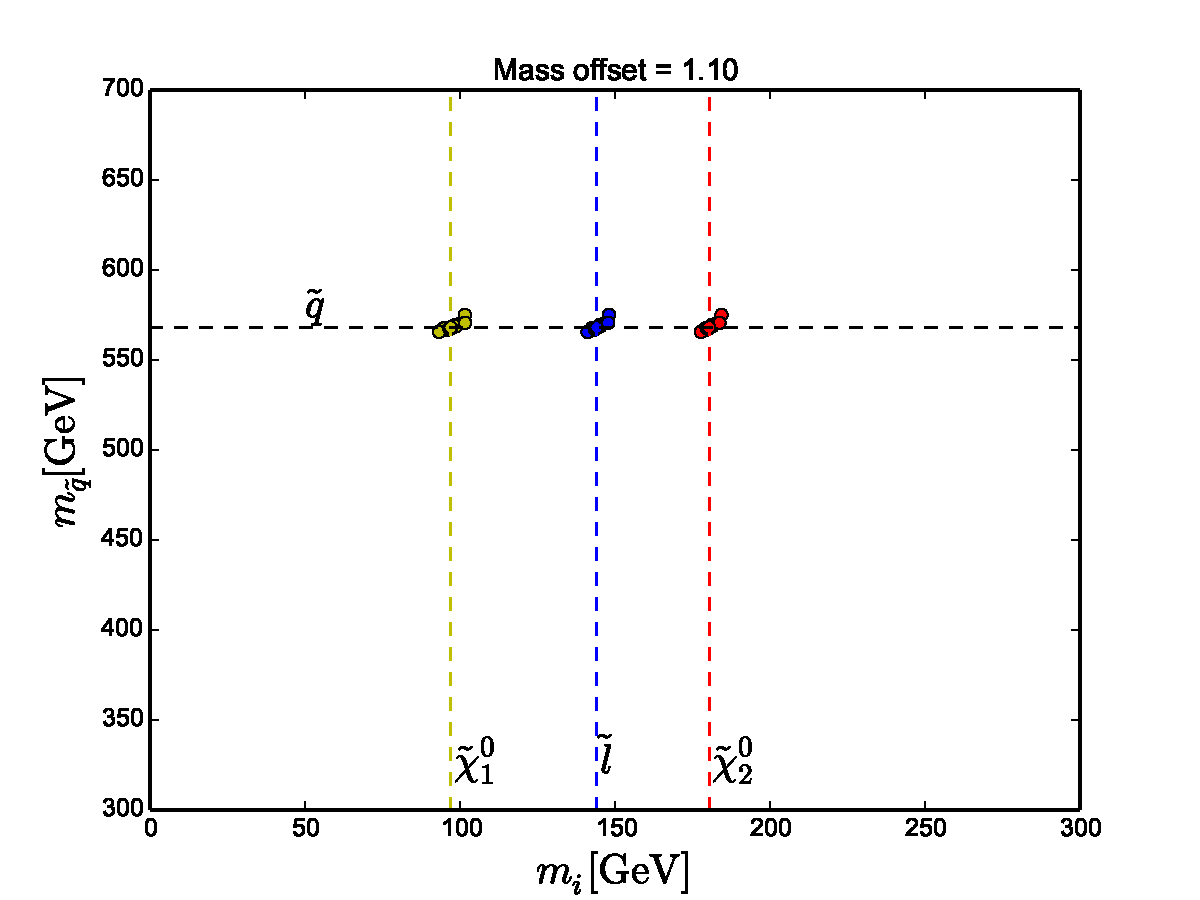
\includegraphics[width=\textwidth]{figures/25_events_simplistic_scipy_nelder-mead_without_smearing_1p10_initial_guess.pdf} 
% 		\caption{}
% 	\end{subfigure}
% 	\begin{subfigure}[b]{0.49\textwidth}
% 		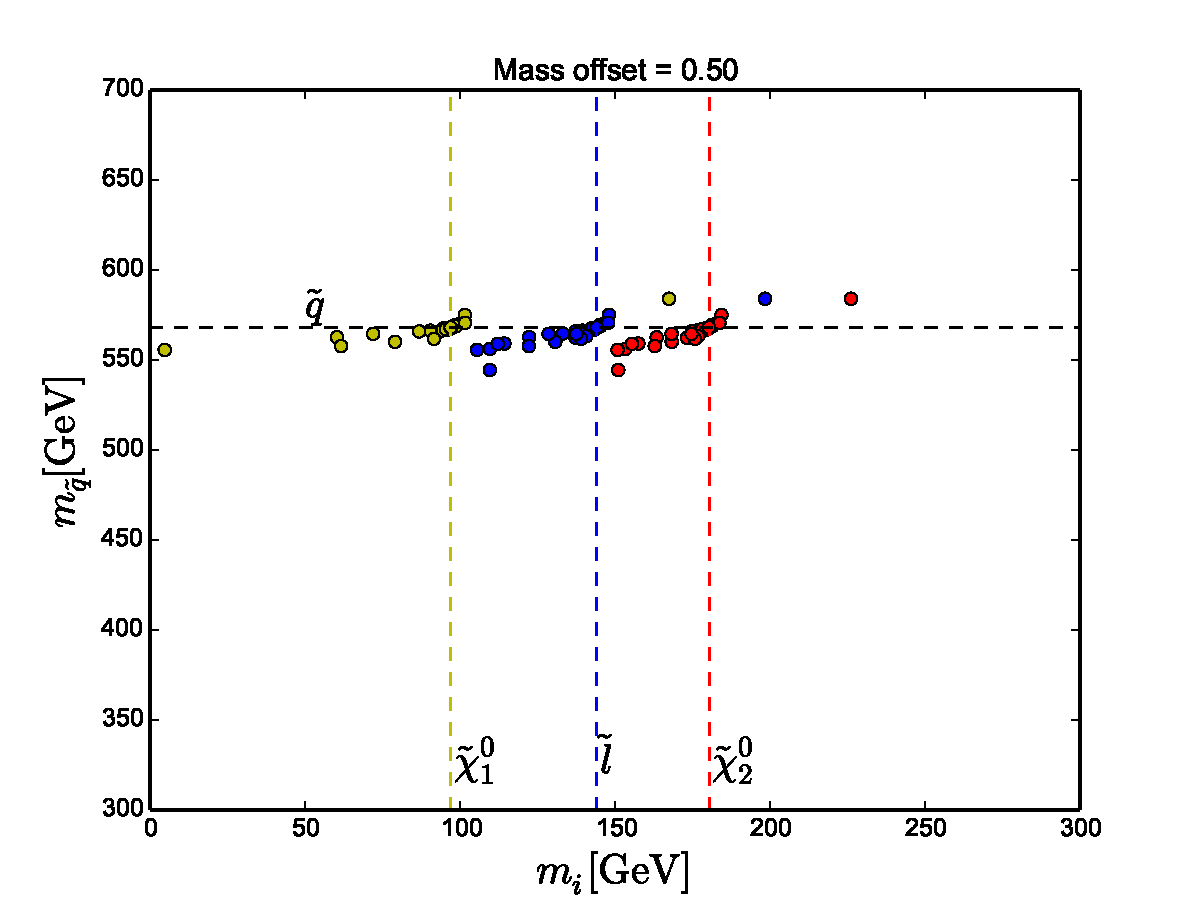
\includegraphics[width=\textwidth]{figures/25_events_simplistic_scipy_nelder-mead_without_smearing_0p50_initial_guess.pdf} 
% 		\caption{}
% 	\end{subfigure}

% 	\begin{subfigure}[b]{0.49\textwidth}
% 		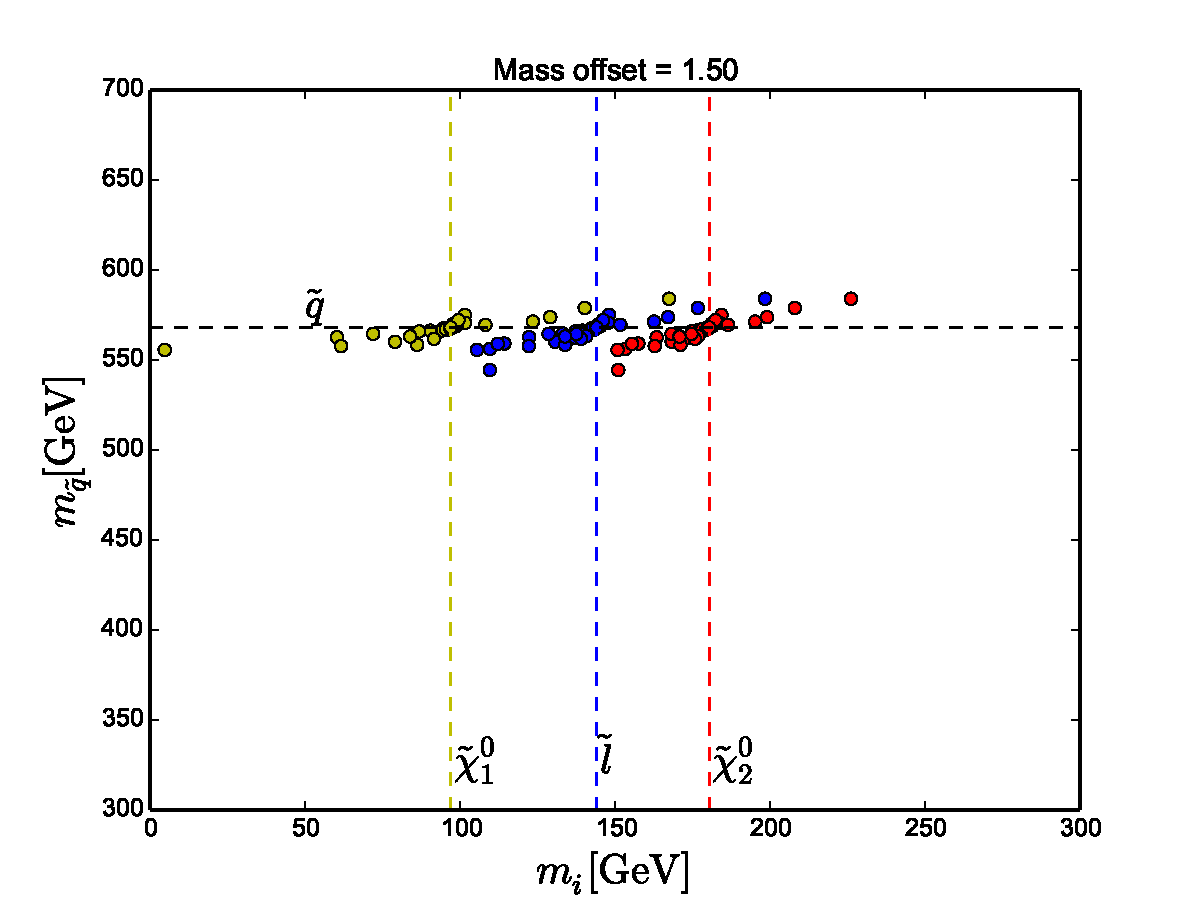
\includegraphics[width=\textwidth]{figures/25_events_simplistic_scipy_nelder-mead_without_smearing_1p50_initial_guess.pdf} 
% 		\caption{}
% 	\end{subfigure}
% 	\caption{Scatter plots of 100 bin fits of 25 simplistic events for different starting points, corresponding to table \ref{table:fits_100_bins_simplistic}.}
% 	\label{fig:fits_100_bins_simplistic}
% \end{figure}



% % \section{Event generation using {\tt CompHEP}}
% % We first begin by using {\ttfamily CompHEP 4.5.2} \cite{Pukhov:1999gg} to generate 1000 $pp \to \tilde{u}_L \bar{\tilde{u}}_L$ collisions at $\sqrt{s} = 14 \, \mathrm{TeV}$ with the supersymmetric parameter choice mSUGRA SPS1a $(\alpha)$ \cite{Allanach:2002nj} calculated using {\ttfamily SoftSUSY 3.4.1} \cite{Allanach:2001kg}.\footnote{Note that CompHEP uses the wrong squark mass: The value from SoftSUSY is $\sim 565 \,\mathrm{GeV}$, while CompHEP uses $\sim 545 \,\mathrm{GeV}$. This is due to how CompHEP is coded: The external RGE running done by SoftSUSY is only used by CompHEP up to the point of low-scale soft mass parameters. The calculation of physical squark masses from soft mass parameters is hard-coded in CompHEP using a tree-level formula. Trying to manually change the value has proven difficult since it disturbs the internal consistency of CompHEP.} \marginpar{TODO: Make CompHEP use the correct squark mass if possible.} {\ttfamily CompHEP} produces a file containing the 4-momenta of the squarks for each event. It is important to note that {\ttfamily CompHEP} produces the squarks on-shell -- possibly a major simplification for colour-charged particles, who might realistically be far off-shell when they come from a hard collision before they have a chance to shower off gluons. The squark 4-momenta are then read into a Python script where the rest of the chain is generated. We generate the chain as a succession of two-body decays where the decay products are on-shell, {\it e.g.}\ we work in a narrow width approximation. This is again a major simplification for the quark due to showering. Standard model particles are assumed massless. The algorithm for this generation is described in section \ref{sec:decayalgorithm}. The decay direction for the back-to-back decay in each step is drawn uniformly on a sphere. This is correct for the scalar particles, and for the fermions it is justified by averaging over spin directions. \marginpar{\color{purple} Note to self: Check that I understand this properly.} The resulting visible 4-momenta resemble an idealized decay situation. As a check to see that our algorithm is correct, we reproduce the dilepton invariant mass distribution for the upper chain as discussed in the previous section. The distribution is shown in figure \ref{fig:dilepton_invariant_mass_no_smearing}. We see that it resembles a triangle, and that it cuts sharply at $m_{ll}^{\mathrm{max}} \approx 80 \, \mathrm{GeV}$, which corresponds nicely with the theoretical prediction $m_{ll}^\text{max} = 80.2 \, \mathrm{GeV}$ from Eq. \ref{eq:invariant_mass_endpoint}.

% % \begin{figure}[hbt]
% % \centering
% % 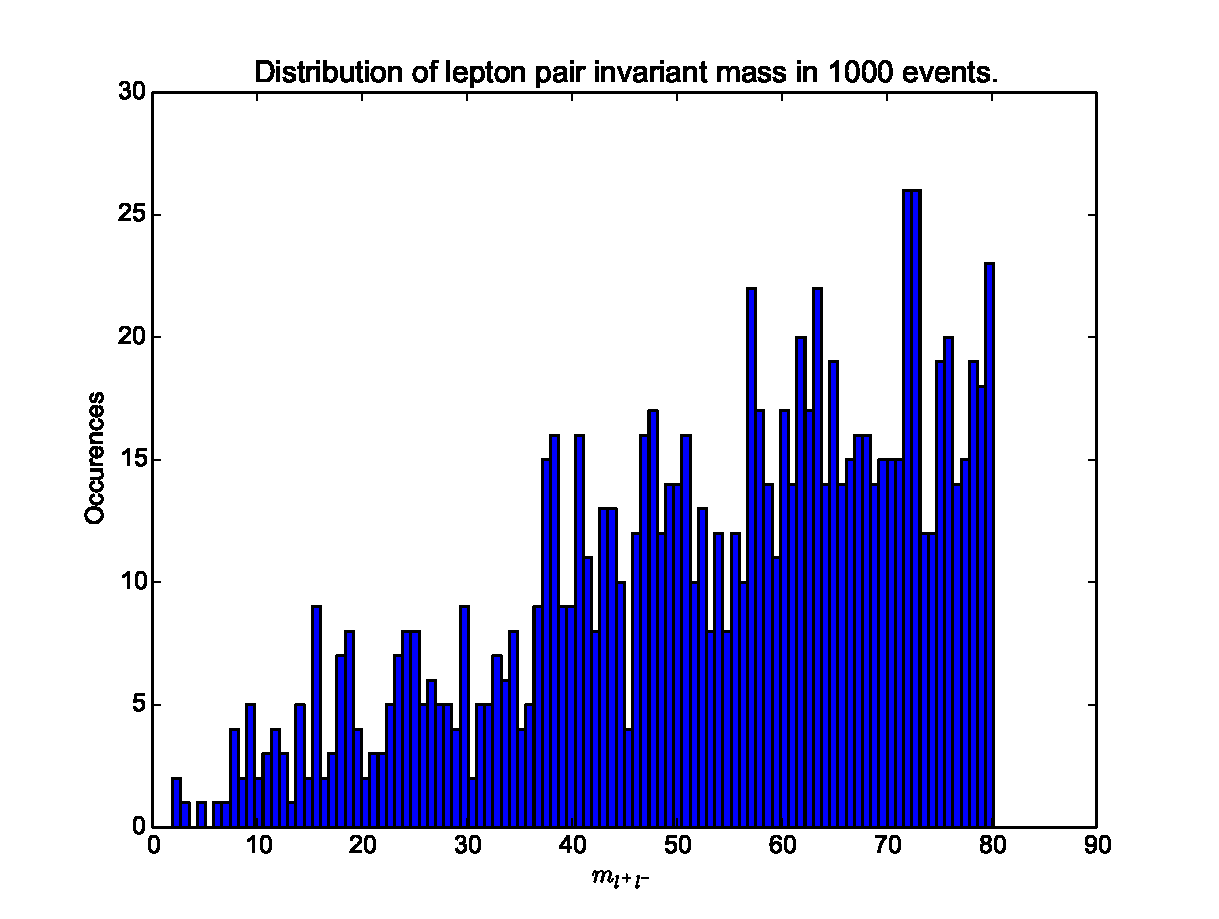
\includegraphics[scale=0.7]{figures/dilepton_invariant_mass_comphep-data_smearing-0_events-1000.pdf} 
% % \caption{Dilepton invariant mass distribution.}
% % \label{fig:dilepton_invariant_mass_no_smearing}
% % \end{figure} \marginpar{Redo dilepton invmass plot with fewer bins and larger font. Also change colour?}



% % \section{$\xi^2$ minimization}
% % \marginpar{This paragraph is up for deletion.}
% % {\color{gray} We also test the mass reconstruction method on this idealized dataset. Webber uses the {\ttfamily MINUIT} algorithm {\ttfamily SIMPLEX}, which we also apply. We use it in the form of the python package {\ttfamily PyMinuit} \cite{PyMinuit,James:1975dr}. Applying {\ttfamily SIMPLEX} to the method, using the entire dataset of 1000 events, gives excellent results -- way too good to be realistic, as we might anticipate, given the high level of idealization and large number of events. Data from fitting 1000 events is shown in table \ref{table:fit_no_smear}. We see that the error in the fit is at the level of a few percent.}
% % \marginpar{Note: The mass used for generation is the comphep-wrong one. Should redo with proper mass if I can fix the problem.}

% % \begin{table}[hbt]
% % 	\centering
% % 	\begin{tabular}{| l | l | l | l | l |}
% % 		\hline
% % 							&  $m_{\tilde{q}}$ & $m_{\tilde{\chi}_2^0}$ & $m_{\tilde{l}}$ & $m_{\tilde{\chi}_1^0}$ \\ \hline
% % 		True values [GeV] 	& 545.4 & 180.3 & 144.1 & 97.0 \\ \hline
% % 		Best-fit values [GeV] & 546.8 & 184.2 & 148.9 & 104.0 \\ \hline
% % 		Relative fit error  & 0.2 \% & 2.1 \% & 3.3 \% & 7.2 \% \\ \hline
% % 	\end{tabular}
% % 	\caption{SIMPLEX fit of 1000 events in an idealized situation.}
% % 	\label{table:fit_no_smear}
% % \end{table}

% % We split the events in 25 event bins and apply the method to each bin. For the minimization we employ {\ttfamily SciPy} \cite{SciPy} with TNC \cite{Nash:1984}. We try several choices for the initial parameter guess, to investigate how different starting points affect minimization performance.

% % \begin{table}[hbt]
% % 	\centering
% % 	\begin{tabular}{| l | l | l | l | l |}
% % 		\hline 
% % 		x $\backslash$ Particle   			& $\tilde q$ 	&$\tilde \chi_2^0$ 	& $\tilde l$ 	& $\tilde \chi_1^0$    	\\ \hline
% % 		True mass [GeV]     & 568 (average) & 180				& 144			& 97					\\
% % 		1.1 &	$570 \pm 15 [29]$ & $196 \pm 5 [17]$ & $159 \pm 4 [15]$ & $111 \pm 6 [16]$ \\
% % 		0.9 &	$526 \pm 16 [25]$ & $166 \pm 5 [15]$ & $130 \pm 3 [15]$ & $80 \pm 6 [18]$ \\
% % 		0.5 &	$445 \pm 75 [123]$ & $118 \pm 24 [67]$ & $84 \pm 17 [62]$ & $28 \pm 20 [72]$ \\
% % 		2.0 &	$824 \pm 184 [334]$ & $334 \pm 37 [159]$ & $285 \pm 24 [143]$ & $221 \pm 34 [129]$ \\ \hline
% % 	\end{tabular}
% % 	\caption{Summary of TNC fits to 25 event bins corresponding to figure \ref{fig:comphep_scipy_TNC_fits}. Fitted parameters are given as `average over bins $\pm$ empirical rms variation [true rms variation]'. The true rms variation means rms deviation from the true mass value rather than the mean. The $x$'s are defined such that $M_\mathrm{initial}= x M_\mathrm{true}$ for all unknown masses, $M_\mathrm{initial}$ being the starting point of the search.}
% % 	\label{table:comphep_scipy_TNC_fits}
% % \end{table}

% % \begin{figure}[hbt]
% % 	\centering
% % 	\begin{subfigure}[b]{0.49\textwidth}
% % 		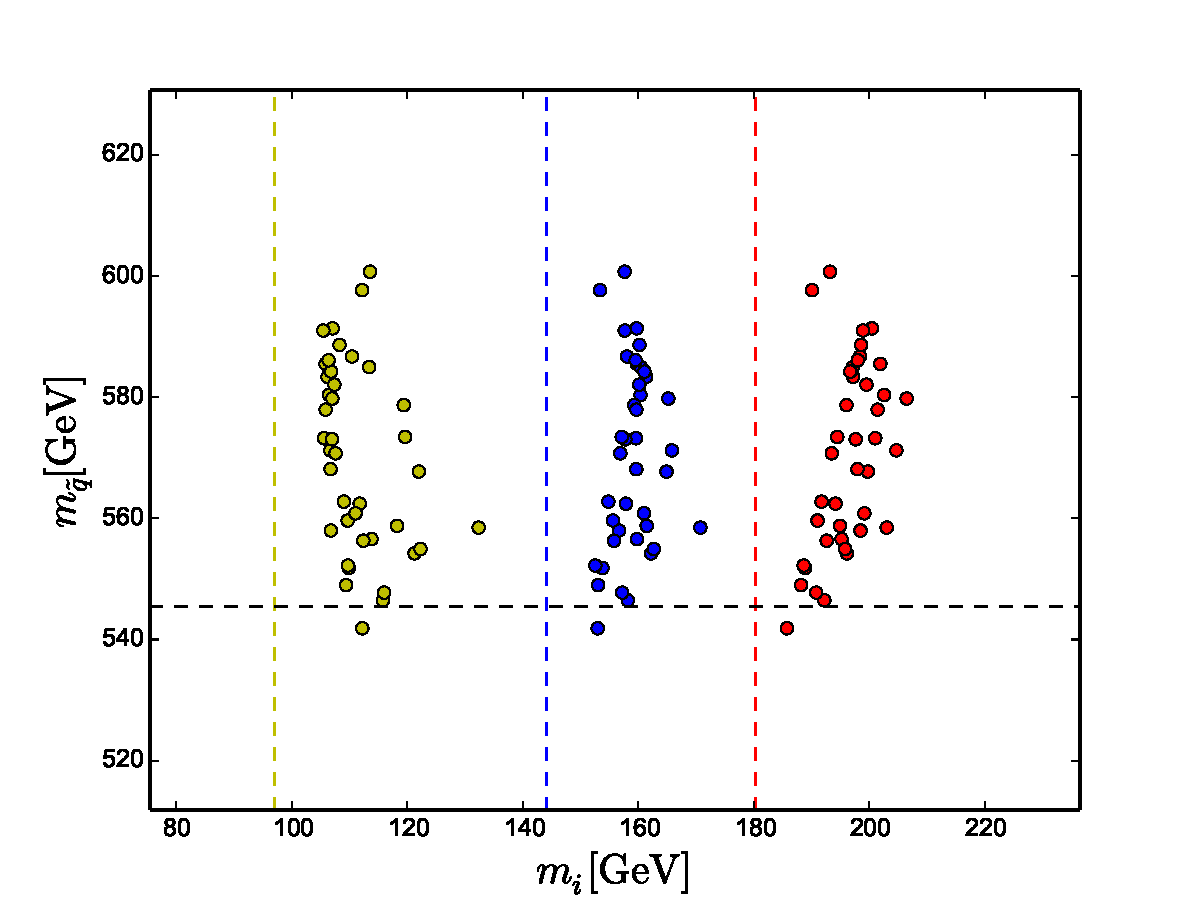
\includegraphics[width=\textwidth]{figures/comphep_scipy_TNC_fit_1p1_initial_guess.pdf} 
% % 		\caption{}
% % 		\label{fig:comphep_scipy_TNC_fits1}
% % 	\end{subfigure}
% % 	\begin{subfigure}[b]{0.49\textwidth}
% % 		\includegraphics[width=\textwidth]{figures/comphep_scipy_TNC_fit_0p9_initial_guess.pdf} 
% % 		\caption{}
% % 		\label{fig:comphep_scipy_TNC_fits2}
% % 	\end{subfigure}

% % 	\begin{subfigure}[b]{0.49\textwidth}
% % 		\includegraphics[width=\textwidth]{figures/comphep_scipy_TNC_fit_2p0_initial_guess.pdf} 
% % 		\caption{}
% % 		\label{fig:comphep_scipy_TNC_fits3}
% % 	\end{subfigure}
% % 	\begin{subfigure}[b]{0.49\textwidth}
% % 		\includegraphics[width=\textwidth]{figures/comphep_scipy_TNC_fit_0p5_initial_guess.pdf} 
% % 		\caption{}
% % 		\label{fig:comphep_scipy_TNC_fits4}
% % 	\end{subfigure}
% % 	\caption{Best-fit points for 40 bins of 25 CompHEP generated events minimized with TNC, with different initial parameter guesses $M_\mathrm{initial} = x M_\mathrm{true}$, where $x = 1.1$ for (a), 0.9 for (b), 2.0 for (c) and 0.5 for (d). The points are summarized in table \ref{table:comphep_scipy_TNC_fits}.}
% % 	\label{fig:comphep_scipy_TNC_fits}
% % \end{figure} 




% % \section{The effects of sorting out dimensions}\marginpar{Note: Consider dropping this section entirely? Or at least redo it with binning, with correct datasets, etc.}
% % It is interesting to see whether our modifications of Webber's mathematics, discussed in section \ref{sec:dimension_fixing}, have any effect on computation time, accuracy or even whether {\ttfamily SIMPLEX} finds the minimum at all. We did a test of this, using 25 of the {\ttfamily CompHEP} events and running through the different smearings $s= 0,0.5,1,3,6$ and $10$. For the basic formulation without the dimension fixing and without normalizing, the {\ttfamily SIMPLEX} routine fails to find the minimum even for zero smearing. Normalizing the $\xi^2$ function by the number of events helps to make it past zero smearing and 0.5 smearing, but then it fails. For zero smearing the mean absolute relative fit error compared to the true masses is at the order of $10^{-7}$. Running with the dimensions of $\mathbf{A}$ fixed according to Eq. \eqref{eq:Amatrix_modified} also fails beyond 0.5 smearing, and the error even for 0 smearing is actually increased to the order of $10^{-2}$. By also including the normalization as given in Eqs. \eqref{eq:vectors_normalized}, the script runs through all smearings and manages to get a fit in every case. We note that the error in this fully dimensionless implementation is of the order $10^{-2}$ for 0 smearing, thus actually higher than for the original implementation. This is however only for one 25 event sample, and should be studied more carefully before drawing conclusions. The total run time for the dimensionless fit is a couple of seconds. By mistake we discovered that dividing the $\xi^2$ by a number of order $10^8$ actually decreased computation time further, by about a factor 2. This indicates that {\ttfamily SIMPLEX} prefers to work with small numbers, at least in the {\ttfamily PyMinuit} implementation.


% \newpage

% \section{Monte Carlo event generation with {\ttfamily Herwig++}}
% % In our fit thus far, we have used events generated by {\ttfamily CompHEP} at squark level and decayed them in a very basic way. One obvious flaw in our model is the lack of {\it parton showering}---the radiation of gluons (and in turn quarks and antiquarks) emitted from the quark in the squark to quark decay process. If showering is taken into account, it means that the initial quark in the squark two-body decay can be off-shell, since it is really carrying the energy and momentum of not only itself, but also (several) other partons.\footnote{This statement should not be taken too literally, since the showering of a discrete number of gluons is just an approximate model of the re-summed contribution from higher-order diagrams in perturbation theory.}

% We employ {\ttfamily Herwig++  2.7.1}~\cite{Bahr:2008pv} for Monte Carlo event generation. This is a complete simulation code for particle collisions, generating hard parton processes from parton distribution functions, handling decays, including (s)particle widths and mass smearing according to Breit-Wigner distributions, initial and final state radiation including parton showering, multiple interactions {\it etc}.\ The user has access to all the information from each event though a {\ttfamily C++} analysis function that can be linked as a library and run by {\ttfamily Herwig++} for each event.

% \subsection{{\ttfamily Herwig++} setup}

% We simulate $pp$ collisions at $\sqrt{s}=14 \, \mathrm{TeV}$. For the following, we turn off the hadronization module in {\ttfamily Herwig++}---treating quarks and gluons as final state particles. 
% %We have to enter a list of the partons that we wish to be able to collide -- we choose $u,d,c,s$ and $g$ plus their antiparticles. 
% We generate sparticle pair production, with the first two generations of left-handed squarks: $\tilde{u}_L,\tilde{d}_L,\tilde{c}_L$ and $\tilde{s}_L$ plus their antiparticles. The exclusion of third-generation squarks from the analysis is done because the difference in masses prevents a good fit under the assumption of a single squark mass. At SPS1a, there is mass degeneracy between left-handed squarks of up- and down-type respectively, for the first two generations. Also, the masses are $m_{\tilde u_L, \tilde c_L} = 565 \,\mathrm{GeV}$ and $m_{\tilde d_L, \tilde s_L} = 571 \, \mathrm{GeV}$, {\it i.e.}\ the up/down-type mass splitting $\Delta m = 6 \, \mathrm{GeV}$ is small. 

% We use only left-handed squarks because the production of $\tilde \chi_2^0$ from right handed squarks is small---at SPS1a the 2nd generation neutralino is mostly wino whilst the 1st generation is mostly bino, and the wino only couples to left-handed squarks. For instance, the branching ratio for $\tilde u_R \to u \tilde \chi_2^0$ is $\sim 1 \%$, whilst for $\tilde u_L$ it is $\sim 30 \%$. The exclusion of events with unwanted squarks is done in the post-generation analysis.

% Furthermore, the mass hierarchy of SPS1a is such that the left-handed sleptons $\tilde e_L, \tilde \mu_L$ are heavier than $\chi_2^0$, thus disabling those decay modes for the $\chi_2^0$. Since first- and second generation sleptons of the same chirality are mass-degenerate at this parameter point, it means that we only have one slepton mass to fit.

% The choice of MSSM parameters is input into {\ttfamily Herwig++} using an SLHA model file~\cite{Skands:2003cj} for the SPS1a parameter point
% generated by {\ttfamily SoftSusy 3.4.1}~\cite{Allanach:2001kg} and post-processed by {\ttfamily SUSY-HIT 1.4} \cite{Djouadi:2006bz} to calculate branching ratios. We disable all decay channels except those that produce our chain (\ref{eq:goldencascade}) by manually editing the branchings in the SLHA file. 

% \subsection{{\ttfamily Herwig++} event analysis routine} 

% A few technical aspects of the per-event analysis done with {\ttfamily Herwig++} should be mentioned. Even though we have disabled all but the relevant decay modes in the simulation, {\ttfamily Herwig++} resets some of the other branchings to small, nonzero values. This means that we must check each event to see that it really contains two instances of the correct cascade. This is done in an analysis routine linked by the {\ttfamily Herwig++} run. At each decay vertex we check that the PDG codes of the outgoing particles match what we expect.

% {\ttfamily Herwig++} showers the squarks and quarks. For the purpose of internal bookkeeping, in the showering process, the event listing will contain several instances of the same particle, {\it e.g.}\ the quark, where the subsequent instances are in a mother-daughter relationship among the event particles. Care has to be taken to ensure that we pick the correct instance of the quark, and we have done tests of momentum conservation to check that we indeed pick the right instance.

% There is also the possibility of photon bremsstrahlung in the other charged particle decays, {\it i.e.}\ the $\tilde \chi_2^0$ and $\tilde l$. This is treated as an $N$-body decay in {\ttfamily Herwig++}, with two massive decay products and $N-2$ photons. We allow these events past our vetoes, and discard the photons -- thus introducing an inaccuracy in the momentum conservation -- on the basis that they would be difficult to identify in a detector event. Since this will only remove energy from the budget, we expect it to potentially lead to some bias toward lower mass values. \marginpar{Note: Here we have the option in the code to veto events with large photon momenta. Should we pursue it?}


% % \subsection{Parton showering}
% % The distribution of quark invariant masses prior to their showering off gluons are shown in figure \ref{fig:invmass_offshellquarks}.

% % \begin{figure}[hbt]
% % \centering
% % \includegraphics[scale=0.7]{figures/quark_invmass_before_showering_both_chains_combined_N1000.pdf} 
% % \caption{Invariant mass distribution of offshell quarks from squark decays. Quarks from both chains in 1000 {\ttfamily Herwig++} generated events are shown. Quark flavours are $u,d,c$ and $s$.}
% % \label{fig:invmass_offshellquarks}
% % \end{figure}

% \section{Fitting the {\ttfamily Herwig++} events}
% The best-fit point is the point which minimizes the $\xi^2$ function, given in Eq. \eqref{eq:xisquared_modified}, for a selection of events. Evaluation of the function involves inverting the $8\times 8$ matrix $\mathbf{A}$ (Eq. \eqref{eq:Amatrix_modified}) for each event, so it is not trivially done by hand, although it is quick to do numerically. But in order to study the behaviour of the $\xi^2$ more in-depth, we implement the method in Mathematica \cite{Mathematica}, which is able to calculate symbolically. Using a sample of 25 events, Mathematica reveals that the $\xi^2$ is a polynomial of degree 8 in the four mass variables. 

% Without taking combinatorical ambiguities into account, the $\xi^2$ function has a smooth surface and a well-defined global minimum\marginpar{Although sometimes it seems like the function is flat around the minimum, or something, since the routines have trouble finding the exact minimum.} -- although it may have several local minima. Figure \ref{fig:3D_masses_herwig} shows the $\log(\xi^2)$ surface as a function of pairs of masses. Notice that the minimum is significantly less pronounced for $m_{\chi_2^0}$ than for the other three masses -- it actually seems to form a slide down toward zero mass. Subfigure (d) shows a rotated view to illustrate this. The plotting limits for each mass is from $0.5$ to $1.5$ of the minimum, so it means that the steepness of $\xi^2$ relative to the lightest mass is less than the others. This may mean that it is more difficult to fit this mass than the others.
% % , which is consistent with our earlier speculations and with the rms errors in table \ref{table:herwig_migrad_nosmear_1p01} -- more on that in a moment. It will be interesting to see how combinatorics affects this. \marginpar{Note to self: Or could this be the result of Migrad not finding a better guess than the initial value for the OTHER masses in many of the bins?}





% \begin{figure}[hbt]
% 	\centering
% 	\begin{subfigure}[b]{0.49\textwidth}
% 		\includegraphics[width=\textwidth]{figures/3D_plot_xisquared_25_herwig_events_squark-chi2.pdf} 
% 		\caption{}
% 		\label{fig:3D_masses1}
% 	\end{subfigure}
% 	\begin{subfigure}[b]{0.49\textwidth}
% 		\includegraphics[width=\textwidth]{figures/3D_plot_xisquared_25_herwig_events_squark-slepton.pdf} 
% 		\caption{}
% 		\label{fig:3D_masses2}
% 	\end{subfigure}

% 	\begin{subfigure}[b]{0.49\textwidth}
% 		\includegraphics[width=\textwidth]{figures/3D_plot_xisquared_25_herwig_events_squark-chi1.pdf} 
% 		\caption{}
% 		\label{fig:3D_masses3}
% 	\end{subfigure}
% 	\begin{subfigure}[b]{0.49\textwidth}
% 		\includegraphics[width=\textwidth]{figures/3D_plot_xisquared_25_herwig_events_squark-chi1_rotated.pdf} 
% 		\caption{}
% 		\label{fig:3D_masses4}
% 	\end{subfigure}
% 	\caption{3D contour plot of $\log(\xi^2)$ in $m_{\tilde q}-m_i$ plane around the point of true minimum, where $i=\tilde \chi_2^0$ for (a), $i=\tilde l$ for (b) and $i=\tilde \chi_1^0$ for (c) and (d). The other two masses are fixed to their true value. The plot is for a sample of 25 events.}
% 	\label{fig:3D_masses_herwig}
% \end{figure}

% To test the fit method, we split the {\ttfamily Herwig++} data into bins of 25 events each. This is the same approach that Webber takes. We use Mathematica's {\ttfamily Minimize} function to find the mass parameter values that minimize the $\xi^2$ for each bin. We study the minimization performance for each bin by making scatter plots and quantize the overall error by looking at the mean value and standard deviation over all the bins.

% Our function seems to have multiple local minima\marginpar{Here I have done a lot of back-and-forth. I think I am landing on that the fitting difficulties seem to be a numerical issue and not due to local minima, although the function in some cases appear to have two or three minima. Also, it turns out that Mathematica's Minimize does NOT in fact do symbolic minimization, but automatically calls a numerical minimizer which uses none other than the Nelder-Mead/Simplex algorithm for minimization. So here I have gone a full round back to start. This sectio was last revised before I did the stuff with on-shell decays from the last section.}, which severely complicates minimization. Most numerical minimization algorithms, such as the Simplex algorithm that Webber uses, relies on getting a starting point from the user. For a function with several minima, a poorly chosen starting point might fool the algorithm to converge to a local minimum without discovering the global minimum. The Mathematica minimization has the advantage of symbolic calculation, so it should have no problem finding the true minimum for a function as simple (sic!) as an octic polynomial in four variables. Also, it does not require a user-supplied starting point, which is nice since we realistically have little idea \`{a} priori of what the mass values are.

% We include an example to illustrate how toublesome the minimization is for the purely numerical routines that Python offer. We use the Truncated Newton's Conjugate Gradient (TNC) method from the Scipy \cite{SciPy} package to minimize three bins of 25 events of unsmeared {\ttfamily Herwig++} data. We choose three different starting points for the minimization, selected as 95 \%, 100 \% and 105 \% of the true mass values, respectively. We limit the parameter space by experimental mass bounds from below. The results are summarized in table \ref{table:starting_point_fit_dependency}. We see that the Scipy minimization depends to a large degree on the starting point. This we have found to be the case for all the numerical methods that are implemented in Scipy, such as Simplex/Nelder-Mead and BFGS. We also see that the Mathematica minimization in all cases performs better or equal to the Scipy method. This gives us confidence that the results obtained by Mathematica reflect the true minima. 

% The explanation for the variable performance of Scipy we believe lies in that the function has local minima somewhere near the true one, at least for some of the events/bins -- it is hard to believe that it cannot handle minimizing a polynomial.\marginpar{But where are they in the plots? Are the plots tricking us since they show only two variables at a time??? Or maybe just the wrong bin is plotted.} It turns out that it is rather tricky to find all local minima of a four-variate function. The local minima are straight-forward to characterize, they are points where all partial derivatives of the function is zero and the Hesse matrix is positive-definite. But to actually find them all has proven to be numerically extensive, to the degree that it brought Mathematica to its knees. (Finding the local minima was the original motivation for employing Mathematica.) This also prompts the question of which starting point Webber uses in his analysis -- he does not mention the problem at all, even though he states that he uses Simplex.\marginpar{This haunts me a bit -- is it possible that Webber uses Simplex in some smart way (e.g. very high tolerance, although I have tried such things) so that it is insensitive to starting point? Since Mathematica has no problems, and it after all only is a polynomial we're minimizing, it seems strange that no numerical method I have tried can manage.}

% % The bins used are the second, third and fourth 25-event bins of the Herwig data. The first Herwig bin fits badly, thus it is not used for this.
% \begin{table}[hbt]
% 	\centering
% 	\begin{tabular}{| l | l | l | l | l | l |}
% 		\hline
% 		Starting point / &&&&																					&  Minimal $\xi^2$ \\ 
% 		Bin number 						& $\tilde q$	& $\tilde \chi_2^0$	& $\tilde l$	& $\tilde \chi_1^0$ & value \\ \hline
% 		True mass [GeV]					& 568 (average) & 180 				& 144 			& 97 				& \\ \hline
% 		95 \%  / 1 						& 628.9   		& 200.0   			& 129.0   		& 46.0     			& 3.095839 \\ \hline
% 		105 \% / 1 						& 634.0   		& 215.8   			& 152.2   		& 92.9     			& 3.108896 \\ \hline
% 		100 \% / 1 						& 633.5   		& 214.0   			& 149.7   		& 88.8     			& 3.107357 \\ \hline
% 		Mathematica / 1 			    & 628.8 		& 200.0				& 128.964,		& 46.				& 3.09584		\\ \hline
% 		95 \%  / 2 						& 445.5   		& 155.3   			& 137.6   		& 112.8    			& 0.1093763 \\ \hline
% 		100 \% / 2 						& 455.1   		& 165.7   			& 146.4   		& 120.9    			& 0.1159998 \\ \hline
% 		105 \% / 2 						& 461.1   		& 170.1   			& 150.2   		& 124.9    			& 0.1214193 \\ \hline
% 		Mathematica / 2 				& 434.1 		& 118.5 			& 94. 			& 51.3 				& 0.104346	\\ \hline
% 		95 \%  / 3 						& 553.2   		& 173.0   			& 133.4   		& 83.5     			& 0.3065114 \\ \hline
% 		100 \% / 3 						& 560.0   		& 179.4   			& 141.2   		& 93.8     			& 0.3074833 \\ \hline
% 		105 \% / 3 				 		& 596.5   		& 192.5   			& 150.7   		& 97.4     			& 0.3432126 \\ \hline
% 		Mathematica / 3 				& 549.3 		& 157.8 			& 113.7 		& 46. 				& 0.303138 \\ \hline	
% 	\end{tabular}
% 	\caption{Example of minimization performance for three different bins of 25 unsmeared {\ttfamily Herwig++} events, minimized using Scipy TNC with three different starting values plus Mathematica. See the text for details.}
% 	\label{table:starting_point_fit_dependency}
% \end{table}

% \newpage % to allow all the \marginpar's to appear! Remove before finalizing.
% \marginpar{Speaking of these bins where the best-fit is outside the allowed region -- should we consider throwing them out? Or maybe throwing 25 events is a little harsh - maybe we can do something on a per-event basis. Anyways, this is more of a discussion for later, when we have smeared and combinatoricized the data so they at least to some small degree resemble reality.} 

% Even though the mathematica routine is clever, it is still a good idea to limit the parameter space as much as possible. Also, the lowest minimum of $\xi^2$ for some datasets lie outside the experimentally allowed region.Although we are using an unrealistic parameter point for our simulation, we apply the experimentally established limits on the supersymmetric masses listed by \cite{Beringer:1900zz}: $m_{\tilde \chi^0_1}>46 \, \mathrm{GeV}$, $m_{\tilde l} > 94$ and $m_{\tilde\chi^0_2} > 62.4 \, \mathrm{GeV}$. The limits for squarks are above our simulated value, so we choose to set an imaginary lower limit of 400 GeV. Also, since we assume a decay hierarchy, we implicitly assume the same mass hierarchy. Thus we apply the {\it variable} constraint $m_{\tilde q} > m_{\tilde \chi^0_2} > m_{\tilde l} > m_{\tilde \chi^0_1}$. Variable constraints is actually handled well by Mathematica's minimizer, unlike most algorithms. With all this, our results are summarized in table \ref{table:no_combinatorics_best_fit} and figure \ref{fig:no_combinatorics_best_fit}.\marginpar{Possible todo: Check data for biases. Expect a slight bias towards lower values because of escaping photons?}

% \begin{table}[hbt]
% 	\centering
% 	\begin{tabular}{| l | l | l | l | l |}
% 		\hline
% 		Particle 			& $\tilde q$	& $\tilde \chi_2^0$	& $\tilde l$	& $\tilde \chi_1^0$ \\ \hline
% 		True mass [GeV]		& 568 (average) & 180 				& 144 			& 97 				\\ \hline
% 		Best-fit with Herwig bug, remove 	& $508 \pm 100$ 	& $149 \pm 44$ 	& $119 \pm 42$	& $72 \pm 52$ \\ \hline
% 		Best-fit & $487 \pm 99$ 	& $144 \pm 50$ 	& $117 \pm 48$	& $78 \pm 56$ \\ \hline
% 	\end{tabular}
% 	\caption{Summary of the average best fit points for 100 bins of 25 events each using Mathematica. The values given are the bin-average best-fit point $\pm$ r.m.s. deviation. Combinatorical issues are not taken into account and no smearing is applied. This is corresponding to figure \ref{fig:no_combinatorics_best_fit}.}
% 	\label{table:no_combinatorics_best_fit}
% \end{table}


% % We begin by using the Minuit method Migrad to minimize the $\xi^2$ for 100 bins of 25 events each. A plot of the fit is shown in figure \ref{fig:herwig_migrad_nosmear_1p01} for an initial mass guess of 1.01 times the true mass values, and the best-fit points are summarized in table \ref{table:herwig_migrad_nosmear_1p01}. This is probably an unrealistically well-educated guess. Still, we see in the plot that many of the fit points to squark mass lie along a horizontal line. This happens when the minimizer is unable to find a better fit point than the initial guess. It is very difficult to find the optimal (and realistic?) tradeoff here, because the minimization is extremely sensitive to the initial guess -- if it is too far off, the minimization fails, and if it is too close it will end up choosing the initial value.

% % This leads us to investigate other minimization algorithms. We employ methods bundled in the Python package {\ttfamily Scipy} \cite{SciPy}. It features a minimization routine which contains as many as 12 different algorithms suitable for different purposes. The function we are minimizing is a quartic polynomial and thus differentiable. Also, we have bounds on the parameters since we know the masses should be positive. Hence we look at methods for minimizing differentiable functions over bounded areas. Two such methods are the {\it Truncated Newton algorithm/Newton Conjugate-Gradient (TNC)}\cite{Nash:1984} and {\it Sequential Least-Squares Programming (SLSQP)}\cite{Kraft:1988}. \marginpar{Say something about the actual mathematics of the two.} Figure \ref{fig:scipy_fit_nosmear} shows fits using these two methods. The performance is summarized in table \ref{table:herwig_scipy_comparison}. We see that the TNC method clearly seems to be performing better on our problem, so we will investigate further with this method. \marginpar{TODO: Do a minimization with x=1.0 initial mass guess, to see how well we possibly can do.}





% \begin{figure}[hbt]
% \centering
% \includegraphics[scale=0.7]{figures/herwig_mathematica_no_smearing.pdf} 
% \caption{Best-fit points of 100 bins of 25 events generated with {\ttfamily Herwig++}, without momentum smearing and with no combinatorics, minimized using Mathematica. [This fit is horrible, obviously. The reason for the vertical lines is that the best-fit lies outside the experimental bounds. This remains to be investigated further.]}
% \label{fig:no_combinatorics_best_fit}
% \end{figure}



% % \begin{table}[hbt]
% % 	\centering
% % 	\begin{tabular}{| l | l | l | l | l |}
% % 		\hline
% % 		Particle 			& $\tilde q$	& $\tilde \chi_2^0$	& $\tilde l$	& $\tilde \chi_1^0$ \\ \hline
% % 		True mass [GeV]		& 568 (average) & 180 				& 144 			& 97 				\\ \hline
% % 		Migrad best-fit 	& $578 \pm 22 [24]$ 	& $181 \pm 15 [15]$ 	& $145 \pm 6 [6]$	& $101 \pm 19 [19]$ \\ \hline
% % 	\end{tabular}
% % 	\caption{Summary of Migrad fit to 25 event bins corresponding to figure \ref{fig:herwig_migrad_nosmear_1p01}.}
% % 	\label{table:herwig_migrad_nosmear_1p01}
% % \end{table}

% % \begin{table}[hbt]
% % 	\centering
% % 	\begin{tabular}{| l | l | l | l | l |}
% % 		\hline

% % 		Particle   			& $\tilde q$ 	&$\tilde \chi_2^0$ 	& $\tilde l$ 	& $\tilde \chi_1^0$    	\\ \hline
% % 		True mass [GeV]     & 568 (average) & 180				& 144			& 97					\\
% % 		TNC, $x = 1.05$* &	$551 \pm 69 [71]$ & $179 \pm 18 [18]$ & $150 \pm 11 [12]$ & $111 \pm 23 [27]$ \\
% % 		SLSQP, $x = 1.05$ &	$525 \pm 99 [108]$ & $176 \pm 26 [26]$ & $150 \pm 22 [23]$ & $114 \pm 38 [41]$ \\
% % 		TNC, $x = 1.1$ &		$565 \pm 73 [73]$ & $184 \pm 25 [25]$ & $154 \pm 22 [24]$ & $114 \pm 24 [29]$ \\
% % 		SLSQP, $x = 1.1$ &	$536 \pm 112 [116]$ & $193 \pm 92 [93]$ & $167 \pm 95 [97]$ & $133 \pm 103 [109]$ \\ \hline
% % 	\end{tabular}
% % 	\caption{Summary of TNC and SLSQP fits to 25 event bins corresponding to figure \ref{fig:scipy_fit_nosmear}. Fitted parameters are given as `average over bins $\pm$ empirical rms variation [true rms variation]'. The true rms variation means rms deviation from the true mass value. (*The given $x$ means $M_\mathrm{initial}= x M_\mathrm{true}$ for all unknown masses, $M_\mathrm{initial}$ being the starting point of the search.)}
% % 	\label{table:herwig_scipy_comparison}
% % \end{table}


% % \begin{figure}[hbt]
% % 	\centering
% % 	\begin{subfigure}[b]{0.45\textwidth}
% % 		\includegraphics[width=\textwidth]{figures/herwig_scipy_slsqp_minimization_1p05_initial_guess.pdf} 
% % 		\caption{}
% % 		\label{fig:scipy_fit_nosmear1}
% % 	\end{subfigure}
% % 	\begin{subfigure}[b]{0.45\textwidth}
% % 		\includegraphics[width=\textwidth]{figures/herwig_scipy_tnc_minimization_1p05_initial_guess.pdf} 
% % 		\caption{}
% % 		\label{fig:scipy_fit_nosmear2}
% % 	\end{subfigure}

% % 	\begin{subfigure}[b]{0.45\textwidth}
% % 		\includegraphics[width=\textwidth]{figures/herwig_scipy_slsqp_minimization_1p1_initial_guess.pdf} 
% % 		\caption{}
% % 		\label{fig:scipy_fit_nosmear3}
% % 	\end{subfigure}
% % 	\begin{subfigure}[b]{0.45\textwidth}
% % 		\includegraphics[width=\textwidth]{figures/herwig_scipy_tnc_minimization_1p1_initial_guess.pdf} 
% % 		\caption{}
% % 		\label{fig:scipy_fit_nosmear4}
% % 	\end{subfigure}
% % 	\caption{Best-fit points for 100 bins of 25 Herwig++ generated events for initial guesses of $1.05 M_\mathrm{true}$ ((a), (b)) and $1.1 M_\mathrm{true}$ ((c), (d)) using Newton Conjugate-Gradient (TNC) ((a),(c)) and sequential least squares (SLSQP) ((b), (d)) methods for minimization. The fits are summarized in table \ref{table:herwig_scipy_comparison}. Note that figure (c) has outliers stretching the axes, making it seem more clustered compared to the others than it is.}
% % 	\label{fig:scipy_fit_nosmear}
% % \end{figure}



% \section{Modelling the detector resolution by smearing momenta}
% \marginpar{Get reference for smearing formulas for leptons from Are}
% In a detector, the resolution with which we can measure momenta of the particles is limited. We model this limitation by smearing the particle momenta by multiplying it with some random number close to one. The smearing is different for different types of particles. For hadrons it is given by
% \begin{align}
% 	\tilde{p}^\mu = p^\mu \left( 1 + r_n \frac{s}{\sqrt{E \mathrm{[GeV]}}} \right) \label{eq:smear1}
% \end{align}
% where $r_n$ is a standard normal-distributed random variable, $s$ is given as
% \begin{align}
% 	s = \begin{cases}
% 								0.5 &: \,\mathrm{for }\, \eta \leq 3.2,\\
% 								1.0 &: \,\mathrm{for }\, \eta > 3.2,
% 		\end{cases}
% \end{align}

% and $\eta$ is the pseudorapidity, given by
% \begin{align}
% 	\eta = \frac{1}{2} \ln \left(\frac{\left|\mathbf{p}\right|+p_\text{L}}{\left|\mathbf{p}\right|-p_\text{L}}\right)
% \end{align}
% Here $\mathbf{p}$ denotes the three-momentum, $p_L$ is the longitudinal momentum component with respect to the beam axis and $p_T$ is the transverse momentum component. For electrons the smearing formula is
% \begin{align}
% 	\tilde{p}^\mu = p^\mu \left(1 + r_n \sqrt{\frac{s^2}{E\mathrm{[GeV]}} + 0.0017^2}\right),
% \end{align}
% where $s$ is given as
% \begin{align}
% 	s = \begin{cases}
% 					11.1 												&: \,\mathrm{for}\, \eta < 0.3,\\
% 					11.1 + (15.4 - 11.1)\frac{\eta - 0.3}{1.1 - 0.3} 	&: \,\mathrm{for}\, 0.3 \leq \eta < 1.1,\\
% 					15.4 + (16.1 - 15.4)\frac{\eta - 1.1}{2.0 - 1.1}		&: \,\mathrm{for}\, 1.1 \leq \eta < 2.0,\\
% 					16.1 												&: \,\mathrm{for}\, \eta > 2.0,
% 	\end{cases}
% \end{align}
% and finally the muons are smeared by
% \begin{align}
% 	\tilde p^\mu = p^\mu (1 + \sqrt{\frac{1}{\frac{1}{(0.000443|p_T|)^2 + 0.000497} + 
%         \frac{1}{(0.0000935|p_T|)^2 + 0.001204}}} r_n
% \end{align}

%  All components $\mu$ are smeared with the same $r_n$ such that the direction is not altered. 

% % Old:
% % The first complication we add is that of momentum smearing. This is done to model the uncertainties that stem from the detectors. According to the prescription from the {\ttfamily AcerDET} manual \cite{RichterWas:2002ch} we use a smearing of the form
% % \begin{align}
% % 	\tilde{p}^\mu = p^\mu \left( 1 + r_n \frac{s}{\sqrt{E \mathrm{[GeV]}}} \right),\label{eq:smear}
% % \end{align}
% % where $r_n$ is a standard normal-distributed random variable and $s$ is the chosen smearing resolution. All components $\mu$ are smeared with the same $r_n$ such that the direction is not altered.\marginpar{TODO: Differentiate between types of particles, give different amounts of smearing. See AcerDET manual.} Table \ref{table:fit_smear} shows best-fit results for 10 \% and 30 \% smearing. We see that still the error, even at 30 \% smearing, are of the order of a few percent -- except for the lightest neutralino, where it is 32 \% off. It appears that the relative fit error increases with decreasing sparticle mass. This might indicate that {\ttfamily SIMPLEX} fits all masses with about the same absolute error -- which would make the relative error larger for smaller sparticle mass. The dilepton invariant mass distribution is shown again for the two smearing choices in figure \ref{fig:dilepton_invariant_mass_smearing}.

% % \begin{table}[hbt]
% % 	\centering
% % 	\begin{tabular}{| l | l | l | l | l | l |}
% % 		\hline
% % 		Smearing resolution &					&  $m_{\tilde{q}}$ & $m_{\tilde{\chi}_2^0}$ & $m_{\tilde{l}}$ & $m_{\tilde{\chi}_1^0}$ \\ \hline
% % 							& True values [GeV] 	& 545.4 & 180.3 & 144.1 & 97.0 \\ \hline
% % 		10 \% 				& Best-fit values [GeV] & 547.0 & 185.5 & 149.8 & 103.1 \\ \hline
% % 		10 \% 				& Relative fit error  & 0.3 \% & 2.8 \% & 4.0 \% & 6.3 \% \\ \hline
% % 		30 \% 				& Best-fit values [GeV] & 565.4 & 177.7 & 135.2 & 65.8 \\ \hline
% % 		30 \% 				& Relative fit error  & 3.7 \% & 1.5 \% & 6.1 \% & 32.2 \% \\ \hline
% % 	\end{tabular}
% % 	\caption{SIMPLEX fit of 1000 events with momentum smearing.}
% % 	\label{table:fit_smear}
% % \end{table}

% % \begin{figure}[hbt]
% % 	\centering
% % 	\begin{subfigure}[b]{0.4\textwidth}
% % 		\includegraphics[width=\textwidth]{figures/dilepton_invariant_mass_comphep-data_smearing-0point1_events-1000.pdf} 
% % 		\caption{ }
% % 	\end{subfigure}
% % 	\begin{subfigure}[b]{0.4\textwidth}
% % 		\includegraphics[width=\textwidth]{figures/dilepton_invariant_mass_comphep-data_smearing-0point3_events-1000.pdf}
% % 		\caption{ } 
% % 	\end{subfigure}
% % 	\caption{Dilepton invariant mass distribution with 10 \% (a) and 30 \% (b) momentum smearing.}
% % 	\label{fig:dilepton_invariant_mass_smearing}
% % \end{figure}


% \subsection{How does matrix invertibility depend on smearing?}
% Given a 4-momentum vector $p^\mu_i$, what are its statistical properties after smearing with the prescription in Eq. \eqref{eq:smear1}? The stochastic variable $r_n$ in \eqref{eq:smear1} is drawn from a standard normal distribution, {\it e.g.}\
% \begin{align}
% 	r_n \sim N(\mu,\sigma) = N(0,1),
% \end{align}
% where $N$ denotes a normal distribution, $\mu$ is the expectation value and $\sigma$ is the standard deviation. From basic probability theory we know that for expectation values $\mathrm E(X)$ and variances $\mathrm{Var}(X)$ we have
% \begin{align}
% 	\mathrm E(aX+bY) = a\mathrm E(X) + b\mathrm E(Y),\\
% 	\mathrm{Var}(aX + bY) = a^2\mathrm{Var}(X) + b^2\mathrm{Var}(Y).\nonumber
% \end{align}
% Thus for a smeared 4-vector $\tilde{p}^\mu_i$ we have
% \begin{align}
% 	\mathrm E(\tilde{p}^\mu_i) = p^\mu_i,\\
% 	\mathrm{Var}(\tilde{p}^\mu_i) = \frac{s^2 (p^\mu_i)^2}{E_i\mathrm{[GeV]}}.
% \end{align}
% For a sum of smeared 4-vectors we thus get
% \begin{align}
% 		\mathrm E\left(\sum_i \tilde{p}^\mu_i\right) = \sum_i p^\mu_i,\\
% 	\mathrm{Var}\left(\sum_i \tilde{p}^\mu_i\right) = \sum_i \frac{s^2 (p^\mu_i)^2}{E_i\mathrm{[GeV]}}.
% \end{align}

% \marginpar{TODO: Look at the analytical expressions for det(A), E(det(A)) and Var(det(A)) as a function of smearing, with the redefinitions in the next section for A4 / A8. Maybe use Mathematica to calculate?}



% \section{Taking combinatorial issues into account}
% In a real detector event, we will not have information about which of the measured particles belong to which chain. Therefore we must evaluate all allowed combinations and see which appears most likely to be the correct one. We have two possible cases, depending on whether the OSSF leptons on the two sides are of the same or different generations: If all four leptons are the same, then there are 16 possible combinations including the two-fold ambiguity in the quark assignments, while the number reduces to eight if the leptons come in two different generations. 

% Webber chooses to include only the cases with different generation leptons in the analysis. But as that means discarding half the events, and since the golden cascade potentially is very rare, we choose to include everything. This means we have to do a quite extensive analysis of each event to select the correct particle combination. We do it in the following way: For each mass parameter point we guess, we evaluate the value of 
% \begin{align}
%  	\left[(\hat p_{A}^2)_n - \frac{M_A^2}{M_\mathrm{norm}^2}\right]^2 + \left[(\hat p_{A'}^2)_n - \frac{M_{A'}^2}{M_\mathrm{norm}^2}\right]^2
%  \end{align} 
%  for all 8/16 possible combinations for each event. Then we select the lowest among the values and add it to the $\xi^2$ sum. This procedure means that the same combination not necessarily will be picked for all parameter points, leading to a more complicated $\xi^2$ than in the no-combinatorics case.. We show the same 3D contour plot as above with combinatorics included in figure \ref{fig:3D_masses_with_combinatorics}.

% \begin{figure}[hbt]
% 	\centering
% 	\begin{subfigure}[b]{0.49\textwidth}
% 		\includegraphics[width=\textwidth]{figures/3D_plot_xisquared_25_herwig_events_with_combinatorics_squark-chi2.pdf} 
% 		\caption{}
% 		\label{fig:3D_masses_with_combinatorics1}
% 	\end{subfigure}
% 	\begin{subfigure}[b]{0.49\textwidth}
% 		\includegraphics[width=\textwidth]{figures/3D_plot_xisquared_25_herwig_events_with_combinatorics_squark-slepton.pdf} 
% 		\caption{}
% 		\label{fig:3D_masses_with_combinatorics2}
% 	\end{subfigure}

% 	\begin{subfigure}[b]{0.49\textwidth}
% 		\includegraphics[width=\textwidth]{figures/3D_plot_xisquared_25_herwig_events_with_combinatorics_squark-chi1.pdf} 
% 		\caption{}
% 		\label{fig:3D_masses_with_combinatorics3}
% 	\end{subfigure}
% 	\begin{subfigure}[b]{0.49\textwidth}
% 		\includegraphics[width=\textwidth]{figures/3D_plot_xisquared_25_herwig_events_with_combinatorics_squark-chi1_rotated.pdf} 
% 		\caption{}
% 		\label{fig:3D_masses_with_combinatorics4}
% 	\end{subfigure}
% 	\caption{3D contour plot of $\log(\xi^2)$ with combinatorics included, in $m_{\tilde q}-m_i$ plane around the point of true minimum, where $i=\tilde \chi_2^0$ for (a), $i=\tilde l$ for (b) and $i=\tilde \chi_1^0$ for (c) and (d). The other two masses are fixed to their true value.}
% 	\label{fig:3D_masses_with_combinatorics}
% \end{figure}
% We see that the combinatorical issues introduces sharp edges and less pronounced minima. The sharp edges most likely arise when the function experiences a sudden shift in best-fit combinations. The most striking difference between this and figure \ref{fig:3D_masses_herwig} is that the $m_{\tilde \chi_1^0}$ no longer shows a minimum - it just flattens out toward zero. This could have dramatic effects on the minimization. 



% \chapter{TEMP: This is what I get}
% This is not part of the thesis, just a temporary display of what I get and trying to systematicize it.

% I have done the minimization on five different datasets: simplistic events generated according to the algorithm in the appendix; the same simplistic events with a gaussian smearing of the unstable particle masses (to mimic a Breit-Wigner smearing) and an exponential smearing of the quark mass (using the pdf $f(m) = \frac{1}{m_0}\exp(-m/m_0)$) to mimic the virtuality of the quark due to gluon radiation; Herwig++ generated events; Pythia-events without ISR or FSR; and Pythia-events with everything turned on.

% The minimization is done using a C++ implementation of Nelder-Mead Simplex. 

% For the following plots I have selected only events where the two chains have different generations of leptons (except for the simplistic events, where there is only one lepton mass). I have done the minimization both with and without taking combinatorical issues into account. I have also tested applying cuts at $\xi^2 < 100$ in units of (100 GeV)$^4$. Where this is done it is stated in the caption, and the fraction of events passing the cut is given above the plot.

% Update: Are has implemented the minimization in ROOT. It reproduces Webber's tendency of symmetry around the y axis, but with somewhat larger spread. However, when the tolerance required for convergence is turned down in the ROOT code, i.e. we get closer to the actual minimal points, then the results become similar to mine. These two cases are shown in figure \ref{root}. When I set the tolerance in my C++ implementation to a similar value as the original ROOT value, then the results begin to look quite a lot like Webber's. This is shown in figure \ref{pythia-high} for the Pythia dataset with FSR.

% \begin{figure}[hbt]
% \centering
% \includegraphics[scale=1.0]{figures/making-sense/webber_nosmear.png} 
% \caption{This is what Webber gets, using fortran Herwig with FSR and all. Note that there is no sign here of the ``valley of degeneracy'' that is so apparent going southwest-northeast in all my plots -- the best-fit points are distributed symmetrically around the $x$-axis, centered on the true mass point.}
% \end{figure}

% \begin{figure}[hbt]
% \centering
% \includegraphics[scale=0.7]{figures/making-sense/simple_combinatorics-OFF_nocut.pdf} 
% \caption{Simplistic events. No cut, no combinatorics taken into account. Fits `perfectly'.}
% \end{figure}

% \begin{figure}[hbt]
% 	\centering
% 	\begin{subfigure}[b]{0.49\textwidth}
% 		\includegraphics[width=\textwidth]{figures/making-sense/20150214_simplistic_events_with_gauss_and_exp_smearing_cut-100.pdf} 
% 		\caption{Combinatorics OFF. Cut ON.}
% 	\end{subfigure}
% 	\begin{subfigure}[b]{0.49\textwidth}
% 		\includegraphics[width=\textwidth]{figures/making-sense/20150214_simplistic_events_with_gauss_and_exp_smearing_nocut.pdf} 
% 		\caption{Combinatorics OFF. Cut OFF.}
% 	\end{subfigure}

% 	\begin{subfigure}[b]{0.49\textwidth}
% 		\includegraphics[width=\textwidth]{figures/making-sense/20150214_simplistic_events_with_gauss_and_exp_smearing_cut-100_combinatorics-ON.pdf} 
% 		\caption{Combinatorics ON. Cut ON.}
% 	\end{subfigure}
% 	\begin{subfigure}[b]{0.49\textwidth}
% 		\includegraphics[width=\textwidth]{figures/making-sense/20150214_simplistic_events_with_gauss_and_exp_smearing_nocut_combinatorics-ON.pdf} 
% 		\caption{Combinatorics ON. Cut OFF.}
% 	\end{subfigure}
% 	\caption{Simplistic events with gaussian smearing of unstable particle masses and exponential smearing of quark mass}
% \end{figure}

% \begin{figure}[hbt]
% 	\centering
% 	\begin{subfigure}[b]{0.49\textwidth}
% 		\includegraphics[width=\textwidth]{figures/making-sense/pythia_noIFSR_combinatorics-OFF_cut-100.pdf} 
% 		\caption{Combinatorics OFF. Cut ON.}
% 	\end{subfigure}
% 	\begin{subfigure}[b]{0.49\textwidth}
% 		\includegraphics[width=\textwidth]{figures/making-sense/pythia_noIFSR_combinatorics-OFF_nocut.pdf} 
% 		\caption{Combinatorics OFF. Cut OFF. }
% 	\end{subfigure}

% 	\begin{subfigure}[b]{0.49\textwidth}
% 		\includegraphics[width=\textwidth]{figures/making-sense/pythia_noIFSR_combinatorics-ON_cut-100.pdf} 
% 		\caption{Combinatorics ON. Cut ON.}
% 	\end{subfigure}
% 	\begin{subfigure}[b]{0.49\textwidth}
% 		\includegraphics[width=\textwidth]{figures/making-sense/pythia_noIFSR_combinatorics-ON_nocut.pdf} 
% 		\caption{Combinatorics ON. Cut OFF.}
% 	\end{subfigure}
% 	\caption{Pythia without ISR/FSR}
% \end{figure}

% \begin{figure}[hbt]
% 	\centering
% 	\begin{subfigure}[b]{0.49\textwidth}
% 		\includegraphics[width=\textwidth]{figures/making-sense/pythia_combinatorics-OFF_nocut.pdf} 
% 		\caption{Combinatorics OFF. Cut OFF. }
% 	\end{subfigure}

% 	\begin{subfigure}[b]{0.49\textwidth}
% 		\includegraphics[width=\textwidth]{figures/making-sense/pythia_combinatorics-ON_cut-100.pdf} 
% 		\caption{Combinatorics ON. Cut ON.}
% 	\end{subfigure}
% 	\begin{subfigure}[b]{0.49\textwidth}
% 		\includegraphics[width=\textwidth]{figures/making-sense/pythia_combinatorics-ON_nocut.pdf} 
% 		\caption{Combinatorics ON. Cut OFF.}
% 	\end{subfigure}
% 	\caption{Pythia with ISR/FSR}
% \end{figure}

% \begin{figure}[hbt]
% 	\centering
% 	\begin{subfigure}[b]{0.49\textwidth}
% 		\includegraphics[width=\textwidth]{figures/making-sense/herwig_combinatorics-OFF_nocut.pdf} 
% 		\caption{Combinatorics OFF. Cut OFF. }
% 	\end{subfigure}

% 	\begin{subfigure}[b]{0.49\textwidth}
% 		\includegraphics[width=\textwidth]{figures/making-sense/herwig_combinatorics-ON_cut-100.pdf} 
% 		\caption{Combinatorics ON. Cut ON.}
% 	\end{subfigure}
% 	\begin{subfigure}[b]{0.49\textwidth}
% 		\includegraphics[width=\textwidth]{figures/making-sense/herwig_combinatorics-ON_nocut.pdf} 
% 		\caption{Combinatorics ON. Cut OFF.}
% 	\end{subfigure}
% 	\caption{Herwig++}
% \end{figure}

% \begin{figure}[hbt]
% 	\centering
% 	\begin{subfigure}[b]{0.6\textwidth}
% 		\includegraphics[width=\textwidth]{figures/making-sense/root-fit_pythia-full_tol-original.png} 
% 		\caption{ROOT minimization with original tolerance.}
% 	\end{subfigure}

% 	\begin{subfigure}[b]{0.6\textwidth}
% 		\includegraphics[width=\textwidth]{figures/making-sense/root-fit_tol-1e-4_pythia-full_2000iter.png} 
% 		\caption{ROOT minimization with reduced tolerance.}
% 	\end{subfigure}
% 	\label{root}
% 	\caption{ROOT}
% \end{figure}

% \begin{figure}[hbt]
% 	\centering
% 	\begin{subfigure}[b]{0.6\textwidth}
% 		\includegraphics[width=\textwidth]{figures/making-sense/20150220_pythia_with_FSR_tol-0p1.pdf} 
% 		\caption{Pythia with high tolerance, combinatorics OFF.}
% 	\end{subfigure}

% 	\begin{subfigure}[b]{0.6\textwidth}
% 		\includegraphics[width=\textwidth]{figures/making-sense/20150220_pythia_with_FSR_combinatorics-ON_tol-0p1.pdf} 
% 		\caption{Pythia with high tolerance, combinatorics ON.}
% 	\end{subfigure}
% 	\label{pythia-high}
% 	\caption{Pythia with high tolerance. No cuts are applied here}.
% \end{figure}

% \begin{figure}
% 	\centering
% 	\includegraphics[width=\textwidth]{figures/making-sense/simplistic_with_mass_smearing_comparison.png}
% 	\caption{ROOT vs C++ comparison for low tolerance ($10^{-8}$ for both) on the simplistic dataset with mass smearing.}
% \end{figure}









%%%%%%%%%%%%%%%%%%%%%%%%%%%%%%%%%%%%%%%%
\chapter{Improvements of the method}
%%%%%%%%%%%%%%%%%%%%%%%%%%%%%%%%%%%%%%%
To think about: How do we scan when we don't know true values? The fit is sensitive to initial values. Might it be fruitful to run many minimizations with different starting positions? That would essentially stack another 4-dimensional minimization on top of this one. Would scale CPU time enormously. Probably not that clever.

What about discarding events with large minima? Do they seem to ruin the fit or is the minimal value not that good a measurement? Webber does this. 

I have not looked much into using Det(A) as a measure of invertibility. It seems like invertibility is not really the big issue, but it might be worth investigating never the less. Maybe discard events based on Det(A)?

One very unchewed idea: How about fitting the more fundamental SUSY soft parameters instead of the physical masses? I.e. substitute the soft masses instead of the physical ones? Can we gain something under different model assumptions, extract some co-varying parameters or something?

\appendix

\chapter{An algorithm for generating on-shell two-body decays}
\label{ch:decayalgorithm}

 The particles will go back-to-back in the rest frame of the decaying particle - the direction is drawn randomly from a uniform spherical distribution. This can be achieved in spherical coordinates by the assignments
\begin{align}
	U, V &= \text{uniform}(0,1)\nonumber \\
	\phi &= 2\pi U\\
	\theta &= \arccos(2V-1) \nonumber
\end{align}
The decay algorithm, in python notation, is as follows. Particle 1 of 4-momentum $p_1$ decays to particle 2 and 3 of 4-momentum $p_2$ and $p_3$. 
\begin{lstlisting}
	# Calculating four-momenta of particle 2&3 going back-to-back from
	# decay of particle 1 in the frame where particle 1 has 4-mom P1
	#
	#
	# particle 1 = decaying particle
	# particle 2 & particle 3 = decay products
	# primed system is rest frame of particle 1, unprimed is lab frame
	# rotated system is at rest in lab system,
	# but rotated so particle one goes in +x direction
	p1 = P1[0,1:4]
	p1abs = np.sqrt( float( np.dot( p1 , np.transpose(p1) ) ) ) # 3-momentum 
																# of particle 1 in 
												      			# lab frame

	# == Kinematical decay in RF of particle 1 ==
	p2absprime = 1.0/(2*m1) * np.sqrt( (m1**2-m2**2-m3**2)**2- 4*m2**2*m3**2 ) # abs-val
	# of 3-momentum of particle 2/3 in RF of particle 1

	U, V = np.random.uniform(0,1,2) # random 
	phi = 2*pi*U 					# point picking 
	theta = np.arccos(2*V-1) 		# on a sphere

	# Calculate cartesian 3- and 4-momentum of particle 2&3
	p2prime = np.matrix([ p2absprime*np.sin(theta)*np.cos(phi) , 
						  p2absprime*np.sin(theta)*np.sin(phi) , 
						  p2absprime*np.cos(theta) ])
	p3prime = -p2prime
	E2prime = np.sqrt( p2absprime**2 + m2**2 )
	E3prime = np.sqrt( p2absprime**2 + m3**2 )
	P2prime = np.matrix([ E2prime , p2prime[0,0] , p2prime[0,1] , p2prime[0,2] ])
	P3prime = np.matrix([ E3prime , p3prime[0,0] , p3prime[0,1] , p3prime[0,2] ])

	# == Back-transform to lab frame ==

	# First check whether it is necessary to boost

	if p1abs > 1e-10:

		# Lorentz boost along x-direction to get to rotated lab frame
		# (lab frame moves in negative x direction)
	 	vlab = -p1abs/np.sqrt(p1abs**2 + m1**2) # velocity of particle 1 in lab frame
		gamma = 1/np.sqrt(1-vlab**2)

		P2rot = np.matrix([ gamma*(P2prime[0,0] - vlab*P2prime[0,1]) , 
				      gamma*(P2prime[0,1] - vlab*P2prime[0,0]) ,
				      P2prime[0,2] , P2prime[0,3] ])
		P3rot = np.matrix([ gamma*(P3prime[0,0] - vlab*P3prime[0,1]) , 
				      gamma*(P3prime[0,1] - vlab*P3prime[0,0]) ,
				      P3prime[0,2] , P3prime[0,3] ])

		# == Rotate back to lab frame ==

		# Calculate the unit vectors of the rotated system axes in terms of lab axes

		# The definition is that x axis is along p1.
		# For the other axes we must make a choice - y&z directions are undetermined,
		# only the yz plane is determined from x choice. But since we have drawn 
		# random angles and the yz plane is not boosted, the choice does not matter
		# as long as we are consistent from event to event.
		# So we pick two vectors orthogonal to p1 and do Gram-Schmidt orthogonalization:
		v1 = p1
		v2 = np.matrix([ p1[0,1] , -p1[0,0] , 0 ])
		v3 = np.matrix([ p1[0,2] , 0 , -p1[0,0] ])

		u1 = v1
		u2 = v2 - proj(v2,u1)
		u3 = v3 - proj(v3,u1) - proj(v3,u2)

		xrot = u1/np.linalg.norm(u1) if np.linalg.norm(u1) > 0 else np.matrix([0,0,1])
		yrot = u2/np.linalg.norm(u2) if np.linalg.norm(u2) > 0 else np.matrix([0,1,0])
		zrot = u3/np.linalg.norm(u3) if np.linalg.norm(u3) > 0 else np.matrix([1,0,0])

		# Form a matrix T which takes a vector in the lab basis to a vector 
		# in the rotated basis by
		T = np.concatenate( (xrot , yrot , zrot) , axis=0 )
		# What we need is to rotate from rotated basis to lab basis, so we need the inverse
		# - which is the transpose, since rotation matrices are orthogonal. 
		# Also, to ease calculation, we let T be the 3x3 submatrix of T4, setting the [0,0]
		#component of T4 to 1 to leave time component invariant under this spatial rotation
		T4 = np.matrix([[1,     0,     0,    0],
						[0,T[0,0],T[0,1],T[0,2]],
						[0,T[1,0],T[1,1],T[1,2]],
						[0,T[2,0],T[2,1],T[2,2]] ])

		P2 = T4.T*P2rot.T
		P3 = T4.T*P3rot.T
		P2 = P2.T
		P3 = P3.T

	# If it was unneccessary, i.e. decay happened in lab frame, then
	else:
		P2 = P2prime
		P3 = P3prime
\end{lstlisting}






\bibliographystyle{unsrt}
\bibliography{thesis-bibliography}

\end{document}